%%%%%
%file: mm.tex
%date: 24.4.2015
%author: Jan Wrona
%email: <xwrona00@stud.fit.vutbr.cz>
%project: Mesh Multiplication, PRL
%%%%%

\documentclass[a4paper, 12pt]{article}[24.4.2015]
\usepackage[czech]{babel}
\usepackage[utf8]{inputenc}
\usepackage[T1]{fontenc}
\usepackage[text={17cm, 24cm}, left=2cm, top=3cm]{geometry}

\usepackage{amsmath}
\usepackage{amsfonts}
\usepackage{hyperref}
\usepackage{graphicx}
\usepackage{pstricks}

\graphicspath{ {./fig/} }

\title{Paralelní a distribuované algoritmy\\Mesh multiplication}
\author{Jan Wrona\\xwrona00@stud.fit.vutbr.cz}
\date{}

\begin{document}

\maketitle

%%%%
\section{Rozbor a~analýza algoritmu} \label{analysis}
%%%%
Algoritmus \emph{mesh multiplication} je algoritmus pro násobení matic. Formálně je násobení matic definováno jako binární operace nad množinou matic. Pokud jsou operandy matice \(A\) a \(B\), kde \(A\) (násobenec) má rozměr \(m \times n\) a \(B\) (násobitel) má rozměr \(n \times k\), výsledek je matice \(C\) o rozměru \(m \times k\). Prvky matice \(C\) jsou dány vztahem
\begin{equation}\label{mat_mult}
c_{ij} = \sum_{s = 1}^{n} a_{is} \times b_{sj}, \qquad 1 \leq i \leq m, 1 \leq j \leq k.
\end{equation}
V sekvenčním prostředí pro násobení matic existuje řada algoritmů, jejichž teoretická časová složitost je \(O(n^x), 2 < x \leq 3\). Není známo, zda nejrychlejší z těchto algoritmů je optimální, žádný algoritmus však nemůže dosahovat složitosti lepší než \(O(n^2)\), protože \(n^2\) je počet prvků výstupní matice. Například naivní sekvenčním algoritmus se třemi vnořenými cykly dosahuje časové složitosti \(O(n^3)\).

Pro následující rozbor algoritmu je jeden výpočetní krok složen z přijetí operandů procesorem, provedení příslušné operace a následné distribuce operandů. Mesh multiplication algoritmus využívá \(m \times k\) procesorů, které jsou logicky uspořádány do matice. Rozměry této matice procesorů odpovídají rozměrům výsledné matice po násobení. V počátečním stavu jsou matice \(A\) a \(B\) rozmístěny napříč krajními procesory. Každý procesor z prvního sloupce zná jeden řádek matice \(A\) a každý procesor z prvního řádku zná jeden sloupec matice \(B\). Procesor v levém horním rohu tedy zná první řádek matice \(A\) a první sloupec matice \(B\) atp. Procesor musí v jednom kroku vykonat několik primitivních úkonů, které se odvíjejí od jeho logického umístění. Prvním z těchto kroků je zisk dvou operandů. Procesory, jenž v počátečním stavu znají některý řádek a/nebo sloupec vstupní matice, jako operand použijí poslední prvek z řádku/sloupce. Ostatní procesory čekají na zprávu od svého souseda, která operand obsahuje. Prvky matice \(A\) jsou přijímány od levého souseda, prvky matice \(B\) od horního souseda. Po zisku obou operandů je možné provést jejich násobení. Násobky jsou v rámci procesoru akumulovány. Posledním úkonem je distribuce operandů. Procesory, které nejsou logicky umístěny v posledním sloupci odesílají zprávou prvek matice \(A\) svému pravému sousedovi, obdobně procesory mimo poslední logický řádek odesílají prvek matice \(B\) svému spodnímu sousedovi. Tento proces každý procesor opakuje \(n\)krát.

Čekání ná operandy je určitá forma synchronizace. V prvním kroku jsou oba operandy dostupné pouze procesoru \(P(1,1)\), ostatní čekají. V druhém kroku začínají pracovat také \(P(1,2)\) a \(P(2,1)\). Řádek \(i\) matice \(A\) se tedy začne používat až v kroku \(i\), obdobně sloupec \(j\) matice \(B\) se začne používat až v kroku \(j\). Tímto je zajištěno, že prvky \(a_{is}\) a \(b_{sj}\) budou během jednoho kroku operandy v procesoru \(P(i,j)\). Práce procesoru končí vyčerpáním všech prvků příslušného řádku a sloupce. Na konci algoritmu hodnota akumulovaná procesorem \(P(i,j)\) odpovídá rovnici~\ref{mat_mult}.

Procesor \(P(1,1)\) začíná pracovat v čase 1, provede \(n\) výpočetních kroků a končí tak čase \(n\). \(P(m, 1)\) začíná v čase \(m\) a končí v \(m + n - 1\), procesor v protějším rohu logické matice \(P(1, k)\) začíná v čase \(k\) a končí v \(k + n - 1\). Z předchozího lze odvodit, že \(P(m, k)\) svůj výpočet začne v čase \(m + k - 1\) a po provedení \(n\) kroků ukončí výpočet v \(m + k - 1 + n - 1 = m + k + n - 2\). Protože je poslední krok procesoru \(P(m, k)\) posledním krokem celého algoritmu, je teoretická časová složitost lineární v závislosti na rozměrech vstupních matic. Za předpokladu, že \(m \leq n\) a \(k \leq n\) platí
\[
t(n) = O(m + k + n - 2) = O(n).
\]
Počet procesorů \(p(n)\) roste kvadraticky s rozměry vstupních matic \(m\) a \(k\), cena algoritmu je tak
\[
c(n) = O(n) * n^2 = O(n^3),
\]
což odpovídá teoretické časové složitosti naivního sekvenčního algoritmu pro násobení matic a mesh multiplication tedy není optimální. Prostorová složitost je kvadratická: krajní procesory mají mezi sebe rozdělené matice \(A\) a \(B\). Dále si každý procesor musí pamatovat částečný výsledek, který se po ukončení výpočtu stává prvkem matice \(C\).

Zasílání zpráv mezi procesory je znázorněno sekvenčním diagramem na obrázku~\ref{fig:sequence}. Jde o obecný diagram pro jeden procesor a platí \(1 \leq x \leq m - 1, 1 \leq y \leq k - 1, 1 \leq z \leq n\), tedy procesory v posledním sloupci již prvky matice \(A\) dále nezasílají, obdobně pro poslední řádek a matici \(B\).
\begin{figure}
\centering
\resizebox{0.7\textwidth}{!}{% PSTricks TeX macro
% Title: /home/honza/school/projects/MSK/2sem/PRL/3proj/doc/sequence.dia
% Creator: Dia v0.97.3
% CreationDate: Fri May  1 21:43:01 2015
% For: honza
% \usepackage{pstricks}
% The following commands are not supported in PSTricks at present
% We define them conditionally, so when they are implemented,
% this pstricks file will use them.
\ifx\setlinejoinmode\undefined
  \newcommand{\setlinejoinmode}[1]{}
\fi
\ifx\setlinecaps\undefined
  \newcommand{\setlinecaps}[1]{}
\fi
\pspicture(9.950000,-32.096100)(24.842500,-21.950000)
\psscalebox{1.000000 -1.000000}{
\newrgbcolor{dialinecolor}{0.000000 0.000000 0.000000}%
\psset{linecolor=dialinecolor}
\newrgbcolor{diafillcolor}{1.000000 1.000000 1.000000}%
\psset{fillcolor=diafillcolor}
\psset{linewidth=0.100000cm}
\psset{linestyle=solid}
\newrgbcolor{dialinecolor}{1.000000 1.000000 1.000000}%
\psset{linecolor=dialinecolor}
\pspolygon*(10.000000,22.000000)(10.000000,23.800000)(12.847500,23.800000)(12.847500,22.000000)
\newrgbcolor{dialinecolor}{0.000000 0.000000 0.000000}%
\psset{linecolor=dialinecolor}
\pspolygon(10.000000,22.000000)(10.000000,23.800000)(12.847500,23.800000)(12.847500,22.000000)
\newrgbcolor{dialinecolor}{0.000000 0.000000 0.000000}%
\psset{linecolor=dialinecolor}
\rput(11.423750,23.095000){\psscalebox{1 -1}{P(x,y)}}
\psset{linewidth=0.050000cm}
\newrgbcolor{dialinecolor}{0.000000 0.000000 0.000000}%
\psset{linecolor=dialinecolor}
\psline(10.500000,23.245000)(12.347500,23.245000)
\psset{linewidth=0.100000cm}
\psset{linestyle=solid}
\newrgbcolor{dialinecolor}{1.000000 1.000000 1.000000}%
\psset{linecolor=dialinecolor}
\pspolygon*(15.000000,22.000000)(15.000000,23.800000)(18.792500,23.800000)(18.792500,22.000000)
\newrgbcolor{dialinecolor}{0.000000 0.000000 0.000000}%
\psset{linecolor=dialinecolor}
\pspolygon(15.000000,22.000000)(15.000000,23.800000)(18.792500,23.800000)(18.792500,22.000000)
\newrgbcolor{dialinecolor}{0.000000 0.000000 0.000000}%
\psset{linecolor=dialinecolor}
\rput(16.896250,23.095000){\psscalebox{1 -1}{P(x,y+1)}}
\psset{linewidth=0.050000cm}
\newrgbcolor{dialinecolor}{0.000000 0.000000 0.000000}%
\psset{linecolor=dialinecolor}
\psline(15.500000,23.245000)(18.292500,23.245000)
\psset{linewidth=0.100000cm}
\psset{linestyle=solid}
\newrgbcolor{dialinecolor}{1.000000 1.000000 1.000000}%
\psset{linecolor=dialinecolor}
\pspolygon*(21.000000,22.000000)(21.000000,23.800000)(24.792500,23.800000)(24.792500,22.000000)
\newrgbcolor{dialinecolor}{0.000000 0.000000 0.000000}%
\psset{linecolor=dialinecolor}
\pspolygon(21.000000,22.000000)(21.000000,23.800000)(24.792500,23.800000)(24.792500,22.000000)
\newrgbcolor{dialinecolor}{0.000000 0.000000 0.000000}%
\psset{linecolor=dialinecolor}
\rput(22.896250,23.095000){\psscalebox{1 -1}{P(x+1,y)}}
\psset{linewidth=0.050000cm}
\newrgbcolor{dialinecolor}{0.000000 0.000000 0.000000}%
\psset{linecolor=dialinecolor}
\psline(21.500000,23.245000)(24.292500,23.245000)
\psset{linewidth=0.050000cm}
\psset{linestyle=solid}
\psset{linestyle=dashed,dash=0.400000 0.400000}
\newrgbcolor{dialinecolor}{0.000000 0.000000 0.000000}%
\psset{linecolor=dialinecolor}
\psline(11.423800,23.800000)(11.423800,26.000000)
\newrgbcolor{dialinecolor}{0.000000 0.000000 0.000000}%
\psset{linecolor=dialinecolor}
\psline(11.423800,28.000000)(11.423800,32.071100)
\psset{linewidth=0.100000cm}
\psset{linestyle=solid}
\newrgbcolor{dialinecolor}{1.000000 1.000000 1.000000}%
\psset{linecolor=dialinecolor}
\pspolygon*(11.073800,26.000000)(11.073800,28.000000)(11.773800,28.000000)(11.773800,26.000000)
\newrgbcolor{dialinecolor}{0.000000 0.000000 0.000000}%
\psset{linecolor=dialinecolor}
\pspolygon(11.073800,26.000000)(11.073800,28.000000)(11.773800,28.000000)(11.773800,26.000000)
\psset{linewidth=0.050000cm}
\psset{linestyle=solid}
\psset{linestyle=dashed,dash=0.400000 0.400000}
\newrgbcolor{dialinecolor}{0.000000 0.000000 0.000000}%
\psset{linecolor=dialinecolor}
\psline(16.896200,23.800000)(16.896200,28.000000)
\newrgbcolor{dialinecolor}{0.000000 0.000000 0.000000}%
\psset{linecolor=dialinecolor}
\psline(16.896200,30.000000)(16.896200,31.971100)
\psset{linewidth=0.100000cm}
\psset{linestyle=solid}
\newrgbcolor{dialinecolor}{1.000000 1.000000 1.000000}%
\psset{linecolor=dialinecolor}
\pspolygon*(16.546200,28.000000)(16.546200,30.000000)(17.246200,30.000000)(17.246200,28.000000)
\newrgbcolor{dialinecolor}{0.000000 0.000000 0.000000}%
\psset{linecolor=dialinecolor}
\pspolygon(16.546200,28.000000)(16.546200,30.000000)(17.246200,30.000000)(17.246200,28.000000)
\psset{linewidth=0.050000cm}
\psset{linestyle=solid}
\psset{linestyle=dashed,dash=0.400000 0.400000}
\newrgbcolor{dialinecolor}{0.000000 0.000000 0.000000}%
\psset{linecolor=dialinecolor}
\psline(22.896200,23.800000)(22.896200,28.000000)
\newrgbcolor{dialinecolor}{0.000000 0.000000 0.000000}%
\psset{linecolor=dialinecolor}
\psline(22.896200,30.000000)(22.896200,31.971100)
\psset{linewidth=0.100000cm}
\psset{linestyle=solid}
\newrgbcolor{dialinecolor}{1.000000 1.000000 1.000000}%
\psset{linecolor=dialinecolor}
\pspolygon*(22.546200,28.000000)(22.546200,30.000000)(23.246200,30.000000)(23.246200,28.000000)
\newrgbcolor{dialinecolor}{0.000000 0.000000 0.000000}%
\psset{linecolor=dialinecolor}
\pspolygon(22.546200,28.000000)(22.546200,30.000000)(23.246200,30.000000)(23.246200,28.000000)
\psset{linewidth=0.100000cm}
\setlinecaps{0}
\psset{linestyle=solid}
\newrgbcolor{dialinecolor}{0.000000 0.000000 0.000000}%
\psset{linecolor=dialinecolor}
\psline(16.546200,28.500000)(11.773700,26.500000)
\psset{linewidth=0.100000cm}
\psset{linestyle=solid}
\setlinejoinmode{0}
\setlinecaps{0}
\newrgbcolor{dialinecolor}{0.000000 0.000000 0.000000}%
\psset{linecolor=dialinecolor}
\psline(15.711744,28.421371)(16.546200,28.500000)(16.546200,28.500000)
\newrgbcolor{dialinecolor}{0.000000 0.000000 0.000000}%
\psset{linecolor=dialinecolor}
\rput(13.549400,28.271100){\psscalebox{1 -1}{a(x,z)}}
\psset{linewidth=0.100000cm}
\setlinecaps{0}
\psset{linestyle=solid}
\newrgbcolor{dialinecolor}{0.000000 0.000000 0.000000}%
\psset{linecolor=dialinecolor}
\psline(22.546200,28.500000)(11.773700,26.500000)
\psset{linewidth=0.100000cm}
\psset{linestyle=solid}
\setlinejoinmode{0}
\setlinecaps{0}
\newrgbcolor{dialinecolor}{0.000000 0.000000 0.000000}%
\psset{linecolor=dialinecolor}
\psline(21.714006,28.599769)(22.546200,28.500000)(22.546200,28.500000)
\newrgbcolor{dialinecolor}{0.000000 0.000000 0.000000}%
\psset{linecolor=dialinecolor}
\rput(19.399400,27.221100){\psscalebox{1 -1}{b(z,y)}}
}\endpspicture
}
\caption{Obecný sekvenční diagram znázorňující zasílání zpráv jedním procesorem.}
\label{fig:sequence}
\end{figure}

%%%%
\section{Testování a~experimenty} \label{experiments}
%%%%
První experiment měl za úkol prakticky ověřit časovou složitost \(O(n)\), která byla odvozena dříve. Dodrženy byly předpoklady \(m \leq n\) a \(k \leq n\). Rozměry \(m\) a \(k\) byly zvoleny shodné (konkrétně \(4\)), tak aby počet prvků výsledné matice odpovídal počtu fyzických jader na testovacím stroji (\(16\)). Program byl spouštěn s mapováním procesu na jádro, čímž byl podstatně omezen vliv přepínání procesů operačním systémem. Velikost sdíleného rozměru \(n\) byl graduálně zvyšován až do velikosti \(100000\). Jak lze vidět na obrázku~\ref{fig:measurement_n}, experiment byl úspěšný a prakticky potvrdil lineární teoretickou časovou složitost v závislosti na velikosti sdíleného rozměru matic \(n\).
\begin{figure}
\centering
% GNUPLOT: LaTeX picture with Postscript
\begingroup
  \makeatletter
  \providecommand\color[2][]{%
    \GenericError{(gnuplot) \space\space\space\@spaces}{%
      Package color not loaded in conjunction with
      terminal option `colourtext'%
    }{See the gnuplot documentation for explanation.%
    }{Either use 'blacktext' in gnuplot or load the package
      color.sty in LaTeX.}%
    \renewcommand\color[2][]{}%
  }%
  \providecommand\includegraphics[2][]{%
    \GenericError{(gnuplot) \space\space\space\@spaces}{%
      Package graphicx or graphics not loaded%
    }{See the gnuplot documentation for explanation.%
    }{The gnuplot epslatex terminal needs graphicx.sty or graphics.sty.}%
    \renewcommand\includegraphics[2][]{}%
  }%
  \providecommand\rotatebox[2]{#2}%
  \@ifundefined{ifGPcolor}{%
    \newif\ifGPcolor
    \GPcolortrue
  }{}%
  \@ifundefined{ifGPblacktext}{%
    \newif\ifGPblacktext
    \GPblacktexttrue
  }{}%
  % define a \g@addto@macro without @ in the name:
  \let\gplgaddtomacro\g@addto@macro
  % define empty templates for all commands taking text:
  \gdef\gplbacktext{}%
  \gdef\gplfronttext{}%
  \makeatother
  \ifGPblacktext
    % no textcolor at all
    \def\colorrgb#1{}%
    \def\colorgray#1{}%
  \else
    % gray or color?
    \ifGPcolor
      \def\colorrgb#1{\color[rgb]{#1}}%
      \def\colorgray#1{\color[gray]{#1}}%
      \expandafter\def\csname LTw\endcsname{\color{white}}%
      \expandafter\def\csname LTb\endcsname{\color{black}}%
      \expandafter\def\csname LTa\endcsname{\color{black}}%
      \expandafter\def\csname LT0\endcsname{\color[rgb]{1,0,0}}%
      \expandafter\def\csname LT1\endcsname{\color[rgb]{0,1,0}}%
      \expandafter\def\csname LT2\endcsname{\color[rgb]{0,0,1}}%
      \expandafter\def\csname LT3\endcsname{\color[rgb]{1,0,1}}%
      \expandafter\def\csname LT4\endcsname{\color[rgb]{0,1,1}}%
      \expandafter\def\csname LT5\endcsname{\color[rgb]{1,1,0}}%
      \expandafter\def\csname LT6\endcsname{\color[rgb]{0,0,0}}%
      \expandafter\def\csname LT7\endcsname{\color[rgb]{1,0.3,0}}%
      \expandafter\def\csname LT8\endcsname{\color[rgb]{0.5,0.5,0.5}}%
    \else
      % gray
      \def\colorrgb#1{\color{black}}%
      \def\colorgray#1{\color[gray]{#1}}%
      \expandafter\def\csname LTw\endcsname{\color{white}}%
      \expandafter\def\csname LTb\endcsname{\color{black}}%
      \expandafter\def\csname LTa\endcsname{\color{black}}%
      \expandafter\def\csname LT0\endcsname{\color{black}}%
      \expandafter\def\csname LT1\endcsname{\color{black}}%
      \expandafter\def\csname LT2\endcsname{\color{black}}%
      \expandafter\def\csname LT3\endcsname{\color{black}}%
      \expandafter\def\csname LT4\endcsname{\color{black}}%
      \expandafter\def\csname LT5\endcsname{\color{black}}%
      \expandafter\def\csname LT6\endcsname{\color{black}}%
      \expandafter\def\csname LT7\endcsname{\color{black}}%
      \expandafter\def\csname LT8\endcsname{\color{black}}%
    \fi
  \fi
  \setlength{\unitlength}{0.0500bp}%
  \begin{picture}(7200.00,5040.00)%
    \gplgaddtomacro\gplbacktext{%
      \csname LTb\endcsname%
      \put(1078,1276){\makebox(0,0)[r]{\strut{} 0}}%
      \put(1078,1776){\makebox(0,0)[r]{\strut{} 0.05}}%
      \put(1078,2276){\makebox(0,0)[r]{\strut{} 0.1}}%
      \put(1078,2776){\makebox(0,0)[r]{\strut{} 0.15}}%
      \put(1078,3275){\makebox(0,0)[r]{\strut{} 0.2}}%
      \put(1078,3775){\makebox(0,0)[r]{\strut{} 0.25}}%
      \put(1078,4275){\makebox(0,0)[r]{\strut{} 0.3}}%
      \put(1078,4775){\makebox(0,0)[r]{\strut{} 0.35}}%
      \put(1210,1144){\rotatebox{-270}{\makebox(0,0)[r]{\strut{} 45}}}%
      \put(1213,1144){\rotatebox{-270}{\makebox(0,0)[r]{\strut{} 90}}}%
      \put(1215,1144){\rotatebox{-270}{\makebox(0,0)[r]{\strut{} 135}}}%
      \put(1218,1144){\rotatebox{-270}{\makebox(0,0)[r]{\strut{} 180}}}%
      \put(1220,1144){\rotatebox{-270}{\makebox(0,0)[r]{\strut{} 225}}}%
      \put(1223,1144){\rotatebox{-270}{\makebox(0,0)[r]{\strut{} 270}}}%
      \put(1225,1144){\rotatebox{-270}{\makebox(0,0)[r]{\strut{} 315}}}%
      \put(1228,1144){\rotatebox{-270}{\makebox(0,0)[r]{\strut{} 360}}}%
      \put(1230,1144){\rotatebox{-270}{\makebox(0,0)[r]{\strut{} 405}}}%
      \put(1233,1144){\rotatebox{-270}{\makebox(0,0)[r]{\strut{} 450}}}%
      \put(1235,1144){\rotatebox{-270}{\makebox(0,0)[r]{\strut{} 495}}}%
      \put(1238,1144){\rotatebox{-270}{\makebox(0,0)[r]{\strut{} 540}}}%
      \put(1241,1144){\rotatebox{-270}{\makebox(0,0)[r]{\strut{} 585}}}%
      \put(1243,1144){\rotatebox{-270}{\makebox(0,0)[r]{\strut{} 630}}}%
      \put(1246,1144){\rotatebox{-270}{\makebox(0,0)[r]{\strut{} 675}}}%
      \put(1248,1144){\rotatebox{-270}{\makebox(0,0)[r]{\strut{} 720}}}%
      \put(1251,1144){\rotatebox{-270}{\makebox(0,0)[r]{\strut{} 765}}}%
      \put(1253,1144){\rotatebox{-270}{\makebox(0,0)[r]{\strut{} 810}}}%
      \put(1256,1144){\rotatebox{-270}{\makebox(0,0)[r]{\strut{} 855}}}%
      \put(1258,1144){\rotatebox{-270}{\makebox(0,0)[r]{\strut{} 900}}}%
      \put(1261,1144){\rotatebox{-270}{\makebox(0,0)[r]{\strut{} 945}}}%
      \put(1263,1144){\rotatebox{-270}{\makebox(0,0)[r]{\strut{} 990}}}%
      \put(1266,1144){\rotatebox{-270}{\makebox(0,0)[r]{\strut{} 1035}}}%
      \put(1268,1144){\rotatebox{-270}{\makebox(0,0)[r]{\strut{} 1080}}}%
      \put(1271,1144){\rotatebox{-270}{\makebox(0,0)[r]{\strut{} 1125}}}%
      \put(1274,1144){\rotatebox{-270}{\makebox(0,0)[r]{\strut{} 1170}}}%
      \put(1276,1144){\rotatebox{-270}{\makebox(0,0)[r]{\strut{} 1215}}}%
      \put(1279,1144){\rotatebox{-270}{\makebox(0,0)[r]{\strut{} 1260}}}%
      \put(1281,1144){\rotatebox{-270}{\makebox(0,0)[r]{\strut{} 1305}}}%
      \put(1284,1144){\rotatebox{-270}{\makebox(0,0)[r]{\strut{} 1350}}}%
      \put(1286,1144){\rotatebox{-270}{\makebox(0,0)[r]{\strut{} 1395}}}%
      \put(1289,1144){\rotatebox{-270}{\makebox(0,0)[r]{\strut{} 1440}}}%
      \put(1291,1144){\rotatebox{-270}{\makebox(0,0)[r]{\strut{} 1485}}}%
      \put(1294,1144){\rotatebox{-270}{\makebox(0,0)[r]{\strut{} 1530}}}%
      \put(1296,1144){\rotatebox{-270}{\makebox(0,0)[r]{\strut{} 1575}}}%
      \put(1299,1144){\rotatebox{-270}{\makebox(0,0)[r]{\strut{} 1620}}}%
      \put(1302,1144){\rotatebox{-270}{\makebox(0,0)[r]{\strut{} 1665}}}%
      \put(1304,1144){\rotatebox{-270}{\makebox(0,0)[r]{\strut{} 1710}}}%
      \put(1307,1144){\rotatebox{-270}{\makebox(0,0)[r]{\strut{} 1755}}}%
      \put(1309,1144){\rotatebox{-270}{\makebox(0,0)[r]{\strut{} 1800}}}%
      \put(1312,1144){\rotatebox{-270}{\makebox(0,0)[r]{\strut{} 1845}}}%
      \put(1314,1144){\rotatebox{-270}{\makebox(0,0)[r]{\strut{} 1890}}}%
      \put(1317,1144){\rotatebox{-270}{\makebox(0,0)[r]{\strut{} 1935}}}%
      \put(1319,1144){\rotatebox{-270}{\makebox(0,0)[r]{\strut{} 1980}}}%
      \put(1322,1144){\rotatebox{-270}{\makebox(0,0)[r]{\strut{} 2025}}}%
      \put(1324,1144){\rotatebox{-270}{\makebox(0,0)[r]{\strut{} 2070}}}%
      \put(1327,1144){\rotatebox{-270}{\makebox(0,0)[r]{\strut{} 2115}}}%
      \put(1330,1144){\rotatebox{-270}{\makebox(0,0)[r]{\strut{} 2160}}}%
      \put(1332,1144){\rotatebox{-270}{\makebox(0,0)[r]{\strut{} 2205}}}%
      \put(1335,1144){\rotatebox{-270}{\makebox(0,0)[r]{\strut{} 2250}}}%
      \put(1337,1144){\rotatebox{-270}{\makebox(0,0)[r]{\strut{} 2295}}}%
      \put(1340,1144){\rotatebox{-270}{\makebox(0,0)[r]{\strut{} 2340}}}%
      \put(1342,1144){\rotatebox{-270}{\makebox(0,0)[r]{\strut{} 2385}}}%
      \put(1345,1144){\rotatebox{-270}{\makebox(0,0)[r]{\strut{} 2430}}}%
      \put(1347,1144){\rotatebox{-270}{\makebox(0,0)[r]{\strut{} 2475}}}%
      \put(1350,1144){\rotatebox{-270}{\makebox(0,0)[r]{\strut{} 2520}}}%
      \put(1352,1144){\rotatebox{-270}{\makebox(0,0)[r]{\strut{} 2565}}}%
      \put(1355,1144){\rotatebox{-270}{\makebox(0,0)[r]{\strut{} 2610}}}%
      \put(1358,1144){\rotatebox{-270}{\makebox(0,0)[r]{\strut{} 2655}}}%
      \put(1360,1144){\rotatebox{-270}{\makebox(0,0)[r]{\strut{} 2700}}}%
      \put(1363,1144){\rotatebox{-270}{\makebox(0,0)[r]{\strut{} 2745}}}%
      \put(1365,1144){\rotatebox{-270}{\makebox(0,0)[r]{\strut{} 2790}}}%
      \put(1368,1144){\rotatebox{-270}{\makebox(0,0)[r]{\strut{} 2835}}}%
      \put(1370,1144){\rotatebox{-270}{\makebox(0,0)[r]{\strut{} 2880}}}%
      \put(1373,1144){\rotatebox{-270}{\makebox(0,0)[r]{\strut{} 2925}}}%
      \put(1375,1144){\rotatebox{-270}{\makebox(0,0)[r]{\strut{} 2970}}}%
      \put(1378,1144){\rotatebox{-270}{\makebox(0,0)[r]{\strut{} 3015}}}%
      \put(1380,1144){\rotatebox{-270}{\makebox(0,0)[r]{\strut{} 3060}}}%
      \put(1383,1144){\rotatebox{-270}{\makebox(0,0)[r]{\strut{} 3105}}}%
      \put(1385,1144){\rotatebox{-270}{\makebox(0,0)[r]{\strut{} 3150}}}%
      \put(1388,1144){\rotatebox{-270}{\makebox(0,0)[r]{\strut{} 3195}}}%
      \put(1391,1144){\rotatebox{-270}{\makebox(0,0)[r]{\strut{} 3240}}}%
      \put(1393,1144){\rotatebox{-270}{\makebox(0,0)[r]{\strut{} 3285}}}%
      \put(1396,1144){\rotatebox{-270}{\makebox(0,0)[r]{\strut{} 3330}}}%
      \put(1398,1144){\rotatebox{-270}{\makebox(0,0)[r]{\strut{} 3375}}}%
      \put(1401,1144){\rotatebox{-270}{\makebox(0,0)[r]{\strut{} 3420}}}%
      \put(1403,1144){\rotatebox{-270}{\makebox(0,0)[r]{\strut{} 3465}}}%
      \put(1406,1144){\rotatebox{-270}{\makebox(0,0)[r]{\strut{} 3510}}}%
      \put(1408,1144){\rotatebox{-270}{\makebox(0,0)[r]{\strut{} 3555}}}%
      \put(1411,1144){\rotatebox{-270}{\makebox(0,0)[r]{\strut{} 3600}}}%
      \put(1413,1144){\rotatebox{-270}{\makebox(0,0)[r]{\strut{} 3645}}}%
      \put(1416,1144){\rotatebox{-270}{\makebox(0,0)[r]{\strut{} 3690}}}%
      \put(1419,1144){\rotatebox{-270}{\makebox(0,0)[r]{\strut{} 3735}}}%
      \put(1421,1144){\rotatebox{-270}{\makebox(0,0)[r]{\strut{} 3780}}}%
      \put(1424,1144){\rotatebox{-270}{\makebox(0,0)[r]{\strut{} 3825}}}%
      \put(1426,1144){\rotatebox{-270}{\makebox(0,0)[r]{\strut{} 3870}}}%
      \put(1429,1144){\rotatebox{-270}{\makebox(0,0)[r]{\strut{} 3915}}}%
      \put(1431,1144){\rotatebox{-270}{\makebox(0,0)[r]{\strut{} 3960}}}%
      \put(1434,1144){\rotatebox{-270}{\makebox(0,0)[r]{\strut{} 4005}}}%
      \put(1436,1144){\rotatebox{-270}{\makebox(0,0)[r]{\strut{} 4050}}}%
      \put(1439,1144){\rotatebox{-270}{\makebox(0,0)[r]{\strut{} 4095}}}%
      \put(1441,1144){\rotatebox{-270}{\makebox(0,0)[r]{\strut{} 4140}}}%
      \put(1444,1144){\rotatebox{-270}{\makebox(0,0)[r]{\strut{} 4185}}}%
      \put(1447,1144){\rotatebox{-270}{\makebox(0,0)[r]{\strut{} 4230}}}%
      \put(1449,1144){\rotatebox{-270}{\makebox(0,0)[r]{\strut{} 4275}}}%
      \put(1452,1144){\rotatebox{-270}{\makebox(0,0)[r]{\strut{} 4320}}}%
      \put(1454,1144){\rotatebox{-270}{\makebox(0,0)[r]{\strut{} 4365}}}%
      \put(1457,1144){\rotatebox{-270}{\makebox(0,0)[r]{\strut{} 4410}}}%
      \put(1459,1144){\rotatebox{-270}{\makebox(0,0)[r]{\strut{} 4455}}}%
      \put(1462,1144){\rotatebox{-270}{\makebox(0,0)[r]{\strut{} 4500}}}%
      \put(1464,1144){\rotatebox{-270}{\makebox(0,0)[r]{\strut{} 4545}}}%
      \put(1467,1144){\rotatebox{-270}{\makebox(0,0)[r]{\strut{} 4590}}}%
      \put(1469,1144){\rotatebox{-270}{\makebox(0,0)[r]{\strut{} 4635}}}%
      \put(1472,1144){\rotatebox{-270}{\makebox(0,0)[r]{\strut{} 4680}}}%
      \put(1475,1144){\rotatebox{-270}{\makebox(0,0)[r]{\strut{} 4725}}}%
      \put(1477,1144){\rotatebox{-270}{\makebox(0,0)[r]{\strut{} 4770}}}%
      \put(1480,1144){\rotatebox{-270}{\makebox(0,0)[r]{\strut{} 4815}}}%
      \put(1482,1144){\rotatebox{-270}{\makebox(0,0)[r]{\strut{} 4860}}}%
      \put(1485,1144){\rotatebox{-270}{\makebox(0,0)[r]{\strut{} 4905}}}%
      \put(1487,1144){\rotatebox{-270}{\makebox(0,0)[r]{\strut{} 4950}}}%
      \put(1490,1144){\rotatebox{-270}{\makebox(0,0)[r]{\strut{} 4995}}}%
      \put(1492,1144){\rotatebox{-270}{\makebox(0,0)[r]{\strut{} 5040}}}%
      \put(1495,1144){\rotatebox{-270}{\makebox(0,0)[r]{\strut{} 5085}}}%
      \put(1497,1144){\rotatebox{-270}{\makebox(0,0)[r]{\strut{} 5130}}}%
      \put(1500,1144){\rotatebox{-270}{\makebox(0,0)[r]{\strut{} 5175}}}%
      \put(1502,1144){\rotatebox{-270}{\makebox(0,0)[r]{\strut{} 5220}}}%
      \put(1505,1144){\rotatebox{-270}{\makebox(0,0)[r]{\strut{} 5265}}}%
      \put(1508,1144){\rotatebox{-270}{\makebox(0,0)[r]{\strut{} 5310}}}%
      \put(1510,1144){\rotatebox{-270}{\makebox(0,0)[r]{\strut{} 5355}}}%
      \put(1513,1144){\rotatebox{-270}{\makebox(0,0)[r]{\strut{} 5400}}}%
      \put(1515,1144){\rotatebox{-270}{\makebox(0,0)[r]{\strut{} 5445}}}%
      \put(1518,1144){\rotatebox{-270}{\makebox(0,0)[r]{\strut{} 5490}}}%
      \put(1520,1144){\rotatebox{-270}{\makebox(0,0)[r]{\strut{} 5535}}}%
      \put(1523,1144){\rotatebox{-270}{\makebox(0,0)[r]{\strut{} 5580}}}%
      \put(1525,1144){\rotatebox{-270}{\makebox(0,0)[r]{\strut{} 5625}}}%
      \put(1528,1144){\rotatebox{-270}{\makebox(0,0)[r]{\strut{} 5670}}}%
      \put(1530,1144){\rotatebox{-270}{\makebox(0,0)[r]{\strut{} 5715}}}%
      \put(1533,1144){\rotatebox{-270}{\makebox(0,0)[r]{\strut{} 5760}}}%
      \put(1536,1144){\rotatebox{-270}{\makebox(0,0)[r]{\strut{} 5805}}}%
      \put(1538,1144){\rotatebox{-270}{\makebox(0,0)[r]{\strut{} 5850}}}%
      \put(1541,1144){\rotatebox{-270}{\makebox(0,0)[r]{\strut{} 5895}}}%
      \put(1543,1144){\rotatebox{-270}{\makebox(0,0)[r]{\strut{} 5940}}}%
      \put(1546,1144){\rotatebox{-270}{\makebox(0,0)[r]{\strut{} 5985}}}%
      \put(1548,1144){\rotatebox{-270}{\makebox(0,0)[r]{\strut{} 6030}}}%
      \put(1551,1144){\rotatebox{-270}{\makebox(0,0)[r]{\strut{} 6075}}}%
      \put(1553,1144){\rotatebox{-270}{\makebox(0,0)[r]{\strut{} 6120}}}%
      \put(1556,1144){\rotatebox{-270}{\makebox(0,0)[r]{\strut{} 6165}}}%
      \put(1558,1144){\rotatebox{-270}{\makebox(0,0)[r]{\strut{} 6210}}}%
      \put(1561,1144){\rotatebox{-270}{\makebox(0,0)[r]{\strut{} 6255}}}%
      \put(1564,1144){\rotatebox{-270}{\makebox(0,0)[r]{\strut{} 6300}}}%
      \put(1566,1144){\rotatebox{-270}{\makebox(0,0)[r]{\strut{} 6345}}}%
      \put(1569,1144){\rotatebox{-270}{\makebox(0,0)[r]{\strut{} 6390}}}%
      \put(1571,1144){\rotatebox{-270}{\makebox(0,0)[r]{\strut{} 6435}}}%
      \put(1574,1144){\rotatebox{-270}{\makebox(0,0)[r]{\strut{} 6480}}}%
      \put(1576,1144){\rotatebox{-270}{\makebox(0,0)[r]{\strut{} 6525}}}%
      \put(1579,1144){\rotatebox{-270}{\makebox(0,0)[r]{\strut{} 6570}}}%
      \put(1581,1144){\rotatebox{-270}{\makebox(0,0)[r]{\strut{} 6615}}}%
      \put(1584,1144){\rotatebox{-270}{\makebox(0,0)[r]{\strut{} 6660}}}%
      \put(1586,1144){\rotatebox{-270}{\makebox(0,0)[r]{\strut{} 6705}}}%
      \put(1589,1144){\rotatebox{-270}{\makebox(0,0)[r]{\strut{} 6750}}}%
      \put(1592,1144){\rotatebox{-270}{\makebox(0,0)[r]{\strut{} 6795}}}%
      \put(1594,1144){\rotatebox{-270}{\makebox(0,0)[r]{\strut{} 6840}}}%
      \put(1597,1144){\rotatebox{-270}{\makebox(0,0)[r]{\strut{} 6885}}}%
      \put(1599,1144){\rotatebox{-270}{\makebox(0,0)[r]{\strut{} 6930}}}%
      \put(1602,1144){\rotatebox{-270}{\makebox(0,0)[r]{\strut{} 6975}}}%
      \put(1604,1144){\rotatebox{-270}{\makebox(0,0)[r]{\strut{} 7020}}}%
      \put(1607,1144){\rotatebox{-270}{\makebox(0,0)[r]{\strut{} 7065}}}%
      \put(1609,1144){\rotatebox{-270}{\makebox(0,0)[r]{\strut{} 7110}}}%
      \put(1612,1144){\rotatebox{-270}{\makebox(0,0)[r]{\strut{} 7155}}}%
      \put(1614,1144){\rotatebox{-270}{\makebox(0,0)[r]{\strut{} 7200}}}%
      \put(1617,1144){\rotatebox{-270}{\makebox(0,0)[r]{\strut{} 7245}}}%
      \put(1619,1144){\rotatebox{-270}{\makebox(0,0)[r]{\strut{} 7290}}}%
      \put(1622,1144){\rotatebox{-270}{\makebox(0,0)[r]{\strut{} 7335}}}%
      \put(1625,1144){\rotatebox{-270}{\makebox(0,0)[r]{\strut{} 7380}}}%
      \put(1627,1144){\rotatebox{-270}{\makebox(0,0)[r]{\strut{} 7425}}}%
      \put(1630,1144){\rotatebox{-270}{\makebox(0,0)[r]{\strut{} 7470}}}%
      \put(1632,1144){\rotatebox{-270}{\makebox(0,0)[r]{\strut{} 7515}}}%
      \put(1635,1144){\rotatebox{-270}{\makebox(0,0)[r]{\strut{} 7560}}}%
      \put(1637,1144){\rotatebox{-270}{\makebox(0,0)[r]{\strut{} 7605}}}%
      \put(1640,1144){\rotatebox{-270}{\makebox(0,0)[r]{\strut{} 7650}}}%
      \put(1642,1144){\rotatebox{-270}{\makebox(0,0)[r]{\strut{} 7695}}}%
      \put(1645,1144){\rotatebox{-270}{\makebox(0,0)[r]{\strut{} 7740}}}%
      \put(1647,1144){\rotatebox{-270}{\makebox(0,0)[r]{\strut{} 7785}}}%
      \put(1650,1144){\rotatebox{-270}{\makebox(0,0)[r]{\strut{} 7830}}}%
      \put(1653,1144){\rotatebox{-270}{\makebox(0,0)[r]{\strut{} 7875}}}%
      \put(1655,1144){\rotatebox{-270}{\makebox(0,0)[r]{\strut{} 7920}}}%
      \put(1658,1144){\rotatebox{-270}{\makebox(0,0)[r]{\strut{} 7965}}}%
      \put(1660,1144){\rotatebox{-270}{\makebox(0,0)[r]{\strut{} 8010}}}%
      \put(1663,1144){\rotatebox{-270}{\makebox(0,0)[r]{\strut{} 8055}}}%
      \put(1665,1144){\rotatebox{-270}{\makebox(0,0)[r]{\strut{} 8100}}}%
      \put(1668,1144){\rotatebox{-270}{\makebox(0,0)[r]{\strut{} 8145}}}%
      \put(1670,1144){\rotatebox{-270}{\makebox(0,0)[r]{\strut{} 8190}}}%
      \put(1673,1144){\rotatebox{-270}{\makebox(0,0)[r]{\strut{} 8235}}}%
      \put(1675,1144){\rotatebox{-270}{\makebox(0,0)[r]{\strut{} 8280}}}%
      \put(1678,1144){\rotatebox{-270}{\makebox(0,0)[r]{\strut{} 8325}}}%
      \put(1681,1144){\rotatebox{-270}{\makebox(0,0)[r]{\strut{} 8370}}}%
      \put(1683,1144){\rotatebox{-270}{\makebox(0,0)[r]{\strut{} 8415}}}%
      \put(1686,1144){\rotatebox{-270}{\makebox(0,0)[r]{\strut{} 8460}}}%
      \put(1688,1144){\rotatebox{-270}{\makebox(0,0)[r]{\strut{} 8505}}}%
      \put(1691,1144){\rotatebox{-270}{\makebox(0,0)[r]{\strut{} 8550}}}%
      \put(1693,1144){\rotatebox{-270}{\makebox(0,0)[r]{\strut{} 8595}}}%
      \put(1696,1144){\rotatebox{-270}{\makebox(0,0)[r]{\strut{} 8640}}}%
      \put(1698,1144){\rotatebox{-270}{\makebox(0,0)[r]{\strut{} 8685}}}%
      \put(1701,1144){\rotatebox{-270}{\makebox(0,0)[r]{\strut{} 8730}}}%
      \put(1703,1144){\rotatebox{-270}{\makebox(0,0)[r]{\strut{} 8775}}}%
      \put(1706,1144){\rotatebox{-270}{\makebox(0,0)[r]{\strut{} 8820}}}%
      \put(1709,1144){\rotatebox{-270}{\makebox(0,0)[r]{\strut{} 8865}}}%
      \put(1711,1144){\rotatebox{-270}{\makebox(0,0)[r]{\strut{} 8910}}}%
      \put(1714,1144){\rotatebox{-270}{\makebox(0,0)[r]{\strut{} 8955}}}%
      \put(1716,1144){\rotatebox{-270}{\makebox(0,0)[r]{\strut{} 9000}}}%
      \put(1719,1144){\rotatebox{-270}{\makebox(0,0)[r]{\strut{} 9045}}}%
      \put(1721,1144){\rotatebox{-270}{\makebox(0,0)[r]{\strut{} 9090}}}%
      \put(1724,1144){\rotatebox{-270}{\makebox(0,0)[r]{\strut{} 9135}}}%
      \put(1726,1144){\rotatebox{-270}{\makebox(0,0)[r]{\strut{} 9180}}}%
      \put(1729,1144){\rotatebox{-270}{\makebox(0,0)[r]{\strut{} 9225}}}%
      \put(1731,1144){\rotatebox{-270}{\makebox(0,0)[r]{\strut{} 9270}}}%
      \put(1734,1144){\rotatebox{-270}{\makebox(0,0)[r]{\strut{} 9315}}}%
      \put(1736,1144){\rotatebox{-270}{\makebox(0,0)[r]{\strut{} 9360}}}%
      \put(1739,1144){\rotatebox{-270}{\makebox(0,0)[r]{\strut{} 9405}}}%
      \put(1742,1144){\rotatebox{-270}{\makebox(0,0)[r]{\strut{} 9450}}}%
      \put(1744,1144){\rotatebox{-270}{\makebox(0,0)[r]{\strut{} 9495}}}%
      \put(1747,1144){\rotatebox{-270}{\makebox(0,0)[r]{\strut{} 9540}}}%
      \put(1749,1144){\rotatebox{-270}{\makebox(0,0)[r]{\strut{} 9585}}}%
      \put(1752,1144){\rotatebox{-270}{\makebox(0,0)[r]{\strut{} 9630}}}%
      \put(1754,1144){\rotatebox{-270}{\makebox(0,0)[r]{\strut{} 9675}}}%
      \put(1757,1144){\rotatebox{-270}{\makebox(0,0)[r]{\strut{} 9720}}}%
      \put(1759,1144){\rotatebox{-270}{\makebox(0,0)[r]{\strut{} 9765}}}%
      \put(1762,1144){\rotatebox{-270}{\makebox(0,0)[r]{\strut{} 9810}}}%
      \put(1764,1144){\rotatebox{-270}{\makebox(0,0)[r]{\strut{} 9855}}}%
      \put(1767,1144){\rotatebox{-270}{\makebox(0,0)[r]{\strut{} 9900}}}%
      \put(1770,1144){\rotatebox{-270}{\makebox(0,0)[r]{\strut{} 9945}}}%
      \put(1772,1144){\rotatebox{-270}{\makebox(0,0)[r]{\strut{} 9990}}}%
      \put(1775,1144){\rotatebox{-270}{\makebox(0,0)[r]{\strut{} 10035}}}%
      \put(1777,1144){\rotatebox{-270}{\makebox(0,0)[r]{\strut{} 10080}}}%
      \put(1780,1144){\rotatebox{-270}{\makebox(0,0)[r]{\strut{} 10125}}}%
      \put(1782,1144){\rotatebox{-270}{\makebox(0,0)[r]{\strut{} 10170}}}%
      \put(1785,1144){\rotatebox{-270}{\makebox(0,0)[r]{\strut{} 10215}}}%
      \put(1787,1144){\rotatebox{-270}{\makebox(0,0)[r]{\strut{} 10260}}}%
      \put(1790,1144){\rotatebox{-270}{\makebox(0,0)[r]{\strut{} 10305}}}%
      \put(1792,1144){\rotatebox{-270}{\makebox(0,0)[r]{\strut{} 10350}}}%
      \put(1795,1144){\rotatebox{-270}{\makebox(0,0)[r]{\strut{} 10395}}}%
      \put(1798,1144){\rotatebox{-270}{\makebox(0,0)[r]{\strut{} 10440}}}%
      \put(1800,1144){\rotatebox{-270}{\makebox(0,0)[r]{\strut{} 10485}}}%
      \put(1803,1144){\rotatebox{-270}{\makebox(0,0)[r]{\strut{} 10530}}}%
      \put(1805,1144){\rotatebox{-270}{\makebox(0,0)[r]{\strut{} 10575}}}%
      \put(1808,1144){\rotatebox{-270}{\makebox(0,0)[r]{\strut{} 10620}}}%
      \put(1810,1144){\rotatebox{-270}{\makebox(0,0)[r]{\strut{} 10665}}}%
      \put(1813,1144){\rotatebox{-270}{\makebox(0,0)[r]{\strut{} 10710}}}%
      \put(1815,1144){\rotatebox{-270}{\makebox(0,0)[r]{\strut{} 10755}}}%
      \put(1818,1144){\rotatebox{-270}{\makebox(0,0)[r]{\strut{} 10800}}}%
      \put(1820,1144){\rotatebox{-270}{\makebox(0,0)[r]{\strut{} 10845}}}%
      \put(1823,1144){\rotatebox{-270}{\makebox(0,0)[r]{\strut{} 10890}}}%
      \put(1826,1144){\rotatebox{-270}{\makebox(0,0)[r]{\strut{} 10935}}}%
      \put(1828,1144){\rotatebox{-270}{\makebox(0,0)[r]{\strut{} 10980}}}%
      \put(1831,1144){\rotatebox{-270}{\makebox(0,0)[r]{\strut{} 11025}}}%
      \put(1833,1144){\rotatebox{-270}{\makebox(0,0)[r]{\strut{} 11070}}}%
      \put(1836,1144){\rotatebox{-270}{\makebox(0,0)[r]{\strut{} 11115}}}%
      \put(1838,1144){\rotatebox{-270}{\makebox(0,0)[r]{\strut{} 11160}}}%
      \put(1841,1144){\rotatebox{-270}{\makebox(0,0)[r]{\strut{} 11205}}}%
      \put(1843,1144){\rotatebox{-270}{\makebox(0,0)[r]{\strut{} 11250}}}%
      \put(1846,1144){\rotatebox{-270}{\makebox(0,0)[r]{\strut{} 11295}}}%
      \put(1848,1144){\rotatebox{-270}{\makebox(0,0)[r]{\strut{} 11340}}}%
      \put(1851,1144){\rotatebox{-270}{\makebox(0,0)[r]{\strut{} 11385}}}%
      \put(1853,1144){\rotatebox{-270}{\makebox(0,0)[r]{\strut{} 11430}}}%
      \put(1856,1144){\rotatebox{-270}{\makebox(0,0)[r]{\strut{} 11475}}}%
      \put(1859,1144){\rotatebox{-270}{\makebox(0,0)[r]{\strut{} 11520}}}%
      \put(1861,1144){\rotatebox{-270}{\makebox(0,0)[r]{\strut{} 11565}}}%
      \put(1864,1144){\rotatebox{-270}{\makebox(0,0)[r]{\strut{} 11610}}}%
      \put(1866,1144){\rotatebox{-270}{\makebox(0,0)[r]{\strut{} 11655}}}%
      \put(1869,1144){\rotatebox{-270}{\makebox(0,0)[r]{\strut{} 11700}}}%
      \put(1871,1144){\rotatebox{-270}{\makebox(0,0)[r]{\strut{} 11745}}}%
      \put(1874,1144){\rotatebox{-270}{\makebox(0,0)[r]{\strut{} 11790}}}%
      \put(1876,1144){\rotatebox{-270}{\makebox(0,0)[r]{\strut{} 11835}}}%
      \put(1879,1144){\rotatebox{-270}{\makebox(0,0)[r]{\strut{} 11880}}}%
      \put(1881,1144){\rotatebox{-270}{\makebox(0,0)[r]{\strut{} 11925}}}%
      \put(1884,1144){\rotatebox{-270}{\makebox(0,0)[r]{\strut{} 11970}}}%
      \put(1887,1144){\rotatebox{-270}{\makebox(0,0)[r]{\strut{} 12015}}}%
      \put(1889,1144){\rotatebox{-270}{\makebox(0,0)[r]{\strut{} 12060}}}%
      \put(1892,1144){\rotatebox{-270}{\makebox(0,0)[r]{\strut{} 12105}}}%
      \put(1894,1144){\rotatebox{-270}{\makebox(0,0)[r]{\strut{} 12150}}}%
      \put(1897,1144){\rotatebox{-270}{\makebox(0,0)[r]{\strut{} 12195}}}%
      \put(1899,1144){\rotatebox{-270}{\makebox(0,0)[r]{\strut{} 12240}}}%
      \put(1902,1144){\rotatebox{-270}{\makebox(0,0)[r]{\strut{} 12285}}}%
      \put(1904,1144){\rotatebox{-270}{\makebox(0,0)[r]{\strut{} 12330}}}%
      \put(1907,1144){\rotatebox{-270}{\makebox(0,0)[r]{\strut{} 12375}}}%
      \put(1909,1144){\rotatebox{-270}{\makebox(0,0)[r]{\strut{} 12420}}}%
      \put(1912,1144){\rotatebox{-270}{\makebox(0,0)[r]{\strut{} 12465}}}%
      \put(1915,1144){\rotatebox{-270}{\makebox(0,0)[r]{\strut{} 12510}}}%
      \put(1917,1144){\rotatebox{-270}{\makebox(0,0)[r]{\strut{} 12555}}}%
      \put(1920,1144){\rotatebox{-270}{\makebox(0,0)[r]{\strut{} 12600}}}%
      \put(1922,1144){\rotatebox{-270}{\makebox(0,0)[r]{\strut{} 12645}}}%
      \put(1925,1144){\rotatebox{-270}{\makebox(0,0)[r]{\strut{} 12690}}}%
      \put(1927,1144){\rotatebox{-270}{\makebox(0,0)[r]{\strut{} 12735}}}%
      \put(1930,1144){\rotatebox{-270}{\makebox(0,0)[r]{\strut{} 12780}}}%
      \put(1932,1144){\rotatebox{-270}{\makebox(0,0)[r]{\strut{} 12825}}}%
      \put(1935,1144){\rotatebox{-270}{\makebox(0,0)[r]{\strut{} 12870}}}%
      \put(1937,1144){\rotatebox{-270}{\makebox(0,0)[r]{\strut{} 12915}}}%
      \put(1940,1144){\rotatebox{-270}{\makebox(0,0)[r]{\strut{} 12960}}}%
      \put(1943,1144){\rotatebox{-270}{\makebox(0,0)[r]{\strut{} 13005}}}%
      \put(1945,1144){\rotatebox{-270}{\makebox(0,0)[r]{\strut{} 13050}}}%
      \put(1948,1144){\rotatebox{-270}{\makebox(0,0)[r]{\strut{} 13095}}}%
      \put(1950,1144){\rotatebox{-270}{\makebox(0,0)[r]{\strut{} 13140}}}%
      \put(1953,1144){\rotatebox{-270}{\makebox(0,0)[r]{\strut{} 13185}}}%
      \put(1955,1144){\rotatebox{-270}{\makebox(0,0)[r]{\strut{} 13230}}}%
      \put(1958,1144){\rotatebox{-270}{\makebox(0,0)[r]{\strut{} 13275}}}%
      \put(1960,1144){\rotatebox{-270}{\makebox(0,0)[r]{\strut{} 13320}}}%
      \put(1963,1144){\rotatebox{-270}{\makebox(0,0)[r]{\strut{} 13365}}}%
      \put(1965,1144){\rotatebox{-270}{\makebox(0,0)[r]{\strut{} 13410}}}%
      \put(1968,1144){\rotatebox{-270}{\makebox(0,0)[r]{\strut{} 13455}}}%
      \put(1970,1144){\rotatebox{-270}{\makebox(0,0)[r]{\strut{} 13500}}}%
      \put(1973,1144){\rotatebox{-270}{\makebox(0,0)[r]{\strut{} 13545}}}%
      \put(1976,1144){\rotatebox{-270}{\makebox(0,0)[r]{\strut{} 13590}}}%
      \put(1978,1144){\rotatebox{-270}{\makebox(0,0)[r]{\strut{} 13635}}}%
      \put(1981,1144){\rotatebox{-270}{\makebox(0,0)[r]{\strut{} 13680}}}%
      \put(1983,1144){\rotatebox{-270}{\makebox(0,0)[r]{\strut{} 13725}}}%
      \put(1986,1144){\rotatebox{-270}{\makebox(0,0)[r]{\strut{} 13770}}}%
      \put(1988,1144){\rotatebox{-270}{\makebox(0,0)[r]{\strut{} 13815}}}%
      \put(1991,1144){\rotatebox{-270}{\makebox(0,0)[r]{\strut{} 13860}}}%
      \put(1993,1144){\rotatebox{-270}{\makebox(0,0)[r]{\strut{} 13905}}}%
      \put(1996,1144){\rotatebox{-270}{\makebox(0,0)[r]{\strut{} 13950}}}%
      \put(1998,1144){\rotatebox{-270}{\makebox(0,0)[r]{\strut{} 13995}}}%
      \put(2001,1144){\rotatebox{-270}{\makebox(0,0)[r]{\strut{} 14040}}}%
      \put(2004,1144){\rotatebox{-270}{\makebox(0,0)[r]{\strut{} 14085}}}%
      \put(2006,1144){\rotatebox{-270}{\makebox(0,0)[r]{\strut{} 14130}}}%
      \put(2009,1144){\rotatebox{-270}{\makebox(0,0)[r]{\strut{} 14175}}}%
      \put(2011,1144){\rotatebox{-270}{\makebox(0,0)[r]{\strut{} 14220}}}%
      \put(2014,1144){\rotatebox{-270}{\makebox(0,0)[r]{\strut{} 14265}}}%
      \put(2016,1144){\rotatebox{-270}{\makebox(0,0)[r]{\strut{} 14310}}}%
      \put(2019,1144){\rotatebox{-270}{\makebox(0,0)[r]{\strut{} 14355}}}%
      \put(2021,1144){\rotatebox{-270}{\makebox(0,0)[r]{\strut{} 14400}}}%
      \put(2024,1144){\rotatebox{-270}{\makebox(0,0)[r]{\strut{} 14445}}}%
      \put(2026,1144){\rotatebox{-270}{\makebox(0,0)[r]{\strut{} 14490}}}%
      \put(2029,1144){\rotatebox{-270}{\makebox(0,0)[r]{\strut{} 14535}}}%
      \put(2032,1144){\rotatebox{-270}{\makebox(0,0)[r]{\strut{} 14580}}}%
      \put(2034,1144){\rotatebox{-270}{\makebox(0,0)[r]{\strut{} 14625}}}%
      \put(2037,1144){\rotatebox{-270}{\makebox(0,0)[r]{\strut{} 14670}}}%
      \put(2039,1144){\rotatebox{-270}{\makebox(0,0)[r]{\strut{} 14715}}}%
      \put(2042,1144){\rotatebox{-270}{\makebox(0,0)[r]{\strut{} 14760}}}%
      \put(2044,1144){\rotatebox{-270}{\makebox(0,0)[r]{\strut{} 14805}}}%
      \put(2047,1144){\rotatebox{-270}{\makebox(0,0)[r]{\strut{} 14850}}}%
      \put(2049,1144){\rotatebox{-270}{\makebox(0,0)[r]{\strut{} 14895}}}%
      \put(2052,1144){\rotatebox{-270}{\makebox(0,0)[r]{\strut{} 14940}}}%
      \put(2054,1144){\rotatebox{-270}{\makebox(0,0)[r]{\strut{} 14985}}}%
      \put(2057,1144){\rotatebox{-270}{\makebox(0,0)[r]{\strut{} 15030}}}%
      \put(2060,1144){\rotatebox{-270}{\makebox(0,0)[r]{\strut{} 15075}}}%
      \put(2062,1144){\rotatebox{-270}{\makebox(0,0)[r]{\strut{} 15120}}}%
      \put(2065,1144){\rotatebox{-270}{\makebox(0,0)[r]{\strut{} 15165}}}%
      \put(2067,1144){\rotatebox{-270}{\makebox(0,0)[r]{\strut{} 15210}}}%
      \put(2070,1144){\rotatebox{-270}{\makebox(0,0)[r]{\strut{} 15255}}}%
      \put(2072,1144){\rotatebox{-270}{\makebox(0,0)[r]{\strut{} 15300}}}%
      \put(2075,1144){\rotatebox{-270}{\makebox(0,0)[r]{\strut{} 15345}}}%
      \put(2077,1144){\rotatebox{-270}{\makebox(0,0)[r]{\strut{} 15390}}}%
      \put(2080,1144){\rotatebox{-270}{\makebox(0,0)[r]{\strut{} 15435}}}%
      \put(2082,1144){\rotatebox{-270}{\makebox(0,0)[r]{\strut{} 15480}}}%
      \put(2085,1144){\rotatebox{-270}{\makebox(0,0)[r]{\strut{} 15525}}}%
      \put(2087,1144){\rotatebox{-270}{\makebox(0,0)[r]{\strut{} 15570}}}%
      \put(2090,1144){\rotatebox{-270}{\makebox(0,0)[r]{\strut{} 15615}}}%
      \put(2093,1144){\rotatebox{-270}{\makebox(0,0)[r]{\strut{} 15660}}}%
      \put(2095,1144){\rotatebox{-270}{\makebox(0,0)[r]{\strut{} 15705}}}%
      \put(2098,1144){\rotatebox{-270}{\makebox(0,0)[r]{\strut{} 15750}}}%
      \put(2100,1144){\rotatebox{-270}{\makebox(0,0)[r]{\strut{} 15795}}}%
      \put(2103,1144){\rotatebox{-270}{\makebox(0,0)[r]{\strut{} 15840}}}%
      \put(2105,1144){\rotatebox{-270}{\makebox(0,0)[r]{\strut{} 15885}}}%
      \put(2108,1144){\rotatebox{-270}{\makebox(0,0)[r]{\strut{} 15930}}}%
      \put(2110,1144){\rotatebox{-270}{\makebox(0,0)[r]{\strut{} 15975}}}%
      \put(2113,1144){\rotatebox{-270}{\makebox(0,0)[r]{\strut{} 16020}}}%
      \put(2115,1144){\rotatebox{-270}{\makebox(0,0)[r]{\strut{} 16065}}}%
      \put(2118,1144){\rotatebox{-270}{\makebox(0,0)[r]{\strut{} 16110}}}%
      \put(2121,1144){\rotatebox{-270}{\makebox(0,0)[r]{\strut{} 16155}}}%
      \put(2123,1144){\rotatebox{-270}{\makebox(0,0)[r]{\strut{} 16200}}}%
      \put(2126,1144){\rotatebox{-270}{\makebox(0,0)[r]{\strut{} 16245}}}%
      \put(2128,1144){\rotatebox{-270}{\makebox(0,0)[r]{\strut{} 16290}}}%
      \put(2131,1144){\rotatebox{-270}{\makebox(0,0)[r]{\strut{} 16335}}}%
      \put(2133,1144){\rotatebox{-270}{\makebox(0,0)[r]{\strut{} 16380}}}%
      \put(2136,1144){\rotatebox{-270}{\makebox(0,0)[r]{\strut{} 16425}}}%
      \put(2138,1144){\rotatebox{-270}{\makebox(0,0)[r]{\strut{} 16470}}}%
      \put(2141,1144){\rotatebox{-270}{\makebox(0,0)[r]{\strut{} 16515}}}%
      \put(2143,1144){\rotatebox{-270}{\makebox(0,0)[r]{\strut{} 16560}}}%
      \put(2146,1144){\rotatebox{-270}{\makebox(0,0)[r]{\strut{} 16605}}}%
      \put(2149,1144){\rotatebox{-270}{\makebox(0,0)[r]{\strut{} 16650}}}%
      \put(2151,1144){\rotatebox{-270}{\makebox(0,0)[r]{\strut{} 16695}}}%
      \put(2154,1144){\rotatebox{-270}{\makebox(0,0)[r]{\strut{} 16740}}}%
      \put(2156,1144){\rotatebox{-270}{\makebox(0,0)[r]{\strut{} 16785}}}%
      \put(2159,1144){\rotatebox{-270}{\makebox(0,0)[r]{\strut{} 16830}}}%
      \put(2161,1144){\rotatebox{-270}{\makebox(0,0)[r]{\strut{} 16875}}}%
      \put(2164,1144){\rotatebox{-270}{\makebox(0,0)[r]{\strut{} 16920}}}%
      \put(2166,1144){\rotatebox{-270}{\makebox(0,0)[r]{\strut{} 16965}}}%
      \put(2169,1144){\rotatebox{-270}{\makebox(0,0)[r]{\strut{} 17010}}}%
      \put(2171,1144){\rotatebox{-270}{\makebox(0,0)[r]{\strut{} 17055}}}%
      \put(2174,1144){\rotatebox{-270}{\makebox(0,0)[r]{\strut{} 17100}}}%
      \put(2177,1144){\rotatebox{-270}{\makebox(0,0)[r]{\strut{} 17145}}}%
      \put(2179,1144){\rotatebox{-270}{\makebox(0,0)[r]{\strut{} 17190}}}%
      \put(2182,1144){\rotatebox{-270}{\makebox(0,0)[r]{\strut{} 17235}}}%
      \put(2184,1144){\rotatebox{-270}{\makebox(0,0)[r]{\strut{} 17280}}}%
      \put(2187,1144){\rotatebox{-270}{\makebox(0,0)[r]{\strut{} 17325}}}%
      \put(2189,1144){\rotatebox{-270}{\makebox(0,0)[r]{\strut{} 17370}}}%
      \put(2192,1144){\rotatebox{-270}{\makebox(0,0)[r]{\strut{} 17415}}}%
      \put(2194,1144){\rotatebox{-270}{\makebox(0,0)[r]{\strut{} 17460}}}%
      \put(2197,1144){\rotatebox{-270}{\makebox(0,0)[r]{\strut{} 17505}}}%
      \put(2199,1144){\rotatebox{-270}{\makebox(0,0)[r]{\strut{} 17550}}}%
      \put(2202,1144){\rotatebox{-270}{\makebox(0,0)[r]{\strut{} 17595}}}%
      \put(2204,1144){\rotatebox{-270}{\makebox(0,0)[r]{\strut{} 17640}}}%
      \put(2207,1144){\rotatebox{-270}{\makebox(0,0)[r]{\strut{} 17685}}}%
      \put(2210,1144){\rotatebox{-270}{\makebox(0,0)[r]{\strut{} 17730}}}%
      \put(2212,1144){\rotatebox{-270}{\makebox(0,0)[r]{\strut{} 17775}}}%
      \put(2215,1144){\rotatebox{-270}{\makebox(0,0)[r]{\strut{} 17820}}}%
      \put(2217,1144){\rotatebox{-270}{\makebox(0,0)[r]{\strut{} 17865}}}%
      \put(2220,1144){\rotatebox{-270}{\makebox(0,0)[r]{\strut{} 17910}}}%
      \put(2222,1144){\rotatebox{-270}{\makebox(0,0)[r]{\strut{} 17955}}}%
      \put(2225,1144){\rotatebox{-270}{\makebox(0,0)[r]{\strut{} 18000}}}%
      \put(2227,1144){\rotatebox{-270}{\makebox(0,0)[r]{\strut{} 18045}}}%
      \put(2230,1144){\rotatebox{-270}{\makebox(0,0)[r]{\strut{} 18090}}}%
      \put(2232,1144){\rotatebox{-270}{\makebox(0,0)[r]{\strut{} 18135}}}%
      \put(2235,1144){\rotatebox{-270}{\makebox(0,0)[r]{\strut{} 18180}}}%
      \put(2238,1144){\rotatebox{-270}{\makebox(0,0)[r]{\strut{} 18225}}}%
      \put(2240,1144){\rotatebox{-270}{\makebox(0,0)[r]{\strut{} 18270}}}%
      \put(2243,1144){\rotatebox{-270}{\makebox(0,0)[r]{\strut{} 18315}}}%
      \put(2245,1144){\rotatebox{-270}{\makebox(0,0)[r]{\strut{} 18360}}}%
      \put(2248,1144){\rotatebox{-270}{\makebox(0,0)[r]{\strut{} 18405}}}%
      \put(2250,1144){\rotatebox{-270}{\makebox(0,0)[r]{\strut{} 18450}}}%
      \put(2253,1144){\rotatebox{-270}{\makebox(0,0)[r]{\strut{} 18495}}}%
      \put(2255,1144){\rotatebox{-270}{\makebox(0,0)[r]{\strut{} 18540}}}%
      \put(2258,1144){\rotatebox{-270}{\makebox(0,0)[r]{\strut{} 18585}}}%
      \put(2260,1144){\rotatebox{-270}{\makebox(0,0)[r]{\strut{} 18630}}}%
      \put(2263,1144){\rotatebox{-270}{\makebox(0,0)[r]{\strut{} 18675}}}%
      \put(2266,1144){\rotatebox{-270}{\makebox(0,0)[r]{\strut{} 18720}}}%
      \put(2268,1144){\rotatebox{-270}{\makebox(0,0)[r]{\strut{} 18765}}}%
      \put(2271,1144){\rotatebox{-270}{\makebox(0,0)[r]{\strut{} 18810}}}%
      \put(2273,1144){\rotatebox{-270}{\makebox(0,0)[r]{\strut{} 18855}}}%
      \put(2276,1144){\rotatebox{-270}{\makebox(0,0)[r]{\strut{} 18900}}}%
      \put(2278,1144){\rotatebox{-270}{\makebox(0,0)[r]{\strut{} 18945}}}%
      \put(2281,1144){\rotatebox{-270}{\makebox(0,0)[r]{\strut{} 18990}}}%
      \put(2283,1144){\rotatebox{-270}{\makebox(0,0)[r]{\strut{} 19035}}}%
      \put(2286,1144){\rotatebox{-270}{\makebox(0,0)[r]{\strut{} 19080}}}%
      \put(2288,1144){\rotatebox{-270}{\makebox(0,0)[r]{\strut{} 19125}}}%
      \put(2291,1144){\rotatebox{-270}{\makebox(0,0)[r]{\strut{} 19170}}}%
      \put(2294,1144){\rotatebox{-270}{\makebox(0,0)[r]{\strut{} 19215}}}%
      \put(2296,1144){\rotatebox{-270}{\makebox(0,0)[r]{\strut{} 19260}}}%
      \put(2299,1144){\rotatebox{-270}{\makebox(0,0)[r]{\strut{} 19305}}}%
      \put(2301,1144){\rotatebox{-270}{\makebox(0,0)[r]{\strut{} 19350}}}%
      \put(2304,1144){\rotatebox{-270}{\makebox(0,0)[r]{\strut{} 19395}}}%
      \put(2306,1144){\rotatebox{-270}{\makebox(0,0)[r]{\strut{} 19440}}}%
      \put(2309,1144){\rotatebox{-270}{\makebox(0,0)[r]{\strut{} 19485}}}%
      \put(2311,1144){\rotatebox{-270}{\makebox(0,0)[r]{\strut{} 19530}}}%
      \put(2314,1144){\rotatebox{-270}{\makebox(0,0)[r]{\strut{} 19575}}}%
      \put(2316,1144){\rotatebox{-270}{\makebox(0,0)[r]{\strut{} 19620}}}%
      \put(2319,1144){\rotatebox{-270}{\makebox(0,0)[r]{\strut{} 19665}}}%
      \put(2321,1144){\rotatebox{-270}{\makebox(0,0)[r]{\strut{} 19710}}}%
      \put(2324,1144){\rotatebox{-270}{\makebox(0,0)[r]{\strut{} 19755}}}%
      \put(2327,1144){\rotatebox{-270}{\makebox(0,0)[r]{\strut{} 19800}}}%
      \put(2329,1144){\rotatebox{-270}{\makebox(0,0)[r]{\strut{} 19845}}}%
      \put(2332,1144){\rotatebox{-270}{\makebox(0,0)[r]{\strut{} 19890}}}%
      \put(2334,1144){\rotatebox{-270}{\makebox(0,0)[r]{\strut{} 19935}}}%
      \put(2337,1144){\rotatebox{-270}{\makebox(0,0)[r]{\strut{} 19980}}}%
      \put(2339,1144){\rotatebox{-270}{\makebox(0,0)[r]{\strut{} 20025}}}%
      \put(2342,1144){\rotatebox{-270}{\makebox(0,0)[r]{\strut{} 20070}}}%
      \put(2344,1144){\rotatebox{-270}{\makebox(0,0)[r]{\strut{} 20115}}}%
      \put(2347,1144){\rotatebox{-270}{\makebox(0,0)[r]{\strut{} 20160}}}%
      \put(2349,1144){\rotatebox{-270}{\makebox(0,0)[r]{\strut{} 20205}}}%
      \put(2352,1144){\rotatebox{-270}{\makebox(0,0)[r]{\strut{} 20250}}}%
      \put(2355,1144){\rotatebox{-270}{\makebox(0,0)[r]{\strut{} 20295}}}%
      \put(2357,1144){\rotatebox{-270}{\makebox(0,0)[r]{\strut{} 20340}}}%
      \put(2360,1144){\rotatebox{-270}{\makebox(0,0)[r]{\strut{} 20385}}}%
      \put(2362,1144){\rotatebox{-270}{\makebox(0,0)[r]{\strut{} 20430}}}%
      \put(2365,1144){\rotatebox{-270}{\makebox(0,0)[r]{\strut{} 20475}}}%
      \put(2367,1144){\rotatebox{-270}{\makebox(0,0)[r]{\strut{} 20520}}}%
      \put(2370,1144){\rotatebox{-270}{\makebox(0,0)[r]{\strut{} 20565}}}%
      \put(2372,1144){\rotatebox{-270}{\makebox(0,0)[r]{\strut{} 20610}}}%
      \put(2375,1144){\rotatebox{-270}{\makebox(0,0)[r]{\strut{} 20655}}}%
      \put(2377,1144){\rotatebox{-270}{\makebox(0,0)[r]{\strut{} 20700}}}%
      \put(2380,1144){\rotatebox{-270}{\makebox(0,0)[r]{\strut{} 20745}}}%
      \put(2383,1144){\rotatebox{-270}{\makebox(0,0)[r]{\strut{} 20790}}}%
      \put(2385,1144){\rotatebox{-270}{\makebox(0,0)[r]{\strut{} 20835}}}%
      \put(2388,1144){\rotatebox{-270}{\makebox(0,0)[r]{\strut{} 20880}}}%
      \put(2390,1144){\rotatebox{-270}{\makebox(0,0)[r]{\strut{} 20925}}}%
      \put(2393,1144){\rotatebox{-270}{\makebox(0,0)[r]{\strut{} 20970}}}%
      \put(2395,1144){\rotatebox{-270}{\makebox(0,0)[r]{\strut{} 21015}}}%
      \put(2398,1144){\rotatebox{-270}{\makebox(0,0)[r]{\strut{} 21060}}}%
      \put(2400,1144){\rotatebox{-270}{\makebox(0,0)[r]{\strut{} 21105}}}%
      \put(2403,1144){\rotatebox{-270}{\makebox(0,0)[r]{\strut{} 21150}}}%
      \put(2405,1144){\rotatebox{-270}{\makebox(0,0)[r]{\strut{} 21195}}}%
      \put(2408,1144){\rotatebox{-270}{\makebox(0,0)[r]{\strut{} 21240}}}%
      \put(2410,1144){\rotatebox{-270}{\makebox(0,0)[r]{\strut{} 21285}}}%
      \put(2413,1144){\rotatebox{-270}{\makebox(0,0)[r]{\strut{} 21330}}}%
      \put(2416,1144){\rotatebox{-270}{\makebox(0,0)[r]{\strut{} 21375}}}%
      \put(2418,1144){\rotatebox{-270}{\makebox(0,0)[r]{\strut{} 21420}}}%
      \put(2421,1144){\rotatebox{-270}{\makebox(0,0)[r]{\strut{} 21465}}}%
      \put(2423,1144){\rotatebox{-270}{\makebox(0,0)[r]{\strut{} 21510}}}%
      \put(2426,1144){\rotatebox{-270}{\makebox(0,0)[r]{\strut{} 21555}}}%
      \put(2428,1144){\rotatebox{-270}{\makebox(0,0)[r]{\strut{} 21600}}}%
      \put(2431,1144){\rotatebox{-270}{\makebox(0,0)[r]{\strut{} 21645}}}%
      \put(2433,1144){\rotatebox{-270}{\makebox(0,0)[r]{\strut{} 21690}}}%
      \put(2436,1144){\rotatebox{-270}{\makebox(0,0)[r]{\strut{} 21735}}}%
      \put(2438,1144){\rotatebox{-270}{\makebox(0,0)[r]{\strut{} 21780}}}%
      \put(2441,1144){\rotatebox{-270}{\makebox(0,0)[r]{\strut{} 21825}}}%
      \put(2444,1144){\rotatebox{-270}{\makebox(0,0)[r]{\strut{} 21870}}}%
      \put(2446,1144){\rotatebox{-270}{\makebox(0,0)[r]{\strut{} 21915}}}%
      \put(2449,1144){\rotatebox{-270}{\makebox(0,0)[r]{\strut{} 21960}}}%
      \put(2451,1144){\rotatebox{-270}{\makebox(0,0)[r]{\strut{} 22005}}}%
      \put(2454,1144){\rotatebox{-270}{\makebox(0,0)[r]{\strut{} 22050}}}%
      \put(2456,1144){\rotatebox{-270}{\makebox(0,0)[r]{\strut{} 22095}}}%
      \put(2459,1144){\rotatebox{-270}{\makebox(0,0)[r]{\strut{} 22140}}}%
      \put(2461,1144){\rotatebox{-270}{\makebox(0,0)[r]{\strut{} 22185}}}%
      \put(2464,1144){\rotatebox{-270}{\makebox(0,0)[r]{\strut{} 22230}}}%
      \put(2466,1144){\rotatebox{-270}{\makebox(0,0)[r]{\strut{} 22275}}}%
      \put(2469,1144){\rotatebox{-270}{\makebox(0,0)[r]{\strut{} 22320}}}%
      \put(2472,1144){\rotatebox{-270}{\makebox(0,0)[r]{\strut{} 22365}}}%
      \put(2474,1144){\rotatebox{-270}{\makebox(0,0)[r]{\strut{} 22410}}}%
      \put(2477,1144){\rotatebox{-270}{\makebox(0,0)[r]{\strut{} 22455}}}%
      \put(2479,1144){\rotatebox{-270}{\makebox(0,0)[r]{\strut{} 22500}}}%
      \put(2482,1144){\rotatebox{-270}{\makebox(0,0)[r]{\strut{} 22545}}}%
      \put(2484,1144){\rotatebox{-270}{\makebox(0,0)[r]{\strut{} 22590}}}%
      \put(2487,1144){\rotatebox{-270}{\makebox(0,0)[r]{\strut{} 22635}}}%
      \put(2489,1144){\rotatebox{-270}{\makebox(0,0)[r]{\strut{} 22680}}}%
      \put(2492,1144){\rotatebox{-270}{\makebox(0,0)[r]{\strut{} 22725}}}%
      \put(2494,1144){\rotatebox{-270}{\makebox(0,0)[r]{\strut{} 22770}}}%
      \put(2497,1144){\rotatebox{-270}{\makebox(0,0)[r]{\strut{} 22815}}}%
      \put(2500,1144){\rotatebox{-270}{\makebox(0,0)[r]{\strut{} 22860}}}%
      \put(2502,1144){\rotatebox{-270}{\makebox(0,0)[r]{\strut{} 22905}}}%
      \put(2505,1144){\rotatebox{-270}{\makebox(0,0)[r]{\strut{} 22950}}}%
      \put(2507,1144){\rotatebox{-270}{\makebox(0,0)[r]{\strut{} 22995}}}%
      \put(2510,1144){\rotatebox{-270}{\makebox(0,0)[r]{\strut{} 23040}}}%
      \put(2512,1144){\rotatebox{-270}{\makebox(0,0)[r]{\strut{} 23085}}}%
      \put(2515,1144){\rotatebox{-270}{\makebox(0,0)[r]{\strut{} 23130}}}%
      \put(2517,1144){\rotatebox{-270}{\makebox(0,0)[r]{\strut{} 23175}}}%
      \put(2520,1144){\rotatebox{-270}{\makebox(0,0)[r]{\strut{} 23220}}}%
      \put(2522,1144){\rotatebox{-270}{\makebox(0,0)[r]{\strut{} 23265}}}%
      \put(2525,1144){\rotatebox{-270}{\makebox(0,0)[r]{\strut{} 23310}}}%
      \put(2527,1144){\rotatebox{-270}{\makebox(0,0)[r]{\strut{} 23355}}}%
      \put(2530,1144){\rotatebox{-270}{\makebox(0,0)[r]{\strut{} 23400}}}%
      \put(2533,1144){\rotatebox{-270}{\makebox(0,0)[r]{\strut{} 23445}}}%
      \put(2535,1144){\rotatebox{-270}{\makebox(0,0)[r]{\strut{} 23490}}}%
      \put(2538,1144){\rotatebox{-270}{\makebox(0,0)[r]{\strut{} 23535}}}%
      \put(2540,1144){\rotatebox{-270}{\makebox(0,0)[r]{\strut{} 23580}}}%
      \put(2543,1144){\rotatebox{-270}{\makebox(0,0)[r]{\strut{} 23625}}}%
      \put(2545,1144){\rotatebox{-270}{\makebox(0,0)[r]{\strut{} 23670}}}%
      \put(2548,1144){\rotatebox{-270}{\makebox(0,0)[r]{\strut{} 23715}}}%
      \put(2550,1144){\rotatebox{-270}{\makebox(0,0)[r]{\strut{} 23760}}}%
      \put(2553,1144){\rotatebox{-270}{\makebox(0,0)[r]{\strut{} 23805}}}%
      \put(2555,1144){\rotatebox{-270}{\makebox(0,0)[r]{\strut{} 23850}}}%
      \put(2558,1144){\rotatebox{-270}{\makebox(0,0)[r]{\strut{} 23895}}}%
      \put(2561,1144){\rotatebox{-270}{\makebox(0,0)[r]{\strut{} 23940}}}%
      \put(2563,1144){\rotatebox{-270}{\makebox(0,0)[r]{\strut{} 23985}}}%
      \put(2566,1144){\rotatebox{-270}{\makebox(0,0)[r]{\strut{} 24030}}}%
      \put(2568,1144){\rotatebox{-270}{\makebox(0,0)[r]{\strut{} 24075}}}%
      \put(2571,1144){\rotatebox{-270}{\makebox(0,0)[r]{\strut{} 24120}}}%
      \put(2573,1144){\rotatebox{-270}{\makebox(0,0)[r]{\strut{} 24165}}}%
      \put(2576,1144){\rotatebox{-270}{\makebox(0,0)[r]{\strut{} 24210}}}%
      \put(2578,1144){\rotatebox{-270}{\makebox(0,0)[r]{\strut{} 24255}}}%
      \put(2581,1144){\rotatebox{-270}{\makebox(0,0)[r]{\strut{} 24300}}}%
      \put(2583,1144){\rotatebox{-270}{\makebox(0,0)[r]{\strut{} 24345}}}%
      \put(2586,1144){\rotatebox{-270}{\makebox(0,0)[r]{\strut{} 24390}}}%
      \put(2589,1144){\rotatebox{-270}{\makebox(0,0)[r]{\strut{} 24435}}}%
      \put(2591,1144){\rotatebox{-270}{\makebox(0,0)[r]{\strut{} 24480}}}%
      \put(2594,1144){\rotatebox{-270}{\makebox(0,0)[r]{\strut{} 24525}}}%
      \put(2596,1144){\rotatebox{-270}{\makebox(0,0)[r]{\strut{} 24570}}}%
      \put(2599,1144){\rotatebox{-270}{\makebox(0,0)[r]{\strut{} 24615}}}%
      \put(2601,1144){\rotatebox{-270}{\makebox(0,0)[r]{\strut{} 24660}}}%
      \put(2604,1144){\rotatebox{-270}{\makebox(0,0)[r]{\strut{} 24705}}}%
      \put(2606,1144){\rotatebox{-270}{\makebox(0,0)[r]{\strut{} 24750}}}%
      \put(2609,1144){\rotatebox{-270}{\makebox(0,0)[r]{\strut{} 24795}}}%
      \put(2611,1144){\rotatebox{-270}{\makebox(0,0)[r]{\strut{} 24840}}}%
      \put(2614,1144){\rotatebox{-270}{\makebox(0,0)[r]{\strut{} 24885}}}%
      \put(2617,1144){\rotatebox{-270}{\makebox(0,0)[r]{\strut{} 24930}}}%
      \put(2619,1144){\rotatebox{-270}{\makebox(0,0)[r]{\strut{} 24975}}}%
      \put(2622,1144){\rotatebox{-270}{\makebox(0,0)[r]{\strut{} 25020}}}%
      \put(2624,1144){\rotatebox{-270}{\makebox(0,0)[r]{\strut{} 25065}}}%
      \put(2627,1144){\rotatebox{-270}{\makebox(0,0)[r]{\strut{} 25110}}}%
      \put(2629,1144){\rotatebox{-270}{\makebox(0,0)[r]{\strut{} 25155}}}%
      \put(2632,1144){\rotatebox{-270}{\makebox(0,0)[r]{\strut{} 25200}}}%
      \put(2634,1144){\rotatebox{-270}{\makebox(0,0)[r]{\strut{} 25245}}}%
      \put(2637,1144){\rotatebox{-270}{\makebox(0,0)[r]{\strut{} 25290}}}%
      \put(2639,1144){\rotatebox{-270}{\makebox(0,0)[r]{\strut{} 25335}}}%
      \put(2642,1144){\rotatebox{-270}{\makebox(0,0)[r]{\strut{} 25380}}}%
      \put(2644,1144){\rotatebox{-270}{\makebox(0,0)[r]{\strut{} 25425}}}%
      \put(2647,1144){\rotatebox{-270}{\makebox(0,0)[r]{\strut{} 25470}}}%
      \put(2650,1144){\rotatebox{-270}{\makebox(0,0)[r]{\strut{} 25515}}}%
      \put(2652,1144){\rotatebox{-270}{\makebox(0,0)[r]{\strut{} 25560}}}%
      \put(2655,1144){\rotatebox{-270}{\makebox(0,0)[r]{\strut{} 25605}}}%
      \put(2657,1144){\rotatebox{-270}{\makebox(0,0)[r]{\strut{} 25650}}}%
      \put(2660,1144){\rotatebox{-270}{\makebox(0,0)[r]{\strut{} 25695}}}%
      \put(2662,1144){\rotatebox{-270}{\makebox(0,0)[r]{\strut{} 25740}}}%
      \put(2665,1144){\rotatebox{-270}{\makebox(0,0)[r]{\strut{} 25785}}}%
      \put(2667,1144){\rotatebox{-270}{\makebox(0,0)[r]{\strut{} 25830}}}%
      \put(2670,1144){\rotatebox{-270}{\makebox(0,0)[r]{\strut{} 25875}}}%
      \put(2672,1144){\rotatebox{-270}{\makebox(0,0)[r]{\strut{} 25920}}}%
      \put(2675,1144){\rotatebox{-270}{\makebox(0,0)[r]{\strut{} 25965}}}%
      \put(2678,1144){\rotatebox{-270}{\makebox(0,0)[r]{\strut{} 26010}}}%
      \put(2680,1144){\rotatebox{-270}{\makebox(0,0)[r]{\strut{} 26055}}}%
      \put(2683,1144){\rotatebox{-270}{\makebox(0,0)[r]{\strut{} 26100}}}%
      \put(2685,1144){\rotatebox{-270}{\makebox(0,0)[r]{\strut{} 26145}}}%
      \put(2688,1144){\rotatebox{-270}{\makebox(0,0)[r]{\strut{} 26190}}}%
      \put(2690,1144){\rotatebox{-270}{\makebox(0,0)[r]{\strut{} 26235}}}%
      \put(2693,1144){\rotatebox{-270}{\makebox(0,0)[r]{\strut{} 26280}}}%
      \put(2695,1144){\rotatebox{-270}{\makebox(0,0)[r]{\strut{} 26325}}}%
      \put(2698,1144){\rotatebox{-270}{\makebox(0,0)[r]{\strut{} 26370}}}%
      \put(2700,1144){\rotatebox{-270}{\makebox(0,0)[r]{\strut{} 26415}}}%
      \put(2703,1144){\rotatebox{-270}{\makebox(0,0)[r]{\strut{} 26460}}}%
      \put(2706,1144){\rotatebox{-270}{\makebox(0,0)[r]{\strut{} 26505}}}%
      \put(2708,1144){\rotatebox{-270}{\makebox(0,0)[r]{\strut{} 26550}}}%
      \put(2711,1144){\rotatebox{-270}{\makebox(0,0)[r]{\strut{} 26595}}}%
      \put(2713,1144){\rotatebox{-270}{\makebox(0,0)[r]{\strut{} 26640}}}%
      \put(2716,1144){\rotatebox{-270}{\makebox(0,0)[r]{\strut{} 26685}}}%
      \put(2718,1144){\rotatebox{-270}{\makebox(0,0)[r]{\strut{} 26730}}}%
      \put(2721,1144){\rotatebox{-270}{\makebox(0,0)[r]{\strut{} 26775}}}%
      \put(2723,1144){\rotatebox{-270}{\makebox(0,0)[r]{\strut{} 26820}}}%
      \put(2726,1144){\rotatebox{-270}{\makebox(0,0)[r]{\strut{} 26865}}}%
      \put(2728,1144){\rotatebox{-270}{\makebox(0,0)[r]{\strut{} 26910}}}%
      \put(2731,1144){\rotatebox{-270}{\makebox(0,0)[r]{\strut{} 26955}}}%
      \put(2734,1144){\rotatebox{-270}{\makebox(0,0)[r]{\strut{} 27000}}}%
      \put(2736,1144){\rotatebox{-270}{\makebox(0,0)[r]{\strut{} 27045}}}%
      \put(2739,1144){\rotatebox{-270}{\makebox(0,0)[r]{\strut{} 27090}}}%
      \put(2741,1144){\rotatebox{-270}{\makebox(0,0)[r]{\strut{} 27135}}}%
      \put(2744,1144){\rotatebox{-270}{\makebox(0,0)[r]{\strut{} 27180}}}%
      \put(2746,1144){\rotatebox{-270}{\makebox(0,0)[r]{\strut{} 27225}}}%
      \put(2749,1144){\rotatebox{-270}{\makebox(0,0)[r]{\strut{} 27270}}}%
      \put(2751,1144){\rotatebox{-270}{\makebox(0,0)[r]{\strut{} 27315}}}%
      \put(2754,1144){\rotatebox{-270}{\makebox(0,0)[r]{\strut{} 27360}}}%
      \put(2756,1144){\rotatebox{-270}{\makebox(0,0)[r]{\strut{} 27405}}}%
      \put(2759,1144){\rotatebox{-270}{\makebox(0,0)[r]{\strut{} 27450}}}%
      \put(2761,1144){\rotatebox{-270}{\makebox(0,0)[r]{\strut{} 27495}}}%
      \put(2764,1144){\rotatebox{-270}{\makebox(0,0)[r]{\strut{} 27540}}}%
      \put(2767,1144){\rotatebox{-270}{\makebox(0,0)[r]{\strut{} 27585}}}%
      \put(2769,1144){\rotatebox{-270}{\makebox(0,0)[r]{\strut{} 27630}}}%
      \put(2772,1144){\rotatebox{-270}{\makebox(0,0)[r]{\strut{} 27675}}}%
      \put(2774,1144){\rotatebox{-270}{\makebox(0,0)[r]{\strut{} 27720}}}%
      \put(2777,1144){\rotatebox{-270}{\makebox(0,0)[r]{\strut{} 27765}}}%
      \put(2779,1144){\rotatebox{-270}{\makebox(0,0)[r]{\strut{} 27810}}}%
      \put(2782,1144){\rotatebox{-270}{\makebox(0,0)[r]{\strut{} 27855}}}%
      \put(2784,1144){\rotatebox{-270}{\makebox(0,0)[r]{\strut{} 27900}}}%
      \put(2787,1144){\rotatebox{-270}{\makebox(0,0)[r]{\strut{} 27945}}}%
      \put(2789,1144){\rotatebox{-270}{\makebox(0,0)[r]{\strut{} 27990}}}%
      \put(2792,1144){\rotatebox{-270}{\makebox(0,0)[r]{\strut{} 28035}}}%
      \put(2795,1144){\rotatebox{-270}{\makebox(0,0)[r]{\strut{} 28080}}}%
      \put(2797,1144){\rotatebox{-270}{\makebox(0,0)[r]{\strut{} 28125}}}%
      \put(2800,1144){\rotatebox{-270}{\makebox(0,0)[r]{\strut{} 28170}}}%
      \put(2802,1144){\rotatebox{-270}{\makebox(0,0)[r]{\strut{} 28215}}}%
      \put(2805,1144){\rotatebox{-270}{\makebox(0,0)[r]{\strut{} 28260}}}%
      \put(2807,1144){\rotatebox{-270}{\makebox(0,0)[r]{\strut{} 28305}}}%
      \put(2810,1144){\rotatebox{-270}{\makebox(0,0)[r]{\strut{} 28350}}}%
      \put(2812,1144){\rotatebox{-270}{\makebox(0,0)[r]{\strut{} 28395}}}%
      \put(2815,1144){\rotatebox{-270}{\makebox(0,0)[r]{\strut{} 28440}}}%
      \put(2817,1144){\rotatebox{-270}{\makebox(0,0)[r]{\strut{} 28485}}}%
      \put(2820,1144){\rotatebox{-270}{\makebox(0,0)[r]{\strut{} 28530}}}%
      \put(2823,1144){\rotatebox{-270}{\makebox(0,0)[r]{\strut{} 28575}}}%
      \put(2825,1144){\rotatebox{-270}{\makebox(0,0)[r]{\strut{} 28620}}}%
      \put(2828,1144){\rotatebox{-270}{\makebox(0,0)[r]{\strut{} 28665}}}%
      \put(2830,1144){\rotatebox{-270}{\makebox(0,0)[r]{\strut{} 28710}}}%
      \put(2833,1144){\rotatebox{-270}{\makebox(0,0)[r]{\strut{} 28755}}}%
      \put(2835,1144){\rotatebox{-270}{\makebox(0,0)[r]{\strut{} 28800}}}%
      \put(2838,1144){\rotatebox{-270}{\makebox(0,0)[r]{\strut{} 28845}}}%
      \put(2840,1144){\rotatebox{-270}{\makebox(0,0)[r]{\strut{} 28890}}}%
      \put(2843,1144){\rotatebox{-270}{\makebox(0,0)[r]{\strut{} 28935}}}%
      \put(2845,1144){\rotatebox{-270}{\makebox(0,0)[r]{\strut{} 28980}}}%
      \put(2848,1144){\rotatebox{-270}{\makebox(0,0)[r]{\strut{} 29025}}}%
      \put(2851,1144){\rotatebox{-270}{\makebox(0,0)[r]{\strut{} 29070}}}%
      \put(2853,1144){\rotatebox{-270}{\makebox(0,0)[r]{\strut{} 29115}}}%
      \put(2856,1144){\rotatebox{-270}{\makebox(0,0)[r]{\strut{} 29160}}}%
      \put(2858,1144){\rotatebox{-270}{\makebox(0,0)[r]{\strut{} 29205}}}%
      \put(2861,1144){\rotatebox{-270}{\makebox(0,0)[r]{\strut{} 29250}}}%
      \put(2863,1144){\rotatebox{-270}{\makebox(0,0)[r]{\strut{} 29295}}}%
      \put(2866,1144){\rotatebox{-270}{\makebox(0,0)[r]{\strut{} 29340}}}%
      \put(2868,1144){\rotatebox{-270}{\makebox(0,0)[r]{\strut{} 29385}}}%
      \put(2871,1144){\rotatebox{-270}{\makebox(0,0)[r]{\strut{} 29430}}}%
      \put(2873,1144){\rotatebox{-270}{\makebox(0,0)[r]{\strut{} 29475}}}%
      \put(2876,1144){\rotatebox{-270}{\makebox(0,0)[r]{\strut{} 29520}}}%
      \put(2878,1144){\rotatebox{-270}{\makebox(0,0)[r]{\strut{} 29565}}}%
      \put(2881,1144){\rotatebox{-270}{\makebox(0,0)[r]{\strut{} 29610}}}%
      \put(2884,1144){\rotatebox{-270}{\makebox(0,0)[r]{\strut{} 29655}}}%
      \put(2886,1144){\rotatebox{-270}{\makebox(0,0)[r]{\strut{} 29700}}}%
      \put(2889,1144){\rotatebox{-270}{\makebox(0,0)[r]{\strut{} 29745}}}%
      \put(2891,1144){\rotatebox{-270}{\makebox(0,0)[r]{\strut{} 29790}}}%
      \put(2894,1144){\rotatebox{-270}{\makebox(0,0)[r]{\strut{} 29835}}}%
      \put(2896,1144){\rotatebox{-270}{\makebox(0,0)[r]{\strut{} 29880}}}%
      \put(2899,1144){\rotatebox{-270}{\makebox(0,0)[r]{\strut{} 29925}}}%
      \put(2901,1144){\rotatebox{-270}{\makebox(0,0)[r]{\strut{} 29970}}}%
      \put(2904,1144){\rotatebox{-270}{\makebox(0,0)[r]{\strut{} 30015}}}%
      \put(2906,1144){\rotatebox{-270}{\makebox(0,0)[r]{\strut{} 30060}}}%
      \put(2909,1144){\rotatebox{-270}{\makebox(0,0)[r]{\strut{} 30105}}}%
      \put(2912,1144){\rotatebox{-270}{\makebox(0,0)[r]{\strut{} 30150}}}%
      \put(2914,1144){\rotatebox{-270}{\makebox(0,0)[r]{\strut{} 30195}}}%
      \put(2917,1144){\rotatebox{-270}{\makebox(0,0)[r]{\strut{} 30240}}}%
      \put(2919,1144){\rotatebox{-270}{\makebox(0,0)[r]{\strut{} 30285}}}%
      \put(2922,1144){\rotatebox{-270}{\makebox(0,0)[r]{\strut{} 30330}}}%
      \put(2924,1144){\rotatebox{-270}{\makebox(0,0)[r]{\strut{} 30375}}}%
      \put(2927,1144){\rotatebox{-270}{\makebox(0,0)[r]{\strut{} 30420}}}%
      \put(2929,1144){\rotatebox{-270}{\makebox(0,0)[r]{\strut{} 30465}}}%
      \put(2932,1144){\rotatebox{-270}{\makebox(0,0)[r]{\strut{} 30510}}}%
      \put(2934,1144){\rotatebox{-270}{\makebox(0,0)[r]{\strut{} 30555}}}%
      \put(2937,1144){\rotatebox{-270}{\makebox(0,0)[r]{\strut{} 30600}}}%
      \put(2940,1144){\rotatebox{-270}{\makebox(0,0)[r]{\strut{} 30645}}}%
      \put(2942,1144){\rotatebox{-270}{\makebox(0,0)[r]{\strut{} 30690}}}%
      \put(2945,1144){\rotatebox{-270}{\makebox(0,0)[r]{\strut{} 30735}}}%
      \put(2947,1144){\rotatebox{-270}{\makebox(0,0)[r]{\strut{} 30780}}}%
      \put(2950,1144){\rotatebox{-270}{\makebox(0,0)[r]{\strut{} 30825}}}%
      \put(2952,1144){\rotatebox{-270}{\makebox(0,0)[r]{\strut{} 30870}}}%
      \put(2955,1144){\rotatebox{-270}{\makebox(0,0)[r]{\strut{} 30915}}}%
      \put(2957,1144){\rotatebox{-270}{\makebox(0,0)[r]{\strut{} 30960}}}%
      \put(2960,1144){\rotatebox{-270}{\makebox(0,0)[r]{\strut{} 31005}}}%
      \put(2962,1144){\rotatebox{-270}{\makebox(0,0)[r]{\strut{} 31050}}}%
      \put(2965,1144){\rotatebox{-270}{\makebox(0,0)[r]{\strut{} 31095}}}%
      \put(2968,1144){\rotatebox{-270}{\makebox(0,0)[r]{\strut{} 31140}}}%
      \put(2970,1144){\rotatebox{-270}{\makebox(0,0)[r]{\strut{} 31185}}}%
      \put(2973,1144){\rotatebox{-270}{\makebox(0,0)[r]{\strut{} 31230}}}%
      \put(2975,1144){\rotatebox{-270}{\makebox(0,0)[r]{\strut{} 31275}}}%
      \put(2978,1144){\rotatebox{-270}{\makebox(0,0)[r]{\strut{} 31320}}}%
      \put(2980,1144){\rotatebox{-270}{\makebox(0,0)[r]{\strut{} 31365}}}%
      \put(2983,1144){\rotatebox{-270}{\makebox(0,0)[r]{\strut{} 31410}}}%
      \put(2985,1144){\rotatebox{-270}{\makebox(0,0)[r]{\strut{} 31455}}}%
      \put(2988,1144){\rotatebox{-270}{\makebox(0,0)[r]{\strut{} 31500}}}%
      \put(2990,1144){\rotatebox{-270}{\makebox(0,0)[r]{\strut{} 31545}}}%
      \put(2993,1144){\rotatebox{-270}{\makebox(0,0)[r]{\strut{} 31590}}}%
      \put(2995,1144){\rotatebox{-270}{\makebox(0,0)[r]{\strut{} 31635}}}%
      \put(2998,1144){\rotatebox{-270}{\makebox(0,0)[r]{\strut{} 31680}}}%
      \put(3001,1144){\rotatebox{-270}{\makebox(0,0)[r]{\strut{} 31725}}}%
      \put(3003,1144){\rotatebox{-270}{\makebox(0,0)[r]{\strut{} 31770}}}%
      \put(3006,1144){\rotatebox{-270}{\makebox(0,0)[r]{\strut{} 31815}}}%
      \put(3008,1144){\rotatebox{-270}{\makebox(0,0)[r]{\strut{} 31860}}}%
      \put(3011,1144){\rotatebox{-270}{\makebox(0,0)[r]{\strut{} 31905}}}%
      \put(3013,1144){\rotatebox{-270}{\makebox(0,0)[r]{\strut{} 31950}}}%
      \put(3016,1144){\rotatebox{-270}{\makebox(0,0)[r]{\strut{} 31995}}}%
      \put(3018,1144){\rotatebox{-270}{\makebox(0,0)[r]{\strut{} 32040}}}%
      \put(3021,1144){\rotatebox{-270}{\makebox(0,0)[r]{\strut{} 32085}}}%
      \put(3023,1144){\rotatebox{-270}{\makebox(0,0)[r]{\strut{} 32130}}}%
      \put(3026,1144){\rotatebox{-270}{\makebox(0,0)[r]{\strut{} 32175}}}%
      \put(3029,1144){\rotatebox{-270}{\makebox(0,0)[r]{\strut{} 32220}}}%
      \put(3031,1144){\rotatebox{-270}{\makebox(0,0)[r]{\strut{} 32265}}}%
      \put(3034,1144){\rotatebox{-270}{\makebox(0,0)[r]{\strut{} 32310}}}%
      \put(3036,1144){\rotatebox{-270}{\makebox(0,0)[r]{\strut{} 32355}}}%
      \put(3039,1144){\rotatebox{-270}{\makebox(0,0)[r]{\strut{} 32400}}}%
      \put(3041,1144){\rotatebox{-270}{\makebox(0,0)[r]{\strut{} 32445}}}%
      \put(3044,1144){\rotatebox{-270}{\makebox(0,0)[r]{\strut{} 32490}}}%
      \put(3046,1144){\rotatebox{-270}{\makebox(0,0)[r]{\strut{} 32535}}}%
      \put(3049,1144){\rotatebox{-270}{\makebox(0,0)[r]{\strut{} 32580}}}%
      \put(3051,1144){\rotatebox{-270}{\makebox(0,0)[r]{\strut{} 32625}}}%
      \put(3054,1144){\rotatebox{-270}{\makebox(0,0)[r]{\strut{} 32670}}}%
      \put(3057,1144){\rotatebox{-270}{\makebox(0,0)[r]{\strut{} 32715}}}%
      \put(3059,1144){\rotatebox{-270}{\makebox(0,0)[r]{\strut{} 32760}}}%
      \put(3062,1144){\rotatebox{-270}{\makebox(0,0)[r]{\strut{} 32805}}}%
      \put(3064,1144){\rotatebox{-270}{\makebox(0,0)[r]{\strut{} 32850}}}%
      \put(3067,1144){\rotatebox{-270}{\makebox(0,0)[r]{\strut{} 32895}}}%
      \put(3069,1144){\rotatebox{-270}{\makebox(0,0)[r]{\strut{} 32940}}}%
      \put(3072,1144){\rotatebox{-270}{\makebox(0,0)[r]{\strut{} 32985}}}%
      \put(3074,1144){\rotatebox{-270}{\makebox(0,0)[r]{\strut{} 33030}}}%
      \put(3077,1144){\rotatebox{-270}{\makebox(0,0)[r]{\strut{} 33075}}}%
      \put(3079,1144){\rotatebox{-270}{\makebox(0,0)[r]{\strut{} 33120}}}%
      \put(3082,1144){\rotatebox{-270}{\makebox(0,0)[r]{\strut{} 33165}}}%
      \put(3085,1144){\rotatebox{-270}{\makebox(0,0)[r]{\strut{} 33210}}}%
      \put(3087,1144){\rotatebox{-270}{\makebox(0,0)[r]{\strut{} 33255}}}%
      \put(3090,1144){\rotatebox{-270}{\makebox(0,0)[r]{\strut{} 33300}}}%
      \put(3092,1144){\rotatebox{-270}{\makebox(0,0)[r]{\strut{} 33345}}}%
      \put(3095,1144){\rotatebox{-270}{\makebox(0,0)[r]{\strut{} 33390}}}%
      \put(3097,1144){\rotatebox{-270}{\makebox(0,0)[r]{\strut{} 33435}}}%
      \put(3100,1144){\rotatebox{-270}{\makebox(0,0)[r]{\strut{} 33480}}}%
      \put(3102,1144){\rotatebox{-270}{\makebox(0,0)[r]{\strut{} 33525}}}%
      \put(3105,1144){\rotatebox{-270}{\makebox(0,0)[r]{\strut{} 33570}}}%
      \put(3107,1144){\rotatebox{-270}{\makebox(0,0)[r]{\strut{} 33615}}}%
      \put(3110,1144){\rotatebox{-270}{\makebox(0,0)[r]{\strut{} 33660}}}%
      \put(3112,1144){\rotatebox{-270}{\makebox(0,0)[r]{\strut{} 33705}}}%
      \put(3115,1144){\rotatebox{-270}{\makebox(0,0)[r]{\strut{} 33750}}}%
      \put(3118,1144){\rotatebox{-270}{\makebox(0,0)[r]{\strut{} 33795}}}%
      \put(3120,1144){\rotatebox{-270}{\makebox(0,0)[r]{\strut{} 33840}}}%
      \put(3123,1144){\rotatebox{-270}{\makebox(0,0)[r]{\strut{} 33885}}}%
      \put(3125,1144){\rotatebox{-270}{\makebox(0,0)[r]{\strut{} 33930}}}%
      \put(3128,1144){\rotatebox{-270}{\makebox(0,0)[r]{\strut{} 33975}}}%
      \put(3130,1144){\rotatebox{-270}{\makebox(0,0)[r]{\strut{} 34020}}}%
      \put(3133,1144){\rotatebox{-270}{\makebox(0,0)[r]{\strut{} 34065}}}%
      \put(3135,1144){\rotatebox{-270}{\makebox(0,0)[r]{\strut{} 34110}}}%
      \put(3138,1144){\rotatebox{-270}{\makebox(0,0)[r]{\strut{} 34155}}}%
      \put(3140,1144){\rotatebox{-270}{\makebox(0,0)[r]{\strut{} 34200}}}%
      \put(3143,1144){\rotatebox{-270}{\makebox(0,0)[r]{\strut{} 34245}}}%
      \put(3146,1144){\rotatebox{-270}{\makebox(0,0)[r]{\strut{} 34290}}}%
      \put(3148,1144){\rotatebox{-270}{\makebox(0,0)[r]{\strut{} 34335}}}%
      \put(3151,1144){\rotatebox{-270}{\makebox(0,0)[r]{\strut{} 34380}}}%
      \put(3153,1144){\rotatebox{-270}{\makebox(0,0)[r]{\strut{} 34425}}}%
      \put(3156,1144){\rotatebox{-270}{\makebox(0,0)[r]{\strut{} 34470}}}%
      \put(3158,1144){\rotatebox{-270}{\makebox(0,0)[r]{\strut{} 34515}}}%
      \put(3161,1144){\rotatebox{-270}{\makebox(0,0)[r]{\strut{} 34560}}}%
      \put(3163,1144){\rotatebox{-270}{\makebox(0,0)[r]{\strut{} 34605}}}%
      \put(3166,1144){\rotatebox{-270}{\makebox(0,0)[r]{\strut{} 34650}}}%
      \put(3168,1144){\rotatebox{-270}{\makebox(0,0)[r]{\strut{} 34695}}}%
      \put(3171,1144){\rotatebox{-270}{\makebox(0,0)[r]{\strut{} 34740}}}%
      \put(3174,1144){\rotatebox{-270}{\makebox(0,0)[r]{\strut{} 34785}}}%
      \put(3176,1144){\rotatebox{-270}{\makebox(0,0)[r]{\strut{} 34830}}}%
      \put(3179,1144){\rotatebox{-270}{\makebox(0,0)[r]{\strut{} 34875}}}%
      \put(3181,1144){\rotatebox{-270}{\makebox(0,0)[r]{\strut{} 34920}}}%
      \put(3184,1144){\rotatebox{-270}{\makebox(0,0)[r]{\strut{} 34965}}}%
      \put(3186,1144){\rotatebox{-270}{\makebox(0,0)[r]{\strut{} 35010}}}%
      \put(3189,1144){\rotatebox{-270}{\makebox(0,0)[r]{\strut{} 35055}}}%
      \put(3191,1144){\rotatebox{-270}{\makebox(0,0)[r]{\strut{} 35100}}}%
      \put(3194,1144){\rotatebox{-270}{\makebox(0,0)[r]{\strut{} 35145}}}%
      \put(3196,1144){\rotatebox{-270}{\makebox(0,0)[r]{\strut{} 35190}}}%
      \put(3199,1144){\rotatebox{-270}{\makebox(0,0)[r]{\strut{} 35235}}}%
      \put(3202,1144){\rotatebox{-270}{\makebox(0,0)[r]{\strut{} 35280}}}%
      \put(3204,1144){\rotatebox{-270}{\makebox(0,0)[r]{\strut{} 35325}}}%
      \put(3207,1144){\rotatebox{-270}{\makebox(0,0)[r]{\strut{} 35370}}}%
      \put(3209,1144){\rotatebox{-270}{\makebox(0,0)[r]{\strut{} 35415}}}%
      \put(3212,1144){\rotatebox{-270}{\makebox(0,0)[r]{\strut{} 35460}}}%
      \put(3214,1144){\rotatebox{-270}{\makebox(0,0)[r]{\strut{} 35505}}}%
      \put(3217,1144){\rotatebox{-270}{\makebox(0,0)[r]{\strut{} 35550}}}%
      \put(3219,1144){\rotatebox{-270}{\makebox(0,0)[r]{\strut{} 35595}}}%
      \put(3222,1144){\rotatebox{-270}{\makebox(0,0)[r]{\strut{} 35640}}}%
      \put(3224,1144){\rotatebox{-270}{\makebox(0,0)[r]{\strut{} 35685}}}%
      \put(3227,1144){\rotatebox{-270}{\makebox(0,0)[r]{\strut{} 35730}}}%
      \put(3229,1144){\rotatebox{-270}{\makebox(0,0)[r]{\strut{} 35775}}}%
      \put(3232,1144){\rotatebox{-270}{\makebox(0,0)[r]{\strut{} 35820}}}%
      \put(3235,1144){\rotatebox{-270}{\makebox(0,0)[r]{\strut{} 35865}}}%
      \put(3237,1144){\rotatebox{-270}{\makebox(0,0)[r]{\strut{} 35910}}}%
      \put(3240,1144){\rotatebox{-270}{\makebox(0,0)[r]{\strut{} 35955}}}%
      \put(3242,1144){\rotatebox{-270}{\makebox(0,0)[r]{\strut{} 36000}}}%
      \put(3245,1144){\rotatebox{-270}{\makebox(0,0)[r]{\strut{} 36045}}}%
      \put(3247,1144){\rotatebox{-270}{\makebox(0,0)[r]{\strut{} 36090}}}%
      \put(3250,1144){\rotatebox{-270}{\makebox(0,0)[r]{\strut{} 36135}}}%
      \put(3252,1144){\rotatebox{-270}{\makebox(0,0)[r]{\strut{} 36180}}}%
      \put(3255,1144){\rotatebox{-270}{\makebox(0,0)[r]{\strut{} 36225}}}%
      \put(3257,1144){\rotatebox{-270}{\makebox(0,0)[r]{\strut{} 36270}}}%
      \put(3260,1144){\rotatebox{-270}{\makebox(0,0)[r]{\strut{} 36315}}}%
      \put(3263,1144){\rotatebox{-270}{\makebox(0,0)[r]{\strut{} 36360}}}%
      \put(3265,1144){\rotatebox{-270}{\makebox(0,0)[r]{\strut{} 36405}}}%
      \put(3268,1144){\rotatebox{-270}{\makebox(0,0)[r]{\strut{} 36450}}}%
      \put(3270,1144){\rotatebox{-270}{\makebox(0,0)[r]{\strut{} 36495}}}%
      \put(3273,1144){\rotatebox{-270}{\makebox(0,0)[r]{\strut{} 36540}}}%
      \put(3275,1144){\rotatebox{-270}{\makebox(0,0)[r]{\strut{} 36585}}}%
      \put(3278,1144){\rotatebox{-270}{\makebox(0,0)[r]{\strut{} 36630}}}%
      \put(3280,1144){\rotatebox{-270}{\makebox(0,0)[r]{\strut{} 36675}}}%
      \put(3283,1144){\rotatebox{-270}{\makebox(0,0)[r]{\strut{} 36720}}}%
      \put(3285,1144){\rotatebox{-270}{\makebox(0,0)[r]{\strut{} 36765}}}%
      \put(3288,1144){\rotatebox{-270}{\makebox(0,0)[r]{\strut{} 36810}}}%
      \put(3291,1144){\rotatebox{-270}{\makebox(0,0)[r]{\strut{} 36855}}}%
      \put(3293,1144){\rotatebox{-270}{\makebox(0,0)[r]{\strut{} 36900}}}%
      \put(3296,1144){\rotatebox{-270}{\makebox(0,0)[r]{\strut{} 36945}}}%
      \put(3298,1144){\rotatebox{-270}{\makebox(0,0)[r]{\strut{} 36990}}}%
      \put(3301,1144){\rotatebox{-270}{\makebox(0,0)[r]{\strut{} 37035}}}%
      \put(3303,1144){\rotatebox{-270}{\makebox(0,0)[r]{\strut{} 37080}}}%
      \put(3306,1144){\rotatebox{-270}{\makebox(0,0)[r]{\strut{} 37125}}}%
      \put(3308,1144){\rotatebox{-270}{\makebox(0,0)[r]{\strut{} 37170}}}%
      \put(3311,1144){\rotatebox{-270}{\makebox(0,0)[r]{\strut{} 37215}}}%
      \put(3313,1144){\rotatebox{-270}{\makebox(0,0)[r]{\strut{} 37260}}}%
      \put(3316,1144){\rotatebox{-270}{\makebox(0,0)[r]{\strut{} 37305}}}%
      \put(3319,1144){\rotatebox{-270}{\makebox(0,0)[r]{\strut{} 37350}}}%
      \put(3321,1144){\rotatebox{-270}{\makebox(0,0)[r]{\strut{} 37395}}}%
      \put(3324,1144){\rotatebox{-270}{\makebox(0,0)[r]{\strut{} 37440}}}%
      \put(3326,1144){\rotatebox{-270}{\makebox(0,0)[r]{\strut{} 37485}}}%
      \put(3329,1144){\rotatebox{-270}{\makebox(0,0)[r]{\strut{} 37530}}}%
      \put(3331,1144){\rotatebox{-270}{\makebox(0,0)[r]{\strut{} 37575}}}%
      \put(3334,1144){\rotatebox{-270}{\makebox(0,0)[r]{\strut{} 37620}}}%
      \put(3336,1144){\rotatebox{-270}{\makebox(0,0)[r]{\strut{} 37665}}}%
      \put(3339,1144){\rotatebox{-270}{\makebox(0,0)[r]{\strut{} 37710}}}%
      \put(3341,1144){\rotatebox{-270}{\makebox(0,0)[r]{\strut{} 37755}}}%
      \put(3344,1144){\rotatebox{-270}{\makebox(0,0)[r]{\strut{} 37800}}}%
      \put(3346,1144){\rotatebox{-270}{\makebox(0,0)[r]{\strut{} 37845}}}%
      \put(3349,1144){\rotatebox{-270}{\makebox(0,0)[r]{\strut{} 37890}}}%
      \put(3352,1144){\rotatebox{-270}{\makebox(0,0)[r]{\strut{} 37935}}}%
      \put(3354,1144){\rotatebox{-270}{\makebox(0,0)[r]{\strut{} 37980}}}%
      \put(3357,1144){\rotatebox{-270}{\makebox(0,0)[r]{\strut{} 38025}}}%
      \put(3359,1144){\rotatebox{-270}{\makebox(0,0)[r]{\strut{} 38070}}}%
      \put(3362,1144){\rotatebox{-270}{\makebox(0,0)[r]{\strut{} 38115}}}%
      \put(3364,1144){\rotatebox{-270}{\makebox(0,0)[r]{\strut{} 38160}}}%
      \put(3367,1144){\rotatebox{-270}{\makebox(0,0)[r]{\strut{} 38205}}}%
      \put(3369,1144){\rotatebox{-270}{\makebox(0,0)[r]{\strut{} 38250}}}%
      \put(3372,1144){\rotatebox{-270}{\makebox(0,0)[r]{\strut{} 38295}}}%
      \put(3374,1144){\rotatebox{-270}{\makebox(0,0)[r]{\strut{} 38340}}}%
      \put(3377,1144){\rotatebox{-270}{\makebox(0,0)[r]{\strut{} 38385}}}%
      \put(3380,1144){\rotatebox{-270}{\makebox(0,0)[r]{\strut{} 38430}}}%
      \put(3382,1144){\rotatebox{-270}{\makebox(0,0)[r]{\strut{} 38475}}}%
      \put(3385,1144){\rotatebox{-270}{\makebox(0,0)[r]{\strut{} 38520}}}%
      \put(3387,1144){\rotatebox{-270}{\makebox(0,0)[r]{\strut{} 38565}}}%
      \put(3390,1144){\rotatebox{-270}{\makebox(0,0)[r]{\strut{} 38610}}}%
      \put(3392,1144){\rotatebox{-270}{\makebox(0,0)[r]{\strut{} 38655}}}%
      \put(3395,1144){\rotatebox{-270}{\makebox(0,0)[r]{\strut{} 38700}}}%
      \put(3397,1144){\rotatebox{-270}{\makebox(0,0)[r]{\strut{} 38745}}}%
      \put(3400,1144){\rotatebox{-270}{\makebox(0,0)[r]{\strut{} 38790}}}%
      \put(3402,1144){\rotatebox{-270}{\makebox(0,0)[r]{\strut{} 38835}}}%
      \put(3405,1144){\rotatebox{-270}{\makebox(0,0)[r]{\strut{} 38880}}}%
      \put(3408,1144){\rotatebox{-270}{\makebox(0,0)[r]{\strut{} 38925}}}%
      \put(3410,1144){\rotatebox{-270}{\makebox(0,0)[r]{\strut{} 38970}}}%
      \put(3413,1144){\rotatebox{-270}{\makebox(0,0)[r]{\strut{} 39015}}}%
      \put(3415,1144){\rotatebox{-270}{\makebox(0,0)[r]{\strut{} 39060}}}%
      \put(3418,1144){\rotatebox{-270}{\makebox(0,0)[r]{\strut{} 39105}}}%
      \put(3420,1144){\rotatebox{-270}{\makebox(0,0)[r]{\strut{} 39150}}}%
      \put(3423,1144){\rotatebox{-270}{\makebox(0,0)[r]{\strut{} 39195}}}%
      \put(3425,1144){\rotatebox{-270}{\makebox(0,0)[r]{\strut{} 39240}}}%
      \put(3428,1144){\rotatebox{-270}{\makebox(0,0)[r]{\strut{} 39285}}}%
      \put(3430,1144){\rotatebox{-270}{\makebox(0,0)[r]{\strut{} 39330}}}%
      \put(3433,1144){\rotatebox{-270}{\makebox(0,0)[r]{\strut{} 39375}}}%
      \put(3436,1144){\rotatebox{-270}{\makebox(0,0)[r]{\strut{} 39420}}}%
      \put(3438,1144){\rotatebox{-270}{\makebox(0,0)[r]{\strut{} 39465}}}%
      \put(3441,1144){\rotatebox{-270}{\makebox(0,0)[r]{\strut{} 39510}}}%
      \put(3443,1144){\rotatebox{-270}{\makebox(0,0)[r]{\strut{} 39555}}}%
      \put(3446,1144){\rotatebox{-270}{\makebox(0,0)[r]{\strut{} 39600}}}%
      \put(3448,1144){\rotatebox{-270}{\makebox(0,0)[r]{\strut{} 39645}}}%
      \put(3451,1144){\rotatebox{-270}{\makebox(0,0)[r]{\strut{} 39690}}}%
      \put(3453,1144){\rotatebox{-270}{\makebox(0,0)[r]{\strut{} 39735}}}%
      \put(3456,1144){\rotatebox{-270}{\makebox(0,0)[r]{\strut{} 39780}}}%
      \put(3458,1144){\rotatebox{-270}{\makebox(0,0)[r]{\strut{} 39825}}}%
      \put(3461,1144){\rotatebox{-270}{\makebox(0,0)[r]{\strut{} 39870}}}%
      \put(3463,1144){\rotatebox{-270}{\makebox(0,0)[r]{\strut{} 39915}}}%
      \put(3466,1144){\rotatebox{-270}{\makebox(0,0)[r]{\strut{} 39960}}}%
      \put(3469,1144){\rotatebox{-270}{\makebox(0,0)[r]{\strut{} 40005}}}%
      \put(3471,1144){\rotatebox{-270}{\makebox(0,0)[r]{\strut{} 40050}}}%
      \put(3474,1144){\rotatebox{-270}{\makebox(0,0)[r]{\strut{} 40095}}}%
      \put(3476,1144){\rotatebox{-270}{\makebox(0,0)[r]{\strut{} 40140}}}%
      \put(3479,1144){\rotatebox{-270}{\makebox(0,0)[r]{\strut{} 40185}}}%
      \put(3481,1144){\rotatebox{-270}{\makebox(0,0)[r]{\strut{} 40230}}}%
      \put(3484,1144){\rotatebox{-270}{\makebox(0,0)[r]{\strut{} 40275}}}%
      \put(3486,1144){\rotatebox{-270}{\makebox(0,0)[r]{\strut{} 40320}}}%
      \put(3489,1144){\rotatebox{-270}{\makebox(0,0)[r]{\strut{} 40365}}}%
      \put(3491,1144){\rotatebox{-270}{\makebox(0,0)[r]{\strut{} 40410}}}%
      \put(3494,1144){\rotatebox{-270}{\makebox(0,0)[r]{\strut{} 40455}}}%
      \put(3497,1144){\rotatebox{-270}{\makebox(0,0)[r]{\strut{} 40500}}}%
      \put(3499,1144){\rotatebox{-270}{\makebox(0,0)[r]{\strut{} 40545}}}%
      \put(3502,1144){\rotatebox{-270}{\makebox(0,0)[r]{\strut{} 40590}}}%
      \put(3504,1144){\rotatebox{-270}{\makebox(0,0)[r]{\strut{} 40635}}}%
      \put(3507,1144){\rotatebox{-270}{\makebox(0,0)[r]{\strut{} 40680}}}%
      \put(3509,1144){\rotatebox{-270}{\makebox(0,0)[r]{\strut{} 40725}}}%
      \put(3512,1144){\rotatebox{-270}{\makebox(0,0)[r]{\strut{} 40770}}}%
      \put(3514,1144){\rotatebox{-270}{\makebox(0,0)[r]{\strut{} 40815}}}%
      \put(3517,1144){\rotatebox{-270}{\makebox(0,0)[r]{\strut{} 40860}}}%
      \put(3519,1144){\rotatebox{-270}{\makebox(0,0)[r]{\strut{} 40905}}}%
      \put(3522,1144){\rotatebox{-270}{\makebox(0,0)[r]{\strut{} 40950}}}%
      \put(3525,1144){\rotatebox{-270}{\makebox(0,0)[r]{\strut{} 40995}}}%
      \put(3527,1144){\rotatebox{-270}{\makebox(0,0)[r]{\strut{} 41040}}}%
      \put(3530,1144){\rotatebox{-270}{\makebox(0,0)[r]{\strut{} 41085}}}%
      \put(3532,1144){\rotatebox{-270}{\makebox(0,0)[r]{\strut{} 41130}}}%
      \put(3535,1144){\rotatebox{-270}{\makebox(0,0)[r]{\strut{} 41175}}}%
      \put(3537,1144){\rotatebox{-270}{\makebox(0,0)[r]{\strut{} 41220}}}%
      \put(3540,1144){\rotatebox{-270}{\makebox(0,0)[r]{\strut{} 41265}}}%
      \put(3542,1144){\rotatebox{-270}{\makebox(0,0)[r]{\strut{} 41310}}}%
      \put(3545,1144){\rotatebox{-270}{\makebox(0,0)[r]{\strut{} 41355}}}%
      \put(3547,1144){\rotatebox{-270}{\makebox(0,0)[r]{\strut{} 41400}}}%
      \put(3550,1144){\rotatebox{-270}{\makebox(0,0)[r]{\strut{} 41445}}}%
      \put(3552,1144){\rotatebox{-270}{\makebox(0,0)[r]{\strut{} 41490}}}%
      \put(3555,1144){\rotatebox{-270}{\makebox(0,0)[r]{\strut{} 41535}}}%
      \put(3558,1144){\rotatebox{-270}{\makebox(0,0)[r]{\strut{} 41580}}}%
      \put(3560,1144){\rotatebox{-270}{\makebox(0,0)[r]{\strut{} 41625}}}%
      \put(3563,1144){\rotatebox{-270}{\makebox(0,0)[r]{\strut{} 41670}}}%
      \put(3565,1144){\rotatebox{-270}{\makebox(0,0)[r]{\strut{} 41715}}}%
      \put(3568,1144){\rotatebox{-270}{\makebox(0,0)[r]{\strut{} 41760}}}%
      \put(3570,1144){\rotatebox{-270}{\makebox(0,0)[r]{\strut{} 41805}}}%
      \put(3573,1144){\rotatebox{-270}{\makebox(0,0)[r]{\strut{} 41850}}}%
      \put(3575,1144){\rotatebox{-270}{\makebox(0,0)[r]{\strut{} 41895}}}%
      \put(3578,1144){\rotatebox{-270}{\makebox(0,0)[r]{\strut{} 41940}}}%
      \put(3580,1144){\rotatebox{-270}{\makebox(0,0)[r]{\strut{} 41985}}}%
      \put(3583,1144){\rotatebox{-270}{\makebox(0,0)[r]{\strut{} 42030}}}%
      \put(3586,1144){\rotatebox{-270}{\makebox(0,0)[r]{\strut{} 42075}}}%
      \put(3588,1144){\rotatebox{-270}{\makebox(0,0)[r]{\strut{} 42120}}}%
      \put(3591,1144){\rotatebox{-270}{\makebox(0,0)[r]{\strut{} 42165}}}%
      \put(3593,1144){\rotatebox{-270}{\makebox(0,0)[r]{\strut{} 42210}}}%
      \put(3596,1144){\rotatebox{-270}{\makebox(0,0)[r]{\strut{} 42255}}}%
      \put(3598,1144){\rotatebox{-270}{\makebox(0,0)[r]{\strut{} 42300}}}%
      \put(3601,1144){\rotatebox{-270}{\makebox(0,0)[r]{\strut{} 42345}}}%
      \put(3603,1144){\rotatebox{-270}{\makebox(0,0)[r]{\strut{} 42390}}}%
      \put(3606,1144){\rotatebox{-270}{\makebox(0,0)[r]{\strut{} 42435}}}%
      \put(3608,1144){\rotatebox{-270}{\makebox(0,0)[r]{\strut{} 42480}}}%
      \put(3611,1144){\rotatebox{-270}{\makebox(0,0)[r]{\strut{} 42525}}}%
      \put(3614,1144){\rotatebox{-270}{\makebox(0,0)[r]{\strut{} 42570}}}%
      \put(3616,1144){\rotatebox{-270}{\makebox(0,0)[r]{\strut{} 42615}}}%
      \put(3619,1144){\rotatebox{-270}{\makebox(0,0)[r]{\strut{} 42660}}}%
      \put(3621,1144){\rotatebox{-270}{\makebox(0,0)[r]{\strut{} 42705}}}%
      \put(3624,1144){\rotatebox{-270}{\makebox(0,0)[r]{\strut{} 42750}}}%
      \put(3626,1144){\rotatebox{-270}{\makebox(0,0)[r]{\strut{} 42795}}}%
      \put(3629,1144){\rotatebox{-270}{\makebox(0,0)[r]{\strut{} 42840}}}%
      \put(3631,1144){\rotatebox{-270}{\makebox(0,0)[r]{\strut{} 42885}}}%
      \put(3634,1144){\rotatebox{-270}{\makebox(0,0)[r]{\strut{} 42930}}}%
      \put(3636,1144){\rotatebox{-270}{\makebox(0,0)[r]{\strut{} 42975}}}%
      \put(3639,1144){\rotatebox{-270}{\makebox(0,0)[r]{\strut{} 43020}}}%
      \put(3642,1144){\rotatebox{-270}{\makebox(0,0)[r]{\strut{} 43065}}}%
      \put(3644,1144){\rotatebox{-270}{\makebox(0,0)[r]{\strut{} 43110}}}%
      \put(3647,1144){\rotatebox{-270}{\makebox(0,0)[r]{\strut{} 43155}}}%
      \put(3649,1144){\rotatebox{-270}{\makebox(0,0)[r]{\strut{} 43200}}}%
      \put(3652,1144){\rotatebox{-270}{\makebox(0,0)[r]{\strut{} 43245}}}%
      \put(3654,1144){\rotatebox{-270}{\makebox(0,0)[r]{\strut{} 43290}}}%
      \put(3657,1144){\rotatebox{-270}{\makebox(0,0)[r]{\strut{} 43335}}}%
      \put(3659,1144){\rotatebox{-270}{\makebox(0,0)[r]{\strut{} 43380}}}%
      \put(3662,1144){\rotatebox{-270}{\makebox(0,0)[r]{\strut{} 43425}}}%
      \put(3664,1144){\rotatebox{-270}{\makebox(0,0)[r]{\strut{} 43470}}}%
      \put(3667,1144){\rotatebox{-270}{\makebox(0,0)[r]{\strut{} 43515}}}%
      \put(3669,1144){\rotatebox{-270}{\makebox(0,0)[r]{\strut{} 43560}}}%
      \put(3672,1144){\rotatebox{-270}{\makebox(0,0)[r]{\strut{} 43605}}}%
      \put(3675,1144){\rotatebox{-270}{\makebox(0,0)[r]{\strut{} 43650}}}%
      \put(3677,1144){\rotatebox{-270}{\makebox(0,0)[r]{\strut{} 43695}}}%
      \put(3680,1144){\rotatebox{-270}{\makebox(0,0)[r]{\strut{} 43740}}}%
      \put(3682,1144){\rotatebox{-270}{\makebox(0,0)[r]{\strut{} 43785}}}%
      \put(3685,1144){\rotatebox{-270}{\makebox(0,0)[r]{\strut{} 43830}}}%
      \put(3687,1144){\rotatebox{-270}{\makebox(0,0)[r]{\strut{} 43875}}}%
      \put(3690,1144){\rotatebox{-270}{\makebox(0,0)[r]{\strut{} 43920}}}%
      \put(3692,1144){\rotatebox{-270}{\makebox(0,0)[r]{\strut{} 43965}}}%
      \put(3695,1144){\rotatebox{-270}{\makebox(0,0)[r]{\strut{} 44010}}}%
      \put(3697,1144){\rotatebox{-270}{\makebox(0,0)[r]{\strut{} 44055}}}%
      \put(3700,1144){\rotatebox{-270}{\makebox(0,0)[r]{\strut{} 44100}}}%
      \put(3703,1144){\rotatebox{-270}{\makebox(0,0)[r]{\strut{} 44145}}}%
      \put(3705,1144){\rotatebox{-270}{\makebox(0,0)[r]{\strut{} 44190}}}%
      \put(3708,1144){\rotatebox{-270}{\makebox(0,0)[r]{\strut{} 44235}}}%
      \put(3710,1144){\rotatebox{-270}{\makebox(0,0)[r]{\strut{} 44280}}}%
      \put(3713,1144){\rotatebox{-270}{\makebox(0,0)[r]{\strut{} 44325}}}%
      \put(3715,1144){\rotatebox{-270}{\makebox(0,0)[r]{\strut{} 44370}}}%
      \put(3718,1144){\rotatebox{-270}{\makebox(0,0)[r]{\strut{} 44415}}}%
      \put(3720,1144){\rotatebox{-270}{\makebox(0,0)[r]{\strut{} 44460}}}%
      \put(3723,1144){\rotatebox{-270}{\makebox(0,0)[r]{\strut{} 44505}}}%
      \put(3725,1144){\rotatebox{-270}{\makebox(0,0)[r]{\strut{} 44550}}}%
      \put(3728,1144){\rotatebox{-270}{\makebox(0,0)[r]{\strut{} 44595}}}%
      \put(3731,1144){\rotatebox{-270}{\makebox(0,0)[r]{\strut{} 44640}}}%
      \put(3733,1144){\rotatebox{-270}{\makebox(0,0)[r]{\strut{} 44685}}}%
      \put(3736,1144){\rotatebox{-270}{\makebox(0,0)[r]{\strut{} 44730}}}%
      \put(3738,1144){\rotatebox{-270}{\makebox(0,0)[r]{\strut{} 44775}}}%
      \put(3741,1144){\rotatebox{-270}{\makebox(0,0)[r]{\strut{} 44820}}}%
      \put(3743,1144){\rotatebox{-270}{\makebox(0,0)[r]{\strut{} 44865}}}%
      \put(3746,1144){\rotatebox{-270}{\makebox(0,0)[r]{\strut{} 44910}}}%
      \put(3748,1144){\rotatebox{-270}{\makebox(0,0)[r]{\strut{} 44955}}}%
      \put(3751,1144){\rotatebox{-270}{\makebox(0,0)[r]{\strut{} 45000}}}%
      \put(3753,1144){\rotatebox{-270}{\makebox(0,0)[r]{\strut{} 45045}}}%
      \put(3756,1144){\rotatebox{-270}{\makebox(0,0)[r]{\strut{} 45090}}}%
      \put(3759,1144){\rotatebox{-270}{\makebox(0,0)[r]{\strut{} 45135}}}%
      \put(3761,1144){\rotatebox{-270}{\makebox(0,0)[r]{\strut{} 45180}}}%
      \put(3764,1144){\rotatebox{-270}{\makebox(0,0)[r]{\strut{} 45225}}}%
      \put(3766,1144){\rotatebox{-270}{\makebox(0,0)[r]{\strut{} 45270}}}%
      \put(3769,1144){\rotatebox{-270}{\makebox(0,0)[r]{\strut{} 45315}}}%
      \put(3771,1144){\rotatebox{-270}{\makebox(0,0)[r]{\strut{} 45360}}}%
      \put(3774,1144){\rotatebox{-270}{\makebox(0,0)[r]{\strut{} 45405}}}%
      \put(3776,1144){\rotatebox{-270}{\makebox(0,0)[r]{\strut{} 45450}}}%
      \put(3779,1144){\rotatebox{-270}{\makebox(0,0)[r]{\strut{} 45495}}}%
      \put(3781,1144){\rotatebox{-270}{\makebox(0,0)[r]{\strut{} 45540}}}%
      \put(3784,1144){\rotatebox{-270}{\makebox(0,0)[r]{\strut{} 45585}}}%
      \put(3786,1144){\rotatebox{-270}{\makebox(0,0)[r]{\strut{} 45630}}}%
      \put(3789,1144){\rotatebox{-270}{\makebox(0,0)[r]{\strut{} 45675}}}%
      \put(3792,1144){\rotatebox{-270}{\makebox(0,0)[r]{\strut{} 45720}}}%
      \put(3794,1144){\rotatebox{-270}{\makebox(0,0)[r]{\strut{} 45765}}}%
      \put(3797,1144){\rotatebox{-270}{\makebox(0,0)[r]{\strut{} 45810}}}%
      \put(3799,1144){\rotatebox{-270}{\makebox(0,0)[r]{\strut{} 45855}}}%
      \put(3802,1144){\rotatebox{-270}{\makebox(0,0)[r]{\strut{} 45900}}}%
      \put(3804,1144){\rotatebox{-270}{\makebox(0,0)[r]{\strut{} 45945}}}%
      \put(3807,1144){\rotatebox{-270}{\makebox(0,0)[r]{\strut{} 45990}}}%
      \put(3809,1144){\rotatebox{-270}{\makebox(0,0)[r]{\strut{} 46035}}}%
      \put(3812,1144){\rotatebox{-270}{\makebox(0,0)[r]{\strut{} 46080}}}%
      \put(3814,1144){\rotatebox{-270}{\makebox(0,0)[r]{\strut{} 46125}}}%
      \put(3817,1144){\rotatebox{-270}{\makebox(0,0)[r]{\strut{} 46170}}}%
      \put(3820,1144){\rotatebox{-270}{\makebox(0,0)[r]{\strut{} 46215}}}%
      \put(3822,1144){\rotatebox{-270}{\makebox(0,0)[r]{\strut{} 46260}}}%
      \put(3825,1144){\rotatebox{-270}{\makebox(0,0)[r]{\strut{} 46305}}}%
      \put(3827,1144){\rotatebox{-270}{\makebox(0,0)[r]{\strut{} 46350}}}%
      \put(3830,1144){\rotatebox{-270}{\makebox(0,0)[r]{\strut{} 46395}}}%
      \put(3832,1144){\rotatebox{-270}{\makebox(0,0)[r]{\strut{} 46440}}}%
      \put(3835,1144){\rotatebox{-270}{\makebox(0,0)[r]{\strut{} 46485}}}%
      \put(3837,1144){\rotatebox{-270}{\makebox(0,0)[r]{\strut{} 46530}}}%
      \put(3840,1144){\rotatebox{-270}{\makebox(0,0)[r]{\strut{} 46575}}}%
      \put(3842,1144){\rotatebox{-270}{\makebox(0,0)[r]{\strut{} 46620}}}%
      \put(3845,1144){\rotatebox{-270}{\makebox(0,0)[r]{\strut{} 46665}}}%
      \put(3848,1144){\rotatebox{-270}{\makebox(0,0)[r]{\strut{} 46710}}}%
      \put(3850,1144){\rotatebox{-270}{\makebox(0,0)[r]{\strut{} 46755}}}%
      \put(3853,1144){\rotatebox{-270}{\makebox(0,0)[r]{\strut{} 46800}}}%
      \put(3855,1144){\rotatebox{-270}{\makebox(0,0)[r]{\strut{} 46845}}}%
      \put(3858,1144){\rotatebox{-270}{\makebox(0,0)[r]{\strut{} 46890}}}%
      \put(3860,1144){\rotatebox{-270}{\makebox(0,0)[r]{\strut{} 46935}}}%
      \put(3863,1144){\rotatebox{-270}{\makebox(0,0)[r]{\strut{} 46980}}}%
      \put(3865,1144){\rotatebox{-270}{\makebox(0,0)[r]{\strut{} 47025}}}%
      \put(3868,1144){\rotatebox{-270}{\makebox(0,0)[r]{\strut{} 47070}}}%
      \put(3870,1144){\rotatebox{-270}{\makebox(0,0)[r]{\strut{} 47115}}}%
      \put(3873,1144){\rotatebox{-270}{\makebox(0,0)[r]{\strut{} 47160}}}%
      \put(3876,1144){\rotatebox{-270}{\makebox(0,0)[r]{\strut{} 47205}}}%
      \put(3878,1144){\rotatebox{-270}{\makebox(0,0)[r]{\strut{} 47250}}}%
      \put(3881,1144){\rotatebox{-270}{\makebox(0,0)[r]{\strut{} 47295}}}%
      \put(3883,1144){\rotatebox{-270}{\makebox(0,0)[r]{\strut{} 47340}}}%
      \put(3886,1144){\rotatebox{-270}{\makebox(0,0)[r]{\strut{} 47385}}}%
      \put(3888,1144){\rotatebox{-270}{\makebox(0,0)[r]{\strut{} 47430}}}%
      \put(3891,1144){\rotatebox{-270}{\makebox(0,0)[r]{\strut{} 47475}}}%
      \put(3893,1144){\rotatebox{-270}{\makebox(0,0)[r]{\strut{} 47520}}}%
      \put(3896,1144){\rotatebox{-270}{\makebox(0,0)[r]{\strut{} 47565}}}%
      \put(3898,1144){\rotatebox{-270}{\makebox(0,0)[r]{\strut{} 47610}}}%
      \put(3901,1144){\rotatebox{-270}{\makebox(0,0)[r]{\strut{} 47655}}}%
      \put(3903,1144){\rotatebox{-270}{\makebox(0,0)[r]{\strut{} 47700}}}%
      \put(3906,1144){\rotatebox{-270}{\makebox(0,0)[r]{\strut{} 47745}}}%
      \put(3909,1144){\rotatebox{-270}{\makebox(0,0)[r]{\strut{} 47790}}}%
      \put(3911,1144){\rotatebox{-270}{\makebox(0,0)[r]{\strut{} 47835}}}%
      \put(3914,1144){\rotatebox{-270}{\makebox(0,0)[r]{\strut{} 47880}}}%
      \put(3916,1144){\rotatebox{-270}{\makebox(0,0)[r]{\strut{} 47925}}}%
      \put(3919,1144){\rotatebox{-270}{\makebox(0,0)[r]{\strut{} 47970}}}%
      \put(3921,1144){\rotatebox{-270}{\makebox(0,0)[r]{\strut{} 48015}}}%
      \put(3924,1144){\rotatebox{-270}{\makebox(0,0)[r]{\strut{} 48060}}}%
      \put(3926,1144){\rotatebox{-270}{\makebox(0,0)[r]{\strut{} 48105}}}%
      \put(3929,1144){\rotatebox{-270}{\makebox(0,0)[r]{\strut{} 48150}}}%
      \put(3931,1144){\rotatebox{-270}{\makebox(0,0)[r]{\strut{} 48195}}}%
      \put(3934,1144){\rotatebox{-270}{\makebox(0,0)[r]{\strut{} 48240}}}%
      \put(3937,1144){\rotatebox{-270}{\makebox(0,0)[r]{\strut{} 48285}}}%
      \put(3939,1144){\rotatebox{-270}{\makebox(0,0)[r]{\strut{} 48330}}}%
      \put(3942,1144){\rotatebox{-270}{\makebox(0,0)[r]{\strut{} 48375}}}%
      \put(3944,1144){\rotatebox{-270}{\makebox(0,0)[r]{\strut{} 48420}}}%
      \put(3947,1144){\rotatebox{-270}{\makebox(0,0)[r]{\strut{} 48465}}}%
      \put(3949,1144){\rotatebox{-270}{\makebox(0,0)[r]{\strut{} 48510}}}%
      \put(3952,1144){\rotatebox{-270}{\makebox(0,0)[r]{\strut{} 48555}}}%
      \put(3954,1144){\rotatebox{-270}{\makebox(0,0)[r]{\strut{} 48600}}}%
      \put(3957,1144){\rotatebox{-270}{\makebox(0,0)[r]{\strut{} 48645}}}%
      \put(3959,1144){\rotatebox{-270}{\makebox(0,0)[r]{\strut{} 48690}}}%
      \put(3962,1144){\rotatebox{-270}{\makebox(0,0)[r]{\strut{} 48735}}}%
      \put(3965,1144){\rotatebox{-270}{\makebox(0,0)[r]{\strut{} 48780}}}%
      \put(3967,1144){\rotatebox{-270}{\makebox(0,0)[r]{\strut{} 48825}}}%
      \put(3970,1144){\rotatebox{-270}{\makebox(0,0)[r]{\strut{} 48870}}}%
      \put(3972,1144){\rotatebox{-270}{\makebox(0,0)[r]{\strut{} 48915}}}%
      \put(3975,1144){\rotatebox{-270}{\makebox(0,0)[r]{\strut{} 48960}}}%
      \put(3977,1144){\rotatebox{-270}{\makebox(0,0)[r]{\strut{} 49005}}}%
      \put(3980,1144){\rotatebox{-270}{\makebox(0,0)[r]{\strut{} 49050}}}%
      \put(3982,1144){\rotatebox{-270}{\makebox(0,0)[r]{\strut{} 49095}}}%
      \put(3985,1144){\rotatebox{-270}{\makebox(0,0)[r]{\strut{} 49140}}}%
      \put(3987,1144){\rotatebox{-270}{\makebox(0,0)[r]{\strut{} 49185}}}%
      \put(3990,1144){\rotatebox{-270}{\makebox(0,0)[r]{\strut{} 49230}}}%
      \put(3993,1144){\rotatebox{-270}{\makebox(0,0)[r]{\strut{} 49275}}}%
      \put(3995,1144){\rotatebox{-270}{\makebox(0,0)[r]{\strut{} 49320}}}%
      \put(3998,1144){\rotatebox{-270}{\makebox(0,0)[r]{\strut{} 49365}}}%
      \put(4000,1144){\rotatebox{-270}{\makebox(0,0)[r]{\strut{} 49410}}}%
      \put(4003,1144){\rotatebox{-270}{\makebox(0,0)[r]{\strut{} 49455}}}%
      \put(4005,1144){\rotatebox{-270}{\makebox(0,0)[r]{\strut{} 49500}}}%
      \put(4008,1144){\rotatebox{-270}{\makebox(0,0)[r]{\strut{} 49545}}}%
      \put(4010,1144){\rotatebox{-270}{\makebox(0,0)[r]{\strut{} 49590}}}%
      \put(4013,1144){\rotatebox{-270}{\makebox(0,0)[r]{\strut{} 49635}}}%
      \put(4015,1144){\rotatebox{-270}{\makebox(0,0)[r]{\strut{} 49680}}}%
      \put(4018,1144){\rotatebox{-270}{\makebox(0,0)[r]{\strut{} 49725}}}%
      \put(4020,1144){\rotatebox{-270}{\makebox(0,0)[r]{\strut{} 49770}}}%
      \put(4023,1144){\rotatebox{-270}{\makebox(0,0)[r]{\strut{} 49815}}}%
      \put(4026,1144){\rotatebox{-270}{\makebox(0,0)[r]{\strut{} 49860}}}%
      \put(4028,1144){\rotatebox{-270}{\makebox(0,0)[r]{\strut{} 49905}}}%
      \put(4031,1144){\rotatebox{-270}{\makebox(0,0)[r]{\strut{} 49950}}}%
      \put(4033,1144){\rotatebox{-270}{\makebox(0,0)[r]{\strut{} 49995}}}%
      \put(4036,1144){\rotatebox{-270}{\makebox(0,0)[r]{\strut{} 50040}}}%
      \put(4038,1144){\rotatebox{-270}{\makebox(0,0)[r]{\strut{} 50085}}}%
      \put(4041,1144){\rotatebox{-270}{\makebox(0,0)[r]{\strut{} 50130}}}%
      \put(4043,1144){\rotatebox{-270}{\makebox(0,0)[r]{\strut{} 50175}}}%
      \put(4046,1144){\rotatebox{-270}{\makebox(0,0)[r]{\strut{} 50220}}}%
      \put(4048,1144){\rotatebox{-270}{\makebox(0,0)[r]{\strut{} 50265}}}%
      \put(4051,1144){\rotatebox{-270}{\makebox(0,0)[r]{\strut{} 50310}}}%
      \put(4054,1144){\rotatebox{-270}{\makebox(0,0)[r]{\strut{} 50355}}}%
      \put(4056,1144){\rotatebox{-270}{\makebox(0,0)[r]{\strut{} 50400}}}%
      \put(4059,1144){\rotatebox{-270}{\makebox(0,0)[r]{\strut{} 50445}}}%
      \put(4061,1144){\rotatebox{-270}{\makebox(0,0)[r]{\strut{} 50490}}}%
      \put(4064,1144){\rotatebox{-270}{\makebox(0,0)[r]{\strut{} 50535}}}%
      \put(4066,1144){\rotatebox{-270}{\makebox(0,0)[r]{\strut{} 50580}}}%
      \put(4069,1144){\rotatebox{-270}{\makebox(0,0)[r]{\strut{} 50625}}}%
      \put(4071,1144){\rotatebox{-270}{\makebox(0,0)[r]{\strut{} 50670}}}%
      \put(4074,1144){\rotatebox{-270}{\makebox(0,0)[r]{\strut{} 50715}}}%
      \put(4076,1144){\rotatebox{-270}{\makebox(0,0)[r]{\strut{} 50760}}}%
      \put(4079,1144){\rotatebox{-270}{\makebox(0,0)[r]{\strut{} 50805}}}%
      \put(4082,1144){\rotatebox{-270}{\makebox(0,0)[r]{\strut{} 50850}}}%
      \put(4084,1144){\rotatebox{-270}{\makebox(0,0)[r]{\strut{} 50895}}}%
      \put(4087,1144){\rotatebox{-270}{\makebox(0,0)[r]{\strut{} 50940}}}%
      \put(4089,1144){\rotatebox{-270}{\makebox(0,0)[r]{\strut{} 50985}}}%
      \put(4092,1144){\rotatebox{-270}{\makebox(0,0)[r]{\strut{} 51030}}}%
      \put(4094,1144){\rotatebox{-270}{\makebox(0,0)[r]{\strut{} 51075}}}%
      \put(4097,1144){\rotatebox{-270}{\makebox(0,0)[r]{\strut{} 51120}}}%
      \put(4099,1144){\rotatebox{-270}{\makebox(0,0)[r]{\strut{} 51165}}}%
      \put(4102,1144){\rotatebox{-270}{\makebox(0,0)[r]{\strut{} 51210}}}%
      \put(4104,1144){\rotatebox{-270}{\makebox(0,0)[r]{\strut{} 51255}}}%
      \put(4107,1144){\rotatebox{-270}{\makebox(0,0)[r]{\strut{} 51300}}}%
      \put(4110,1144){\rotatebox{-270}{\makebox(0,0)[r]{\strut{} 51345}}}%
      \put(4112,1144){\rotatebox{-270}{\makebox(0,0)[r]{\strut{} 51390}}}%
      \put(4115,1144){\rotatebox{-270}{\makebox(0,0)[r]{\strut{} 51435}}}%
      \put(4117,1144){\rotatebox{-270}{\makebox(0,0)[r]{\strut{} 51480}}}%
      \put(4120,1144){\rotatebox{-270}{\makebox(0,0)[r]{\strut{} 51525}}}%
      \put(4122,1144){\rotatebox{-270}{\makebox(0,0)[r]{\strut{} 51570}}}%
      \put(4125,1144){\rotatebox{-270}{\makebox(0,0)[r]{\strut{} 51615}}}%
      \put(4127,1144){\rotatebox{-270}{\makebox(0,0)[r]{\strut{} 51660}}}%
      \put(4130,1144){\rotatebox{-270}{\makebox(0,0)[r]{\strut{} 51705}}}%
      \put(4132,1144){\rotatebox{-270}{\makebox(0,0)[r]{\strut{} 51750}}}%
      \put(4135,1144){\rotatebox{-270}{\makebox(0,0)[r]{\strut{} 51795}}}%
      \put(4137,1144){\rotatebox{-270}{\makebox(0,0)[r]{\strut{} 51840}}}%
      \put(4140,1144){\rotatebox{-270}{\makebox(0,0)[r]{\strut{} 51885}}}%
      \put(4143,1144){\rotatebox{-270}{\makebox(0,0)[r]{\strut{} 51930}}}%
      \put(4145,1144){\rotatebox{-270}{\makebox(0,0)[r]{\strut{} 51975}}}%
      \put(4148,1144){\rotatebox{-270}{\makebox(0,0)[r]{\strut{} 52020}}}%
      \put(4150,1144){\rotatebox{-270}{\makebox(0,0)[r]{\strut{} 52065}}}%
      \put(4153,1144){\rotatebox{-270}{\makebox(0,0)[r]{\strut{} 52110}}}%
      \put(4155,1144){\rotatebox{-270}{\makebox(0,0)[r]{\strut{} 52155}}}%
      \put(4158,1144){\rotatebox{-270}{\makebox(0,0)[r]{\strut{} 52200}}}%
      \put(4160,1144){\rotatebox{-270}{\makebox(0,0)[r]{\strut{} 52245}}}%
      \put(4163,1144){\rotatebox{-270}{\makebox(0,0)[r]{\strut{} 52290}}}%
      \put(4165,1144){\rotatebox{-270}{\makebox(0,0)[r]{\strut{} 52335}}}%
      \put(4168,1144){\rotatebox{-270}{\makebox(0,0)[r]{\strut{} 52380}}}%
      \put(4171,1144){\rotatebox{-270}{\makebox(0,0)[r]{\strut{} 52425}}}%
      \put(4173,1144){\rotatebox{-270}{\makebox(0,0)[r]{\strut{} 52470}}}%
      \put(4176,1144){\rotatebox{-270}{\makebox(0,0)[r]{\strut{} 52515}}}%
      \put(4178,1144){\rotatebox{-270}{\makebox(0,0)[r]{\strut{} 52560}}}%
      \put(4181,1144){\rotatebox{-270}{\makebox(0,0)[r]{\strut{} 52605}}}%
      \put(4183,1144){\rotatebox{-270}{\makebox(0,0)[r]{\strut{} 52650}}}%
      \put(4186,1144){\rotatebox{-270}{\makebox(0,0)[r]{\strut{} 52695}}}%
      \put(4188,1144){\rotatebox{-270}{\makebox(0,0)[r]{\strut{} 52740}}}%
      \put(4191,1144){\rotatebox{-270}{\makebox(0,0)[r]{\strut{} 52785}}}%
      \put(4193,1144){\rotatebox{-270}{\makebox(0,0)[r]{\strut{} 52830}}}%
      \put(4196,1144){\rotatebox{-270}{\makebox(0,0)[r]{\strut{} 52875}}}%
      \put(4199,1144){\rotatebox{-270}{\makebox(0,0)[r]{\strut{} 52920}}}%
      \put(4201,1144){\rotatebox{-270}{\makebox(0,0)[r]{\strut{} 52965}}}%
      \put(4204,1144){\rotatebox{-270}{\makebox(0,0)[r]{\strut{} 53010}}}%
      \put(4206,1144){\rotatebox{-270}{\makebox(0,0)[r]{\strut{} 53055}}}%
      \put(4209,1144){\rotatebox{-270}{\makebox(0,0)[r]{\strut{} 53100}}}%
      \put(4211,1144){\rotatebox{-270}{\makebox(0,0)[r]{\strut{} 53145}}}%
      \put(4214,1144){\rotatebox{-270}{\makebox(0,0)[r]{\strut{} 53190}}}%
      \put(4216,1144){\rotatebox{-270}{\makebox(0,0)[r]{\strut{} 53235}}}%
      \put(4219,1144){\rotatebox{-270}{\makebox(0,0)[r]{\strut{} 53280}}}%
      \put(4221,1144){\rotatebox{-270}{\makebox(0,0)[r]{\strut{} 53325}}}%
      \put(4224,1144){\rotatebox{-270}{\makebox(0,0)[r]{\strut{} 53370}}}%
      \put(4227,1144){\rotatebox{-270}{\makebox(0,0)[r]{\strut{} 53415}}}%
      \put(4229,1144){\rotatebox{-270}{\makebox(0,0)[r]{\strut{} 53460}}}%
      \put(4232,1144){\rotatebox{-270}{\makebox(0,0)[r]{\strut{} 53505}}}%
      \put(4234,1144){\rotatebox{-270}{\makebox(0,0)[r]{\strut{} 53550}}}%
      \put(4237,1144){\rotatebox{-270}{\makebox(0,0)[r]{\strut{} 53595}}}%
      \put(4239,1144){\rotatebox{-270}{\makebox(0,0)[r]{\strut{} 53640}}}%
      \put(4242,1144){\rotatebox{-270}{\makebox(0,0)[r]{\strut{} 53685}}}%
      \put(4244,1144){\rotatebox{-270}{\makebox(0,0)[r]{\strut{} 53730}}}%
      \put(4247,1144){\rotatebox{-270}{\makebox(0,0)[r]{\strut{} 53775}}}%
      \put(4249,1144){\rotatebox{-270}{\makebox(0,0)[r]{\strut{} 53820}}}%
      \put(4252,1144){\rotatebox{-270}{\makebox(0,0)[r]{\strut{} 53865}}}%
      \put(4254,1144){\rotatebox{-270}{\makebox(0,0)[r]{\strut{} 53910}}}%
      \put(4257,1144){\rotatebox{-270}{\makebox(0,0)[r]{\strut{} 53955}}}%
      \put(4260,1144){\rotatebox{-270}{\makebox(0,0)[r]{\strut{} 54000}}}%
      \put(4262,1144){\rotatebox{-270}{\makebox(0,0)[r]{\strut{} 54045}}}%
      \put(4265,1144){\rotatebox{-270}{\makebox(0,0)[r]{\strut{} 54090}}}%
      \put(4267,1144){\rotatebox{-270}{\makebox(0,0)[r]{\strut{} 54135}}}%
      \put(4270,1144){\rotatebox{-270}{\makebox(0,0)[r]{\strut{} 54180}}}%
      \put(4272,1144){\rotatebox{-270}{\makebox(0,0)[r]{\strut{} 54225}}}%
      \put(4275,1144){\rotatebox{-270}{\makebox(0,0)[r]{\strut{} 54270}}}%
      \put(4277,1144){\rotatebox{-270}{\makebox(0,0)[r]{\strut{} 54315}}}%
      \put(4280,1144){\rotatebox{-270}{\makebox(0,0)[r]{\strut{} 54360}}}%
      \put(4282,1144){\rotatebox{-270}{\makebox(0,0)[r]{\strut{} 54405}}}%
      \put(4285,1144){\rotatebox{-270}{\makebox(0,0)[r]{\strut{} 54450}}}%
      \put(4288,1144){\rotatebox{-270}{\makebox(0,0)[r]{\strut{} 54495}}}%
      \put(4290,1144){\rotatebox{-270}{\makebox(0,0)[r]{\strut{} 54540}}}%
      \put(4293,1144){\rotatebox{-270}{\makebox(0,0)[r]{\strut{} 54585}}}%
      \put(4295,1144){\rotatebox{-270}{\makebox(0,0)[r]{\strut{} 54630}}}%
      \put(4298,1144){\rotatebox{-270}{\makebox(0,0)[r]{\strut{} 54675}}}%
      \put(4300,1144){\rotatebox{-270}{\makebox(0,0)[r]{\strut{} 54720}}}%
      \put(4303,1144){\rotatebox{-270}{\makebox(0,0)[r]{\strut{} 54765}}}%
      \put(4305,1144){\rotatebox{-270}{\makebox(0,0)[r]{\strut{} 54810}}}%
      \put(4308,1144){\rotatebox{-270}{\makebox(0,0)[r]{\strut{} 54855}}}%
      \put(4310,1144){\rotatebox{-270}{\makebox(0,0)[r]{\strut{} 54900}}}%
      \put(4313,1144){\rotatebox{-270}{\makebox(0,0)[r]{\strut{} 54945}}}%
      \put(4316,1144){\rotatebox{-270}{\makebox(0,0)[r]{\strut{} 54990}}}%
      \put(4318,1144){\rotatebox{-270}{\makebox(0,0)[r]{\strut{} 55035}}}%
      \put(4321,1144){\rotatebox{-270}{\makebox(0,0)[r]{\strut{} 55080}}}%
      \put(4323,1144){\rotatebox{-270}{\makebox(0,0)[r]{\strut{} 55125}}}%
      \put(4326,1144){\rotatebox{-270}{\makebox(0,0)[r]{\strut{} 55170}}}%
      \put(4328,1144){\rotatebox{-270}{\makebox(0,0)[r]{\strut{} 55215}}}%
      \put(4331,1144){\rotatebox{-270}{\makebox(0,0)[r]{\strut{} 55260}}}%
      \put(4333,1144){\rotatebox{-270}{\makebox(0,0)[r]{\strut{} 55305}}}%
      \put(4336,1144){\rotatebox{-270}{\makebox(0,0)[r]{\strut{} 55350}}}%
      \put(4338,1144){\rotatebox{-270}{\makebox(0,0)[r]{\strut{} 55395}}}%
      \put(4341,1144){\rotatebox{-270}{\makebox(0,0)[r]{\strut{} 55440}}}%
      \put(4344,1144){\rotatebox{-270}{\makebox(0,0)[r]{\strut{} 55485}}}%
      \put(4346,1144){\rotatebox{-270}{\makebox(0,0)[r]{\strut{} 55530}}}%
      \put(4349,1144){\rotatebox{-270}{\makebox(0,0)[r]{\strut{} 55575}}}%
      \put(4351,1144){\rotatebox{-270}{\makebox(0,0)[r]{\strut{} 55620}}}%
      \put(4354,1144){\rotatebox{-270}{\makebox(0,0)[r]{\strut{} 55665}}}%
      \put(4356,1144){\rotatebox{-270}{\makebox(0,0)[r]{\strut{} 55710}}}%
      \put(4359,1144){\rotatebox{-270}{\makebox(0,0)[r]{\strut{} 55755}}}%
      \put(4361,1144){\rotatebox{-270}{\makebox(0,0)[r]{\strut{} 55800}}}%
      \put(4364,1144){\rotatebox{-270}{\makebox(0,0)[r]{\strut{} 55845}}}%
      \put(4366,1144){\rotatebox{-270}{\makebox(0,0)[r]{\strut{} 55890}}}%
      \put(4369,1144){\rotatebox{-270}{\makebox(0,0)[r]{\strut{} 55935}}}%
      \put(4371,1144){\rotatebox{-270}{\makebox(0,0)[r]{\strut{} 55980}}}%
      \put(4374,1144){\rotatebox{-270}{\makebox(0,0)[r]{\strut{} 56025}}}%
      \put(4377,1144){\rotatebox{-270}{\makebox(0,0)[r]{\strut{} 56070}}}%
      \put(4379,1144){\rotatebox{-270}{\makebox(0,0)[r]{\strut{} 56115}}}%
      \put(4382,1144){\rotatebox{-270}{\makebox(0,0)[r]{\strut{} 56160}}}%
      \put(4384,1144){\rotatebox{-270}{\makebox(0,0)[r]{\strut{} 56205}}}%
      \put(4387,1144){\rotatebox{-270}{\makebox(0,0)[r]{\strut{} 56250}}}%
      \put(4389,1144){\rotatebox{-270}{\makebox(0,0)[r]{\strut{} 56295}}}%
      \put(4392,1144){\rotatebox{-270}{\makebox(0,0)[r]{\strut{} 56340}}}%
      \put(4394,1144){\rotatebox{-270}{\makebox(0,0)[r]{\strut{} 56385}}}%
      \put(4397,1144){\rotatebox{-270}{\makebox(0,0)[r]{\strut{} 56430}}}%
      \put(4399,1144){\rotatebox{-270}{\makebox(0,0)[r]{\strut{} 56475}}}%
      \put(4402,1144){\rotatebox{-270}{\makebox(0,0)[r]{\strut{} 56520}}}%
      \put(4405,1144){\rotatebox{-270}{\makebox(0,0)[r]{\strut{} 56565}}}%
      \put(4407,1144){\rotatebox{-270}{\makebox(0,0)[r]{\strut{} 56610}}}%
      \put(4410,1144){\rotatebox{-270}{\makebox(0,0)[r]{\strut{} 56655}}}%
      \put(4412,1144){\rotatebox{-270}{\makebox(0,0)[r]{\strut{} 56700}}}%
      \put(4415,1144){\rotatebox{-270}{\makebox(0,0)[r]{\strut{} 56745}}}%
      \put(4417,1144){\rotatebox{-270}{\makebox(0,0)[r]{\strut{} 56790}}}%
      \put(4420,1144){\rotatebox{-270}{\makebox(0,0)[r]{\strut{} 56835}}}%
      \put(4422,1144){\rotatebox{-270}{\makebox(0,0)[r]{\strut{} 56880}}}%
      \put(4425,1144){\rotatebox{-270}{\makebox(0,0)[r]{\strut{} 56925}}}%
      \put(4427,1144){\rotatebox{-270}{\makebox(0,0)[r]{\strut{} 56970}}}%
      \put(4430,1144){\rotatebox{-270}{\makebox(0,0)[r]{\strut{} 57015}}}%
      \put(4433,1144){\rotatebox{-270}{\makebox(0,0)[r]{\strut{} 57060}}}%
      \put(4435,1144){\rotatebox{-270}{\makebox(0,0)[r]{\strut{} 57105}}}%
      \put(4438,1144){\rotatebox{-270}{\makebox(0,0)[r]{\strut{} 57150}}}%
      \put(4440,1144){\rotatebox{-270}{\makebox(0,0)[r]{\strut{} 57195}}}%
      \put(4443,1144){\rotatebox{-270}{\makebox(0,0)[r]{\strut{} 57240}}}%
      \put(4445,1144){\rotatebox{-270}{\makebox(0,0)[r]{\strut{} 57285}}}%
      \put(4448,1144){\rotatebox{-270}{\makebox(0,0)[r]{\strut{} 57330}}}%
      \put(4450,1144){\rotatebox{-270}{\makebox(0,0)[r]{\strut{} 57375}}}%
      \put(4453,1144){\rotatebox{-270}{\makebox(0,0)[r]{\strut{} 57420}}}%
      \put(4455,1144){\rotatebox{-270}{\makebox(0,0)[r]{\strut{} 57465}}}%
      \put(4458,1144){\rotatebox{-270}{\makebox(0,0)[r]{\strut{} 57510}}}%
      \put(4461,1144){\rotatebox{-270}{\makebox(0,0)[r]{\strut{} 57555}}}%
      \put(4463,1144){\rotatebox{-270}{\makebox(0,0)[r]{\strut{} 57600}}}%
      \put(4466,1144){\rotatebox{-270}{\makebox(0,0)[r]{\strut{} 57645}}}%
      \put(4468,1144){\rotatebox{-270}{\makebox(0,0)[r]{\strut{} 57690}}}%
      \put(4471,1144){\rotatebox{-270}{\makebox(0,0)[r]{\strut{} 57735}}}%
      \put(4473,1144){\rotatebox{-270}{\makebox(0,0)[r]{\strut{} 57780}}}%
      \put(4476,1144){\rotatebox{-270}{\makebox(0,0)[r]{\strut{} 57825}}}%
      \put(4478,1144){\rotatebox{-270}{\makebox(0,0)[r]{\strut{} 57870}}}%
      \put(4481,1144){\rotatebox{-270}{\makebox(0,0)[r]{\strut{} 57915}}}%
      \put(4483,1144){\rotatebox{-270}{\makebox(0,0)[r]{\strut{} 57960}}}%
      \put(4486,1144){\rotatebox{-270}{\makebox(0,0)[r]{\strut{} 58005}}}%
      \put(4488,1144){\rotatebox{-270}{\makebox(0,0)[r]{\strut{} 58050}}}%
      \put(4491,1144){\rotatebox{-270}{\makebox(0,0)[r]{\strut{} 58095}}}%
      \put(4494,1144){\rotatebox{-270}{\makebox(0,0)[r]{\strut{} 58140}}}%
      \put(4496,1144){\rotatebox{-270}{\makebox(0,0)[r]{\strut{} 58185}}}%
      \put(4499,1144){\rotatebox{-270}{\makebox(0,0)[r]{\strut{} 58230}}}%
      \put(4501,1144){\rotatebox{-270}{\makebox(0,0)[r]{\strut{} 58275}}}%
      \put(4504,1144){\rotatebox{-270}{\makebox(0,0)[r]{\strut{} 58320}}}%
      \put(4506,1144){\rotatebox{-270}{\makebox(0,0)[r]{\strut{} 58365}}}%
      \put(4509,1144){\rotatebox{-270}{\makebox(0,0)[r]{\strut{} 58410}}}%
      \put(4511,1144){\rotatebox{-270}{\makebox(0,0)[r]{\strut{} 58455}}}%
      \put(4514,1144){\rotatebox{-270}{\makebox(0,0)[r]{\strut{} 58500}}}%
      \put(4516,1144){\rotatebox{-270}{\makebox(0,0)[r]{\strut{} 58545}}}%
      \put(4519,1144){\rotatebox{-270}{\makebox(0,0)[r]{\strut{} 58590}}}%
      \put(4522,1144){\rotatebox{-270}{\makebox(0,0)[r]{\strut{} 58635}}}%
      \put(4524,1144){\rotatebox{-270}{\makebox(0,0)[r]{\strut{} 58680}}}%
      \put(4527,1144){\rotatebox{-270}{\makebox(0,0)[r]{\strut{} 58725}}}%
      \put(4529,1144){\rotatebox{-270}{\makebox(0,0)[r]{\strut{} 58770}}}%
      \put(4532,1144){\rotatebox{-270}{\makebox(0,0)[r]{\strut{} 58815}}}%
      \put(4534,1144){\rotatebox{-270}{\makebox(0,0)[r]{\strut{} 58860}}}%
      \put(4537,1144){\rotatebox{-270}{\makebox(0,0)[r]{\strut{} 58905}}}%
      \put(4539,1144){\rotatebox{-270}{\makebox(0,0)[r]{\strut{} 58950}}}%
      \put(4542,1144){\rotatebox{-270}{\makebox(0,0)[r]{\strut{} 58995}}}%
      \put(4544,1144){\rotatebox{-270}{\makebox(0,0)[r]{\strut{} 59040}}}%
      \put(4547,1144){\rotatebox{-270}{\makebox(0,0)[r]{\strut{} 59085}}}%
      \put(4550,1144){\rotatebox{-270}{\makebox(0,0)[r]{\strut{} 59130}}}%
      \put(4552,1144){\rotatebox{-270}{\makebox(0,0)[r]{\strut{} 59175}}}%
      \put(4555,1144){\rotatebox{-270}{\makebox(0,0)[r]{\strut{} 59220}}}%
      \put(4557,1144){\rotatebox{-270}{\makebox(0,0)[r]{\strut{} 59265}}}%
      \put(4560,1144){\rotatebox{-270}{\makebox(0,0)[r]{\strut{} 59310}}}%
      \put(4562,1144){\rotatebox{-270}{\makebox(0,0)[r]{\strut{} 59355}}}%
      \put(4565,1144){\rotatebox{-270}{\makebox(0,0)[r]{\strut{} 59400}}}%
      \put(4567,1144){\rotatebox{-270}{\makebox(0,0)[r]{\strut{} 59445}}}%
      \put(4570,1144){\rotatebox{-270}{\makebox(0,0)[r]{\strut{} 59490}}}%
      \put(4572,1144){\rotatebox{-270}{\makebox(0,0)[r]{\strut{} 59535}}}%
      \put(4575,1144){\rotatebox{-270}{\makebox(0,0)[r]{\strut{} 59580}}}%
      \put(4577,1144){\rotatebox{-270}{\makebox(0,0)[r]{\strut{} 59625}}}%
      \put(4580,1144){\rotatebox{-270}{\makebox(0,0)[r]{\strut{} 59670}}}%
      \put(4583,1144){\rotatebox{-270}{\makebox(0,0)[r]{\strut{} 59715}}}%
      \put(4585,1144){\rotatebox{-270}{\makebox(0,0)[r]{\strut{} 59760}}}%
      \put(4588,1144){\rotatebox{-270}{\makebox(0,0)[r]{\strut{} 59805}}}%
      \put(4590,1144){\rotatebox{-270}{\makebox(0,0)[r]{\strut{} 59850}}}%
      \put(4593,1144){\rotatebox{-270}{\makebox(0,0)[r]{\strut{} 59895}}}%
      \put(4595,1144){\rotatebox{-270}{\makebox(0,0)[r]{\strut{} 59940}}}%
      \put(4598,1144){\rotatebox{-270}{\makebox(0,0)[r]{\strut{} 59985}}}%
      \put(4600,1144){\rotatebox{-270}{\makebox(0,0)[r]{\strut{} 60030}}}%
      \put(4603,1144){\rotatebox{-270}{\makebox(0,0)[r]{\strut{} 60075}}}%
      \put(4605,1144){\rotatebox{-270}{\makebox(0,0)[r]{\strut{} 60120}}}%
      \put(4608,1144){\rotatebox{-270}{\makebox(0,0)[r]{\strut{} 60165}}}%
      \put(4611,1144){\rotatebox{-270}{\makebox(0,0)[r]{\strut{} 60210}}}%
      \put(4613,1144){\rotatebox{-270}{\makebox(0,0)[r]{\strut{} 60255}}}%
      \put(4616,1144){\rotatebox{-270}{\makebox(0,0)[r]{\strut{} 60300}}}%
      \put(4618,1144){\rotatebox{-270}{\makebox(0,0)[r]{\strut{} 60345}}}%
      \put(4621,1144){\rotatebox{-270}{\makebox(0,0)[r]{\strut{} 60390}}}%
      \put(4623,1144){\rotatebox{-270}{\makebox(0,0)[r]{\strut{} 60435}}}%
      \put(4626,1144){\rotatebox{-270}{\makebox(0,0)[r]{\strut{} 60480}}}%
      \put(4628,1144){\rotatebox{-270}{\makebox(0,0)[r]{\strut{} 60525}}}%
      \put(4631,1144){\rotatebox{-270}{\makebox(0,0)[r]{\strut{} 60570}}}%
      \put(4633,1144){\rotatebox{-270}{\makebox(0,0)[r]{\strut{} 60615}}}%
      \put(4636,1144){\rotatebox{-270}{\makebox(0,0)[r]{\strut{} 60660}}}%
      \put(4639,1144){\rotatebox{-270}{\makebox(0,0)[r]{\strut{} 60705}}}%
      \put(4641,1144){\rotatebox{-270}{\makebox(0,0)[r]{\strut{} 60750}}}%
      \put(4644,1144){\rotatebox{-270}{\makebox(0,0)[r]{\strut{} 60795}}}%
      \put(4646,1144){\rotatebox{-270}{\makebox(0,0)[r]{\strut{} 60840}}}%
      \put(4649,1144){\rotatebox{-270}{\makebox(0,0)[r]{\strut{} 60885}}}%
      \put(4651,1144){\rotatebox{-270}{\makebox(0,0)[r]{\strut{} 60930}}}%
      \put(4654,1144){\rotatebox{-270}{\makebox(0,0)[r]{\strut{} 60975}}}%
      \put(4656,1144){\rotatebox{-270}{\makebox(0,0)[r]{\strut{} 61020}}}%
      \put(4659,1144){\rotatebox{-270}{\makebox(0,0)[r]{\strut{} 61065}}}%
      \put(4661,1144){\rotatebox{-270}{\makebox(0,0)[r]{\strut{} 61110}}}%
      \put(4664,1144){\rotatebox{-270}{\makebox(0,0)[r]{\strut{} 61155}}}%
      \put(4667,1144){\rotatebox{-270}{\makebox(0,0)[r]{\strut{} 61200}}}%
      \put(4669,1144){\rotatebox{-270}{\makebox(0,0)[r]{\strut{} 61245}}}%
      \put(4672,1144){\rotatebox{-270}{\makebox(0,0)[r]{\strut{} 61290}}}%
      \put(4674,1144){\rotatebox{-270}{\makebox(0,0)[r]{\strut{} 61335}}}%
      \put(4677,1144){\rotatebox{-270}{\makebox(0,0)[r]{\strut{} 61380}}}%
      \put(4679,1144){\rotatebox{-270}{\makebox(0,0)[r]{\strut{} 61425}}}%
      \put(4682,1144){\rotatebox{-270}{\makebox(0,0)[r]{\strut{} 61470}}}%
      \put(4684,1144){\rotatebox{-270}{\makebox(0,0)[r]{\strut{} 61515}}}%
      \put(4687,1144){\rotatebox{-270}{\makebox(0,0)[r]{\strut{} 61560}}}%
      \put(4689,1144){\rotatebox{-270}{\makebox(0,0)[r]{\strut{} 61605}}}%
      \put(4692,1144){\rotatebox{-270}{\makebox(0,0)[r]{\strut{} 61650}}}%
      \put(4694,1144){\rotatebox{-270}{\makebox(0,0)[r]{\strut{} 61695}}}%
      \put(4697,1144){\rotatebox{-270}{\makebox(0,0)[r]{\strut{} 61740}}}%
      \put(4700,1144){\rotatebox{-270}{\makebox(0,0)[r]{\strut{} 61785}}}%
      \put(4702,1144){\rotatebox{-270}{\makebox(0,0)[r]{\strut{} 61830}}}%
      \put(4705,1144){\rotatebox{-270}{\makebox(0,0)[r]{\strut{} 61875}}}%
      \put(4707,1144){\rotatebox{-270}{\makebox(0,0)[r]{\strut{} 61920}}}%
      \put(4710,1144){\rotatebox{-270}{\makebox(0,0)[r]{\strut{} 61965}}}%
      \put(4712,1144){\rotatebox{-270}{\makebox(0,0)[r]{\strut{} 62010}}}%
      \put(4715,1144){\rotatebox{-270}{\makebox(0,0)[r]{\strut{} 62055}}}%
      \put(4717,1144){\rotatebox{-270}{\makebox(0,0)[r]{\strut{} 62100}}}%
      \put(4720,1144){\rotatebox{-270}{\makebox(0,0)[r]{\strut{} 62145}}}%
      \put(4722,1144){\rotatebox{-270}{\makebox(0,0)[r]{\strut{} 62190}}}%
      \put(4725,1144){\rotatebox{-270}{\makebox(0,0)[r]{\strut{} 62235}}}%
      \put(4728,1144){\rotatebox{-270}{\makebox(0,0)[r]{\strut{} 62280}}}%
      \put(4730,1144){\rotatebox{-270}{\makebox(0,0)[r]{\strut{} 62325}}}%
      \put(4733,1144){\rotatebox{-270}{\makebox(0,0)[r]{\strut{} 62370}}}%
      \put(4735,1144){\rotatebox{-270}{\makebox(0,0)[r]{\strut{} 62415}}}%
      \put(4738,1144){\rotatebox{-270}{\makebox(0,0)[r]{\strut{} 62460}}}%
      \put(4740,1144){\rotatebox{-270}{\makebox(0,0)[r]{\strut{} 62505}}}%
      \put(4743,1144){\rotatebox{-270}{\makebox(0,0)[r]{\strut{} 62550}}}%
      \put(4745,1144){\rotatebox{-270}{\makebox(0,0)[r]{\strut{} 62595}}}%
      \put(4748,1144){\rotatebox{-270}{\makebox(0,0)[r]{\strut{} 62640}}}%
      \put(4750,1144){\rotatebox{-270}{\makebox(0,0)[r]{\strut{} 62685}}}%
      \put(4753,1144){\rotatebox{-270}{\makebox(0,0)[r]{\strut{} 62730}}}%
      \put(4756,1144){\rotatebox{-270}{\makebox(0,0)[r]{\strut{} 62775}}}%
      \put(4758,1144){\rotatebox{-270}{\makebox(0,0)[r]{\strut{} 62820}}}%
      \put(4761,1144){\rotatebox{-270}{\makebox(0,0)[r]{\strut{} 62865}}}%
      \put(4763,1144){\rotatebox{-270}{\makebox(0,0)[r]{\strut{} 62910}}}%
      \put(4766,1144){\rotatebox{-270}{\makebox(0,0)[r]{\strut{} 62955}}}%
      \put(4768,1144){\rotatebox{-270}{\makebox(0,0)[r]{\strut{} 63000}}}%
      \put(4771,1144){\rotatebox{-270}{\makebox(0,0)[r]{\strut{} 63045}}}%
      \put(4773,1144){\rotatebox{-270}{\makebox(0,0)[r]{\strut{} 63090}}}%
      \put(4776,1144){\rotatebox{-270}{\makebox(0,0)[r]{\strut{} 63135}}}%
      \put(4778,1144){\rotatebox{-270}{\makebox(0,0)[r]{\strut{} 63180}}}%
      \put(4781,1144){\rotatebox{-270}{\makebox(0,0)[r]{\strut{} 63225}}}%
      \put(4784,1144){\rotatebox{-270}{\makebox(0,0)[r]{\strut{} 63270}}}%
      \put(4786,1144){\rotatebox{-270}{\makebox(0,0)[r]{\strut{} 63315}}}%
      \put(4789,1144){\rotatebox{-270}{\makebox(0,0)[r]{\strut{} 63360}}}%
      \put(4791,1144){\rotatebox{-270}{\makebox(0,0)[r]{\strut{} 63405}}}%
      \put(4794,1144){\rotatebox{-270}{\makebox(0,0)[r]{\strut{} 63450}}}%
      \put(4796,1144){\rotatebox{-270}{\makebox(0,0)[r]{\strut{} 63495}}}%
      \put(4799,1144){\rotatebox{-270}{\makebox(0,0)[r]{\strut{} 63540}}}%
      \put(4801,1144){\rotatebox{-270}{\makebox(0,0)[r]{\strut{} 63585}}}%
      \put(4804,1144){\rotatebox{-270}{\makebox(0,0)[r]{\strut{} 63630}}}%
      \put(4806,1144){\rotatebox{-270}{\makebox(0,0)[r]{\strut{} 63675}}}%
      \put(4809,1144){\rotatebox{-270}{\makebox(0,0)[r]{\strut{} 63720}}}%
      \put(4811,1144){\rotatebox{-270}{\makebox(0,0)[r]{\strut{} 63765}}}%
      \put(4814,1144){\rotatebox{-270}{\makebox(0,0)[r]{\strut{} 63810}}}%
      \put(4817,1144){\rotatebox{-270}{\makebox(0,0)[r]{\strut{} 63855}}}%
      \put(4819,1144){\rotatebox{-270}{\makebox(0,0)[r]{\strut{} 63900}}}%
      \put(4822,1144){\rotatebox{-270}{\makebox(0,0)[r]{\strut{} 63945}}}%
      \put(4824,1144){\rotatebox{-270}{\makebox(0,0)[r]{\strut{} 63990}}}%
      \put(4827,1144){\rotatebox{-270}{\makebox(0,0)[r]{\strut{} 64035}}}%
      \put(4829,1144){\rotatebox{-270}{\makebox(0,0)[r]{\strut{} 64080}}}%
      \put(4832,1144){\rotatebox{-270}{\makebox(0,0)[r]{\strut{} 64125}}}%
      \put(4834,1144){\rotatebox{-270}{\makebox(0,0)[r]{\strut{} 64170}}}%
      \put(4837,1144){\rotatebox{-270}{\makebox(0,0)[r]{\strut{} 64215}}}%
      \put(4839,1144){\rotatebox{-270}{\makebox(0,0)[r]{\strut{} 64260}}}%
      \put(4842,1144){\rotatebox{-270}{\makebox(0,0)[r]{\strut{} 64305}}}%
      \put(4845,1144){\rotatebox{-270}{\makebox(0,0)[r]{\strut{} 64350}}}%
      \put(4847,1144){\rotatebox{-270}{\makebox(0,0)[r]{\strut{} 64395}}}%
      \put(4850,1144){\rotatebox{-270}{\makebox(0,0)[r]{\strut{} 64440}}}%
      \put(4852,1144){\rotatebox{-270}{\makebox(0,0)[r]{\strut{} 64485}}}%
      \put(4855,1144){\rotatebox{-270}{\makebox(0,0)[r]{\strut{} 64530}}}%
      \put(4857,1144){\rotatebox{-270}{\makebox(0,0)[r]{\strut{} 64575}}}%
      \put(4860,1144){\rotatebox{-270}{\makebox(0,0)[r]{\strut{} 64620}}}%
      \put(4862,1144){\rotatebox{-270}{\makebox(0,0)[r]{\strut{} 64665}}}%
      \put(4865,1144){\rotatebox{-270}{\makebox(0,0)[r]{\strut{} 64710}}}%
      \put(4867,1144){\rotatebox{-270}{\makebox(0,0)[r]{\strut{} 64755}}}%
      \put(4870,1144){\rotatebox{-270}{\makebox(0,0)[r]{\strut{} 64800}}}%
      \put(4873,1144){\rotatebox{-270}{\makebox(0,0)[r]{\strut{} 64845}}}%
      \put(4875,1144){\rotatebox{-270}{\makebox(0,0)[r]{\strut{} 64890}}}%
      \put(4878,1144){\rotatebox{-270}{\makebox(0,0)[r]{\strut{} 64935}}}%
      \put(4880,1144){\rotatebox{-270}{\makebox(0,0)[r]{\strut{} 64980}}}%
      \put(4883,1144){\rotatebox{-270}{\makebox(0,0)[r]{\strut{} 65025}}}%
      \put(4885,1144){\rotatebox{-270}{\makebox(0,0)[r]{\strut{} 65070}}}%
      \put(4888,1144){\rotatebox{-270}{\makebox(0,0)[r]{\strut{} 65115}}}%
      \put(4890,1144){\rotatebox{-270}{\makebox(0,0)[r]{\strut{} 65160}}}%
      \put(4893,1144){\rotatebox{-270}{\makebox(0,0)[r]{\strut{} 65205}}}%
      \put(4895,1144){\rotatebox{-270}{\makebox(0,0)[r]{\strut{} 65250}}}%
      \put(4898,1144){\rotatebox{-270}{\makebox(0,0)[r]{\strut{} 65295}}}%
      \put(4901,1144){\rotatebox{-270}{\makebox(0,0)[r]{\strut{} 65340}}}%
      \put(4903,1144){\rotatebox{-270}{\makebox(0,0)[r]{\strut{} 65385}}}%
      \put(4906,1144){\rotatebox{-270}{\makebox(0,0)[r]{\strut{} 65430}}}%
      \put(4908,1144){\rotatebox{-270}{\makebox(0,0)[r]{\strut{} 65475}}}%
      \put(4911,1144){\rotatebox{-270}{\makebox(0,0)[r]{\strut{} 65520}}}%
      \put(4913,1144){\rotatebox{-270}{\makebox(0,0)[r]{\strut{} 65565}}}%
      \put(4916,1144){\rotatebox{-270}{\makebox(0,0)[r]{\strut{} 65610}}}%
      \put(4918,1144){\rotatebox{-270}{\makebox(0,0)[r]{\strut{} 65655}}}%
      \put(4921,1144){\rotatebox{-270}{\makebox(0,0)[r]{\strut{} 65700}}}%
      \put(4923,1144){\rotatebox{-270}{\makebox(0,0)[r]{\strut{} 65745}}}%
      \put(4926,1144){\rotatebox{-270}{\makebox(0,0)[r]{\strut{} 65790}}}%
      \put(4928,1144){\rotatebox{-270}{\makebox(0,0)[r]{\strut{} 65835}}}%
      \put(4931,1144){\rotatebox{-270}{\makebox(0,0)[r]{\strut{} 65880}}}%
      \put(4934,1144){\rotatebox{-270}{\makebox(0,0)[r]{\strut{} 65925}}}%
      \put(4936,1144){\rotatebox{-270}{\makebox(0,0)[r]{\strut{} 65970}}}%
      \put(4939,1144){\rotatebox{-270}{\makebox(0,0)[r]{\strut{} 66015}}}%
      \put(4941,1144){\rotatebox{-270}{\makebox(0,0)[r]{\strut{} 66060}}}%
      \put(4944,1144){\rotatebox{-270}{\makebox(0,0)[r]{\strut{} 66105}}}%
      \put(4946,1144){\rotatebox{-270}{\makebox(0,0)[r]{\strut{} 66150}}}%
      \put(4949,1144){\rotatebox{-270}{\makebox(0,0)[r]{\strut{} 66195}}}%
      \put(4951,1144){\rotatebox{-270}{\makebox(0,0)[r]{\strut{} 66240}}}%
      \put(4954,1144){\rotatebox{-270}{\makebox(0,0)[r]{\strut{} 66285}}}%
      \put(4956,1144){\rotatebox{-270}{\makebox(0,0)[r]{\strut{} 66330}}}%
      \put(4959,1144){\rotatebox{-270}{\makebox(0,0)[r]{\strut{} 66375}}}%
      \put(4962,1144){\rotatebox{-270}{\makebox(0,0)[r]{\strut{} 66420}}}%
      \put(4964,1144){\rotatebox{-270}{\makebox(0,0)[r]{\strut{} 66465}}}%
      \put(4967,1144){\rotatebox{-270}{\makebox(0,0)[r]{\strut{} 66510}}}%
      \put(4969,1144){\rotatebox{-270}{\makebox(0,0)[r]{\strut{} 66555}}}%
      \put(4972,1144){\rotatebox{-270}{\makebox(0,0)[r]{\strut{} 66600}}}%
      \put(4974,1144){\rotatebox{-270}{\makebox(0,0)[r]{\strut{} 66645}}}%
      \put(4977,1144){\rotatebox{-270}{\makebox(0,0)[r]{\strut{} 66690}}}%
      \put(4979,1144){\rotatebox{-270}{\makebox(0,0)[r]{\strut{} 66735}}}%
      \put(4982,1144){\rotatebox{-270}{\makebox(0,0)[r]{\strut{} 66780}}}%
      \put(4984,1144){\rotatebox{-270}{\makebox(0,0)[r]{\strut{} 66825}}}%
      \put(4987,1144){\rotatebox{-270}{\makebox(0,0)[r]{\strut{} 66870}}}%
      \put(4990,1144){\rotatebox{-270}{\makebox(0,0)[r]{\strut{} 66915}}}%
      \put(4992,1144){\rotatebox{-270}{\makebox(0,0)[r]{\strut{} 66960}}}%
      \put(4995,1144){\rotatebox{-270}{\makebox(0,0)[r]{\strut{} 67005}}}%
      \put(4997,1144){\rotatebox{-270}{\makebox(0,0)[r]{\strut{} 67050}}}%
      \put(5000,1144){\rotatebox{-270}{\makebox(0,0)[r]{\strut{} 67095}}}%
      \put(5002,1144){\rotatebox{-270}{\makebox(0,0)[r]{\strut{} 67140}}}%
      \put(5005,1144){\rotatebox{-270}{\makebox(0,0)[r]{\strut{} 67185}}}%
      \put(5007,1144){\rotatebox{-270}{\makebox(0,0)[r]{\strut{} 67230}}}%
      \put(5010,1144){\rotatebox{-270}{\makebox(0,0)[r]{\strut{} 67275}}}%
      \put(5012,1144){\rotatebox{-270}{\makebox(0,0)[r]{\strut{} 67320}}}%
      \put(5015,1144){\rotatebox{-270}{\makebox(0,0)[r]{\strut{} 67365}}}%
      \put(5018,1144){\rotatebox{-270}{\makebox(0,0)[r]{\strut{} 67410}}}%
      \put(5020,1144){\rotatebox{-270}{\makebox(0,0)[r]{\strut{} 67455}}}%
      \put(5023,1144){\rotatebox{-270}{\makebox(0,0)[r]{\strut{} 67500}}}%
      \put(5025,1144){\rotatebox{-270}{\makebox(0,0)[r]{\strut{} 67545}}}%
      \put(5028,1144){\rotatebox{-270}{\makebox(0,0)[r]{\strut{} 67590}}}%
      \put(5030,1144){\rotatebox{-270}{\makebox(0,0)[r]{\strut{} 67635}}}%
      \put(5033,1144){\rotatebox{-270}{\makebox(0,0)[r]{\strut{} 67680}}}%
      \put(5035,1144){\rotatebox{-270}{\makebox(0,0)[r]{\strut{} 67725}}}%
      \put(5038,1144){\rotatebox{-270}{\makebox(0,0)[r]{\strut{} 67770}}}%
      \put(5040,1144){\rotatebox{-270}{\makebox(0,0)[r]{\strut{} 67815}}}%
      \put(5043,1144){\rotatebox{-270}{\makebox(0,0)[r]{\strut{} 67860}}}%
      \put(5045,1144){\rotatebox{-270}{\makebox(0,0)[r]{\strut{} 67905}}}%
      \put(5048,1144){\rotatebox{-270}{\makebox(0,0)[r]{\strut{} 67950}}}%
      \put(5051,1144){\rotatebox{-270}{\makebox(0,0)[r]{\strut{} 67995}}}%
      \put(5053,1144){\rotatebox{-270}{\makebox(0,0)[r]{\strut{} 68040}}}%
      \put(5056,1144){\rotatebox{-270}{\makebox(0,0)[r]{\strut{} 68085}}}%
      \put(5058,1144){\rotatebox{-270}{\makebox(0,0)[r]{\strut{} 68130}}}%
      \put(5061,1144){\rotatebox{-270}{\makebox(0,0)[r]{\strut{} 68175}}}%
      \put(5063,1144){\rotatebox{-270}{\makebox(0,0)[r]{\strut{} 68220}}}%
      \put(5066,1144){\rotatebox{-270}{\makebox(0,0)[r]{\strut{} 68265}}}%
      \put(5068,1144){\rotatebox{-270}{\makebox(0,0)[r]{\strut{} 68310}}}%
      \put(5071,1144){\rotatebox{-270}{\makebox(0,0)[r]{\strut{} 68355}}}%
      \put(5073,1144){\rotatebox{-270}{\makebox(0,0)[r]{\strut{} 68400}}}%
      \put(5076,1144){\rotatebox{-270}{\makebox(0,0)[r]{\strut{} 68445}}}%
      \put(5079,1144){\rotatebox{-270}{\makebox(0,0)[r]{\strut{} 68490}}}%
      \put(5081,1144){\rotatebox{-270}{\makebox(0,0)[r]{\strut{} 68535}}}%
      \put(5084,1144){\rotatebox{-270}{\makebox(0,0)[r]{\strut{} 68580}}}%
      \put(5086,1144){\rotatebox{-270}{\makebox(0,0)[r]{\strut{} 68625}}}%
      \put(5089,1144){\rotatebox{-270}{\makebox(0,0)[r]{\strut{} 68670}}}%
      \put(5091,1144){\rotatebox{-270}{\makebox(0,0)[r]{\strut{} 68715}}}%
      \put(5094,1144){\rotatebox{-270}{\makebox(0,0)[r]{\strut{} 68760}}}%
      \put(5096,1144){\rotatebox{-270}{\makebox(0,0)[r]{\strut{} 68805}}}%
      \put(5099,1144){\rotatebox{-270}{\makebox(0,0)[r]{\strut{} 68850}}}%
      \put(5101,1144){\rotatebox{-270}{\makebox(0,0)[r]{\strut{} 68895}}}%
      \put(5104,1144){\rotatebox{-270}{\makebox(0,0)[r]{\strut{} 68940}}}%
      \put(5107,1144){\rotatebox{-270}{\makebox(0,0)[r]{\strut{} 68985}}}%
      \put(5109,1144){\rotatebox{-270}{\makebox(0,0)[r]{\strut{} 69030}}}%
      \put(5112,1144){\rotatebox{-270}{\makebox(0,0)[r]{\strut{} 69075}}}%
      \put(5114,1144){\rotatebox{-270}{\makebox(0,0)[r]{\strut{} 69120}}}%
      \put(5117,1144){\rotatebox{-270}{\makebox(0,0)[r]{\strut{} 69165}}}%
      \put(5119,1144){\rotatebox{-270}{\makebox(0,0)[r]{\strut{} 69210}}}%
      \put(5122,1144){\rotatebox{-270}{\makebox(0,0)[r]{\strut{} 69255}}}%
      \put(5124,1144){\rotatebox{-270}{\makebox(0,0)[r]{\strut{} 69300}}}%
      \put(5127,1144){\rotatebox{-270}{\makebox(0,0)[r]{\strut{} 69345}}}%
      \put(5129,1144){\rotatebox{-270}{\makebox(0,0)[r]{\strut{} 69390}}}%
      \put(5132,1144){\rotatebox{-270}{\makebox(0,0)[r]{\strut{} 69435}}}%
      \put(5135,1144){\rotatebox{-270}{\makebox(0,0)[r]{\strut{} 69480}}}%
      \put(5137,1144){\rotatebox{-270}{\makebox(0,0)[r]{\strut{} 69525}}}%
      \put(5140,1144){\rotatebox{-270}{\makebox(0,0)[r]{\strut{} 69570}}}%
      \put(5142,1144){\rotatebox{-270}{\makebox(0,0)[r]{\strut{} 69615}}}%
      \put(5145,1144){\rotatebox{-270}{\makebox(0,0)[r]{\strut{} 69660}}}%
      \put(5147,1144){\rotatebox{-270}{\makebox(0,0)[r]{\strut{} 69705}}}%
      \put(5150,1144){\rotatebox{-270}{\makebox(0,0)[r]{\strut{} 69750}}}%
      \put(5152,1144){\rotatebox{-270}{\makebox(0,0)[r]{\strut{} 69795}}}%
      \put(5155,1144){\rotatebox{-270}{\makebox(0,0)[r]{\strut{} 69840}}}%
      \put(5157,1144){\rotatebox{-270}{\makebox(0,0)[r]{\strut{} 69885}}}%
      \put(5160,1144){\rotatebox{-270}{\makebox(0,0)[r]{\strut{} 69930}}}%
      \put(5162,1144){\rotatebox{-270}{\makebox(0,0)[r]{\strut{} 69975}}}%
      \put(5165,1144){\rotatebox{-270}{\makebox(0,0)[r]{\strut{} 70020}}}%
      \put(5168,1144){\rotatebox{-270}{\makebox(0,0)[r]{\strut{} 70065}}}%
      \put(5170,1144){\rotatebox{-270}{\makebox(0,0)[r]{\strut{} 70110}}}%
      \put(5173,1144){\rotatebox{-270}{\makebox(0,0)[r]{\strut{} 70155}}}%
      \put(5175,1144){\rotatebox{-270}{\makebox(0,0)[r]{\strut{} 70200}}}%
      \put(5178,1144){\rotatebox{-270}{\makebox(0,0)[r]{\strut{} 70245}}}%
      \put(5180,1144){\rotatebox{-270}{\makebox(0,0)[r]{\strut{} 70290}}}%
      \put(5183,1144){\rotatebox{-270}{\makebox(0,0)[r]{\strut{} 70335}}}%
      \put(5185,1144){\rotatebox{-270}{\makebox(0,0)[r]{\strut{} 70380}}}%
      \put(5188,1144){\rotatebox{-270}{\makebox(0,0)[r]{\strut{} 70425}}}%
      \put(5190,1144){\rotatebox{-270}{\makebox(0,0)[r]{\strut{} 70470}}}%
      \put(5193,1144){\rotatebox{-270}{\makebox(0,0)[r]{\strut{} 70515}}}%
      \put(5196,1144){\rotatebox{-270}{\makebox(0,0)[r]{\strut{} 70560}}}%
      \put(5198,1144){\rotatebox{-270}{\makebox(0,0)[r]{\strut{} 70605}}}%
      \put(5201,1144){\rotatebox{-270}{\makebox(0,0)[r]{\strut{} 70650}}}%
      \put(5203,1144){\rotatebox{-270}{\makebox(0,0)[r]{\strut{} 70695}}}%
      \put(5206,1144){\rotatebox{-270}{\makebox(0,0)[r]{\strut{} 70740}}}%
      \put(5208,1144){\rotatebox{-270}{\makebox(0,0)[r]{\strut{} 70785}}}%
      \put(5211,1144){\rotatebox{-270}{\makebox(0,0)[r]{\strut{} 70830}}}%
      \put(5213,1144){\rotatebox{-270}{\makebox(0,0)[r]{\strut{} 70875}}}%
      \put(5216,1144){\rotatebox{-270}{\makebox(0,0)[r]{\strut{} 70920}}}%
      \put(5218,1144){\rotatebox{-270}{\makebox(0,0)[r]{\strut{} 70965}}}%
      \put(5221,1144){\rotatebox{-270}{\makebox(0,0)[r]{\strut{} 71010}}}%
      \put(5224,1144){\rotatebox{-270}{\makebox(0,0)[r]{\strut{} 71055}}}%
      \put(5226,1144){\rotatebox{-270}{\makebox(0,0)[r]{\strut{} 71100}}}%
      \put(5229,1144){\rotatebox{-270}{\makebox(0,0)[r]{\strut{} 71145}}}%
      \put(5231,1144){\rotatebox{-270}{\makebox(0,0)[r]{\strut{} 71190}}}%
      \put(5234,1144){\rotatebox{-270}{\makebox(0,0)[r]{\strut{} 71235}}}%
      \put(5236,1144){\rotatebox{-270}{\makebox(0,0)[r]{\strut{} 71280}}}%
      \put(5239,1144){\rotatebox{-270}{\makebox(0,0)[r]{\strut{} 71325}}}%
      \put(5241,1144){\rotatebox{-270}{\makebox(0,0)[r]{\strut{} 71370}}}%
      \put(5244,1144){\rotatebox{-270}{\makebox(0,0)[r]{\strut{} 71415}}}%
      \put(5246,1144){\rotatebox{-270}{\makebox(0,0)[r]{\strut{} 71460}}}%
      \put(5249,1144){\rotatebox{-270}{\makebox(0,0)[r]{\strut{} 71505}}}%
      \put(5252,1144){\rotatebox{-270}{\makebox(0,0)[r]{\strut{} 71550}}}%
      \put(5254,1144){\rotatebox{-270}{\makebox(0,0)[r]{\strut{} 71595}}}%
      \put(5257,1144){\rotatebox{-270}{\makebox(0,0)[r]{\strut{} 71640}}}%
      \put(5259,1144){\rotatebox{-270}{\makebox(0,0)[r]{\strut{} 71685}}}%
      \put(5262,1144){\rotatebox{-270}{\makebox(0,0)[r]{\strut{} 71730}}}%
      \put(5264,1144){\rotatebox{-270}{\makebox(0,0)[r]{\strut{} 71775}}}%
      \put(5267,1144){\rotatebox{-270}{\makebox(0,0)[r]{\strut{} 71820}}}%
      \put(5269,1144){\rotatebox{-270}{\makebox(0,0)[r]{\strut{} 71865}}}%
      \put(5272,1144){\rotatebox{-270}{\makebox(0,0)[r]{\strut{} 71910}}}%
      \put(5274,1144){\rotatebox{-270}{\makebox(0,0)[r]{\strut{} 71955}}}%
      \put(5277,1144){\rotatebox{-270}{\makebox(0,0)[r]{\strut{} 72000}}}%
      \put(5279,1144){\rotatebox{-270}{\makebox(0,0)[r]{\strut{} 72045}}}%
      \put(5282,1144){\rotatebox{-270}{\makebox(0,0)[r]{\strut{} 72090}}}%
      \put(5285,1144){\rotatebox{-270}{\makebox(0,0)[r]{\strut{} 72135}}}%
      \put(5287,1144){\rotatebox{-270}{\makebox(0,0)[r]{\strut{} 72180}}}%
      \put(5290,1144){\rotatebox{-270}{\makebox(0,0)[r]{\strut{} 72225}}}%
      \put(5292,1144){\rotatebox{-270}{\makebox(0,0)[r]{\strut{} 72270}}}%
      \put(5295,1144){\rotatebox{-270}{\makebox(0,0)[r]{\strut{} 72315}}}%
      \put(5297,1144){\rotatebox{-270}{\makebox(0,0)[r]{\strut{} 72360}}}%
      \put(5300,1144){\rotatebox{-270}{\makebox(0,0)[r]{\strut{} 72405}}}%
      \put(5302,1144){\rotatebox{-270}{\makebox(0,0)[r]{\strut{} 72450}}}%
      \put(5305,1144){\rotatebox{-270}{\makebox(0,0)[r]{\strut{} 72495}}}%
      \put(5307,1144){\rotatebox{-270}{\makebox(0,0)[r]{\strut{} 72540}}}%
      \put(5310,1144){\rotatebox{-270}{\makebox(0,0)[r]{\strut{} 72585}}}%
      \put(5313,1144){\rotatebox{-270}{\makebox(0,0)[r]{\strut{} 72630}}}%
      \put(5315,1144){\rotatebox{-270}{\makebox(0,0)[r]{\strut{} 72675}}}%
      \put(5318,1144){\rotatebox{-270}{\makebox(0,0)[r]{\strut{} 72720}}}%
      \put(5320,1144){\rotatebox{-270}{\makebox(0,0)[r]{\strut{} 72765}}}%
      \put(5323,1144){\rotatebox{-270}{\makebox(0,0)[r]{\strut{} 72810}}}%
      \put(5325,1144){\rotatebox{-270}{\makebox(0,0)[r]{\strut{} 72855}}}%
      \put(5328,1144){\rotatebox{-270}{\makebox(0,0)[r]{\strut{} 72900}}}%
      \put(5330,1144){\rotatebox{-270}{\makebox(0,0)[r]{\strut{} 72945}}}%
      \put(5333,1144){\rotatebox{-270}{\makebox(0,0)[r]{\strut{} 72990}}}%
      \put(5335,1144){\rotatebox{-270}{\makebox(0,0)[r]{\strut{} 73035}}}%
      \put(5338,1144){\rotatebox{-270}{\makebox(0,0)[r]{\strut{} 73080}}}%
      \put(5341,1144){\rotatebox{-270}{\makebox(0,0)[r]{\strut{} 73125}}}%
      \put(5343,1144){\rotatebox{-270}{\makebox(0,0)[r]{\strut{} 73170}}}%
      \put(5346,1144){\rotatebox{-270}{\makebox(0,0)[r]{\strut{} 73215}}}%
      \put(5348,1144){\rotatebox{-270}{\makebox(0,0)[r]{\strut{} 73260}}}%
      \put(5351,1144){\rotatebox{-270}{\makebox(0,0)[r]{\strut{} 73305}}}%
      \put(5353,1144){\rotatebox{-270}{\makebox(0,0)[r]{\strut{} 73350}}}%
      \put(5356,1144){\rotatebox{-270}{\makebox(0,0)[r]{\strut{} 73395}}}%
      \put(5358,1144){\rotatebox{-270}{\makebox(0,0)[r]{\strut{} 73440}}}%
      \put(5361,1144){\rotatebox{-270}{\makebox(0,0)[r]{\strut{} 73485}}}%
      \put(5363,1144){\rotatebox{-270}{\makebox(0,0)[r]{\strut{} 73530}}}%
      \put(5366,1144){\rotatebox{-270}{\makebox(0,0)[r]{\strut{} 73575}}}%
      \put(5369,1144){\rotatebox{-270}{\makebox(0,0)[r]{\strut{} 73620}}}%
      \put(5371,1144){\rotatebox{-270}{\makebox(0,0)[r]{\strut{} 73665}}}%
      \put(5374,1144){\rotatebox{-270}{\makebox(0,0)[r]{\strut{} 73710}}}%
      \put(5376,1144){\rotatebox{-270}{\makebox(0,0)[r]{\strut{} 73755}}}%
      \put(5379,1144){\rotatebox{-270}{\makebox(0,0)[r]{\strut{} 73800}}}%
      \put(5381,1144){\rotatebox{-270}{\makebox(0,0)[r]{\strut{} 73845}}}%
      \put(5384,1144){\rotatebox{-270}{\makebox(0,0)[r]{\strut{} 73890}}}%
      \put(5386,1144){\rotatebox{-270}{\makebox(0,0)[r]{\strut{} 73935}}}%
      \put(5389,1144){\rotatebox{-270}{\makebox(0,0)[r]{\strut{} 73980}}}%
      \put(5391,1144){\rotatebox{-270}{\makebox(0,0)[r]{\strut{} 74025}}}%
      \put(5394,1144){\rotatebox{-270}{\makebox(0,0)[r]{\strut{} 74070}}}%
      \put(5396,1144){\rotatebox{-270}{\makebox(0,0)[r]{\strut{} 74115}}}%
      \put(5399,1144){\rotatebox{-270}{\makebox(0,0)[r]{\strut{} 74160}}}%
      \put(5402,1144){\rotatebox{-270}{\makebox(0,0)[r]{\strut{} 74205}}}%
      \put(5404,1144){\rotatebox{-270}{\makebox(0,0)[r]{\strut{} 74250}}}%
      \put(5407,1144){\rotatebox{-270}{\makebox(0,0)[r]{\strut{} 74295}}}%
      \put(5409,1144){\rotatebox{-270}{\makebox(0,0)[r]{\strut{} 74340}}}%
      \put(5412,1144){\rotatebox{-270}{\makebox(0,0)[r]{\strut{} 74385}}}%
      \put(5414,1144){\rotatebox{-270}{\makebox(0,0)[r]{\strut{} 74430}}}%
      \put(5417,1144){\rotatebox{-270}{\makebox(0,0)[r]{\strut{} 74475}}}%
      \put(5419,1144){\rotatebox{-270}{\makebox(0,0)[r]{\strut{} 74520}}}%
      \put(5422,1144){\rotatebox{-270}{\makebox(0,0)[r]{\strut{} 74565}}}%
      \put(5424,1144){\rotatebox{-270}{\makebox(0,0)[r]{\strut{} 74610}}}%
      \put(5427,1144){\rotatebox{-270}{\makebox(0,0)[r]{\strut{} 74655}}}%
      \put(5430,1144){\rotatebox{-270}{\makebox(0,0)[r]{\strut{} 74700}}}%
      \put(5432,1144){\rotatebox{-270}{\makebox(0,0)[r]{\strut{} 74745}}}%
      \put(5435,1144){\rotatebox{-270}{\makebox(0,0)[r]{\strut{} 74790}}}%
      \put(5437,1144){\rotatebox{-270}{\makebox(0,0)[r]{\strut{} 74835}}}%
      \put(5440,1144){\rotatebox{-270}{\makebox(0,0)[r]{\strut{} 74880}}}%
      \put(5442,1144){\rotatebox{-270}{\makebox(0,0)[r]{\strut{} 74925}}}%
      \put(5445,1144){\rotatebox{-270}{\makebox(0,0)[r]{\strut{} 74970}}}%
      \put(5447,1144){\rotatebox{-270}{\makebox(0,0)[r]{\strut{} 75015}}}%
      \put(5450,1144){\rotatebox{-270}{\makebox(0,0)[r]{\strut{} 75060}}}%
      \put(5452,1144){\rotatebox{-270}{\makebox(0,0)[r]{\strut{} 75105}}}%
      \put(5455,1144){\rotatebox{-270}{\makebox(0,0)[r]{\strut{} 75150}}}%
      \put(5458,1144){\rotatebox{-270}{\makebox(0,0)[r]{\strut{} 75195}}}%
      \put(5460,1144){\rotatebox{-270}{\makebox(0,0)[r]{\strut{} 75240}}}%
      \put(5463,1144){\rotatebox{-270}{\makebox(0,0)[r]{\strut{} 75285}}}%
      \put(5465,1144){\rotatebox{-270}{\makebox(0,0)[r]{\strut{} 75330}}}%
      \put(5468,1144){\rotatebox{-270}{\makebox(0,0)[r]{\strut{} 75375}}}%
      \put(5470,1144){\rotatebox{-270}{\makebox(0,0)[r]{\strut{} 75420}}}%
      \put(5473,1144){\rotatebox{-270}{\makebox(0,0)[r]{\strut{} 75465}}}%
      \put(5475,1144){\rotatebox{-270}{\makebox(0,0)[r]{\strut{} 75510}}}%
      \put(5478,1144){\rotatebox{-270}{\makebox(0,0)[r]{\strut{} 75555}}}%
      \put(5480,1144){\rotatebox{-270}{\makebox(0,0)[r]{\strut{} 75600}}}%
      \put(5483,1144){\rotatebox{-270}{\makebox(0,0)[r]{\strut{} 75645}}}%
      \put(5486,1144){\rotatebox{-270}{\makebox(0,0)[r]{\strut{} 75690}}}%
      \put(5488,1144){\rotatebox{-270}{\makebox(0,0)[r]{\strut{} 75735}}}%
      \put(5491,1144){\rotatebox{-270}{\makebox(0,0)[r]{\strut{} 75780}}}%
      \put(5493,1144){\rotatebox{-270}{\makebox(0,0)[r]{\strut{} 75825}}}%
      \put(5496,1144){\rotatebox{-270}{\makebox(0,0)[r]{\strut{} 75870}}}%
      \put(5498,1144){\rotatebox{-270}{\makebox(0,0)[r]{\strut{} 75915}}}%
      \put(5501,1144){\rotatebox{-270}{\makebox(0,0)[r]{\strut{} 75960}}}%
      \put(5503,1144){\rotatebox{-270}{\makebox(0,0)[r]{\strut{} 76005}}}%
      \put(5506,1144){\rotatebox{-270}{\makebox(0,0)[r]{\strut{} 76050}}}%
      \put(5508,1144){\rotatebox{-270}{\makebox(0,0)[r]{\strut{} 76095}}}%
      \put(5511,1144){\rotatebox{-270}{\makebox(0,0)[r]{\strut{} 76140}}}%
      \put(5513,1144){\rotatebox{-270}{\makebox(0,0)[r]{\strut{} 76185}}}%
      \put(5516,1144){\rotatebox{-270}{\makebox(0,0)[r]{\strut{} 76230}}}%
      \put(5519,1144){\rotatebox{-270}{\makebox(0,0)[r]{\strut{} 76275}}}%
      \put(5521,1144){\rotatebox{-270}{\makebox(0,0)[r]{\strut{} 76320}}}%
      \put(5524,1144){\rotatebox{-270}{\makebox(0,0)[r]{\strut{} 76365}}}%
      \put(5526,1144){\rotatebox{-270}{\makebox(0,0)[r]{\strut{} 76410}}}%
      \put(5529,1144){\rotatebox{-270}{\makebox(0,0)[r]{\strut{} 76455}}}%
      \put(5531,1144){\rotatebox{-270}{\makebox(0,0)[r]{\strut{} 76500}}}%
      \put(5534,1144){\rotatebox{-270}{\makebox(0,0)[r]{\strut{} 76545}}}%
      \put(5536,1144){\rotatebox{-270}{\makebox(0,0)[r]{\strut{} 76590}}}%
      \put(5539,1144){\rotatebox{-270}{\makebox(0,0)[r]{\strut{} 76635}}}%
      \put(5541,1144){\rotatebox{-270}{\makebox(0,0)[r]{\strut{} 76680}}}%
      \put(5544,1144){\rotatebox{-270}{\makebox(0,0)[r]{\strut{} 76725}}}%
      \put(5547,1144){\rotatebox{-270}{\makebox(0,0)[r]{\strut{} 76770}}}%
      \put(5549,1144){\rotatebox{-270}{\makebox(0,0)[r]{\strut{} 76815}}}%
      \put(5552,1144){\rotatebox{-270}{\makebox(0,0)[r]{\strut{} 76860}}}%
      \put(5554,1144){\rotatebox{-270}{\makebox(0,0)[r]{\strut{} 76905}}}%
      \put(5557,1144){\rotatebox{-270}{\makebox(0,0)[r]{\strut{} 76950}}}%
      \put(5559,1144){\rotatebox{-270}{\makebox(0,0)[r]{\strut{} 76995}}}%
      \put(5562,1144){\rotatebox{-270}{\makebox(0,0)[r]{\strut{} 77040}}}%
      \put(5564,1144){\rotatebox{-270}{\makebox(0,0)[r]{\strut{} 77085}}}%
      \put(5567,1144){\rotatebox{-270}{\makebox(0,0)[r]{\strut{} 77130}}}%
      \put(5569,1144){\rotatebox{-270}{\makebox(0,0)[r]{\strut{} 77175}}}%
      \put(5572,1144){\rotatebox{-270}{\makebox(0,0)[r]{\strut{} 77220}}}%
      \put(5575,1144){\rotatebox{-270}{\makebox(0,0)[r]{\strut{} 77265}}}%
      \put(5577,1144){\rotatebox{-270}{\makebox(0,0)[r]{\strut{} 77310}}}%
      \put(5580,1144){\rotatebox{-270}{\makebox(0,0)[r]{\strut{} 77355}}}%
      \put(5582,1144){\rotatebox{-270}{\makebox(0,0)[r]{\strut{} 77400}}}%
      \put(5585,1144){\rotatebox{-270}{\makebox(0,0)[r]{\strut{} 77445}}}%
      \put(5587,1144){\rotatebox{-270}{\makebox(0,0)[r]{\strut{} 77490}}}%
      \put(5590,1144){\rotatebox{-270}{\makebox(0,0)[r]{\strut{} 77535}}}%
      \put(5592,1144){\rotatebox{-270}{\makebox(0,0)[r]{\strut{} 77580}}}%
      \put(5595,1144){\rotatebox{-270}{\makebox(0,0)[r]{\strut{} 77625}}}%
      \put(5597,1144){\rotatebox{-270}{\makebox(0,0)[r]{\strut{} 77670}}}%
      \put(5600,1144){\rotatebox{-270}{\makebox(0,0)[r]{\strut{} 77715}}}%
      \put(5603,1144){\rotatebox{-270}{\makebox(0,0)[r]{\strut{} 77760}}}%
      \put(5605,1144){\rotatebox{-270}{\makebox(0,0)[r]{\strut{} 77805}}}%
      \put(5608,1144){\rotatebox{-270}{\makebox(0,0)[r]{\strut{} 77850}}}%
      \put(5610,1144){\rotatebox{-270}{\makebox(0,0)[r]{\strut{} 77895}}}%
      \put(5613,1144){\rotatebox{-270}{\makebox(0,0)[r]{\strut{} 77940}}}%
      \put(5615,1144){\rotatebox{-270}{\makebox(0,0)[r]{\strut{} 77985}}}%
      \put(5618,1144){\rotatebox{-270}{\makebox(0,0)[r]{\strut{} 78030}}}%
      \put(5620,1144){\rotatebox{-270}{\makebox(0,0)[r]{\strut{} 78075}}}%
      \put(5623,1144){\rotatebox{-270}{\makebox(0,0)[r]{\strut{} 78120}}}%
      \put(5625,1144){\rotatebox{-270}{\makebox(0,0)[r]{\strut{} 78165}}}%
      \put(5628,1144){\rotatebox{-270}{\makebox(0,0)[r]{\strut{} 78210}}}%
      \put(5630,1144){\rotatebox{-270}{\makebox(0,0)[r]{\strut{} 78255}}}%
      \put(5633,1144){\rotatebox{-270}{\makebox(0,0)[r]{\strut{} 78300}}}%
      \put(5636,1144){\rotatebox{-270}{\makebox(0,0)[r]{\strut{} 78345}}}%
      \put(5638,1144){\rotatebox{-270}{\makebox(0,0)[r]{\strut{} 78390}}}%
      \put(5641,1144){\rotatebox{-270}{\makebox(0,0)[r]{\strut{} 78435}}}%
      \put(5643,1144){\rotatebox{-270}{\makebox(0,0)[r]{\strut{} 78480}}}%
      \put(5646,1144){\rotatebox{-270}{\makebox(0,0)[r]{\strut{} 78525}}}%
      \put(5648,1144){\rotatebox{-270}{\makebox(0,0)[r]{\strut{} 78570}}}%
      \put(5651,1144){\rotatebox{-270}{\makebox(0,0)[r]{\strut{} 78615}}}%
      \put(5653,1144){\rotatebox{-270}{\makebox(0,0)[r]{\strut{} 78660}}}%
      \put(5656,1144){\rotatebox{-270}{\makebox(0,0)[r]{\strut{} 78705}}}%
      \put(5658,1144){\rotatebox{-270}{\makebox(0,0)[r]{\strut{} 78750}}}%
      \put(5661,1144){\rotatebox{-270}{\makebox(0,0)[r]{\strut{} 78795}}}%
      \put(5664,1144){\rotatebox{-270}{\makebox(0,0)[r]{\strut{} 78840}}}%
      \put(5666,1144){\rotatebox{-270}{\makebox(0,0)[r]{\strut{} 78885}}}%
      \put(5669,1144){\rotatebox{-270}{\makebox(0,0)[r]{\strut{} 78930}}}%
      \put(5671,1144){\rotatebox{-270}{\makebox(0,0)[r]{\strut{} 78975}}}%
      \put(5674,1144){\rotatebox{-270}{\makebox(0,0)[r]{\strut{} 79020}}}%
      \put(5676,1144){\rotatebox{-270}{\makebox(0,0)[r]{\strut{} 79065}}}%
      \put(5679,1144){\rotatebox{-270}{\makebox(0,0)[r]{\strut{} 79110}}}%
      \put(5681,1144){\rotatebox{-270}{\makebox(0,0)[r]{\strut{} 79155}}}%
      \put(5684,1144){\rotatebox{-270}{\makebox(0,0)[r]{\strut{} 79200}}}%
      \put(5686,1144){\rotatebox{-270}{\makebox(0,0)[r]{\strut{} 79245}}}%
      \put(5689,1144){\rotatebox{-270}{\makebox(0,0)[r]{\strut{} 79290}}}%
      \put(5692,1144){\rotatebox{-270}{\makebox(0,0)[r]{\strut{} 79335}}}%
      \put(5694,1144){\rotatebox{-270}{\makebox(0,0)[r]{\strut{} 79380}}}%
      \put(5697,1144){\rotatebox{-270}{\makebox(0,0)[r]{\strut{} 79425}}}%
      \put(5699,1144){\rotatebox{-270}{\makebox(0,0)[r]{\strut{} 79470}}}%
      \put(5702,1144){\rotatebox{-270}{\makebox(0,0)[r]{\strut{} 79515}}}%
      \put(5704,1144){\rotatebox{-270}{\makebox(0,0)[r]{\strut{} 79560}}}%
      \put(5707,1144){\rotatebox{-270}{\makebox(0,0)[r]{\strut{} 79605}}}%
      \put(5709,1144){\rotatebox{-270}{\makebox(0,0)[r]{\strut{} 79650}}}%
      \put(5712,1144){\rotatebox{-270}{\makebox(0,0)[r]{\strut{} 79695}}}%
      \put(5714,1144){\rotatebox{-270}{\makebox(0,0)[r]{\strut{} 79740}}}%
      \put(5717,1144){\rotatebox{-270}{\makebox(0,0)[r]{\strut{} 79785}}}%
      \put(5719,1144){\rotatebox{-270}{\makebox(0,0)[r]{\strut{} 79830}}}%
      \put(5722,1144){\rotatebox{-270}{\makebox(0,0)[r]{\strut{} 79875}}}%
      \put(5725,1144){\rotatebox{-270}{\makebox(0,0)[r]{\strut{} 79920}}}%
      \put(5727,1144){\rotatebox{-270}{\makebox(0,0)[r]{\strut{} 79965}}}%
      \put(5730,1144){\rotatebox{-270}{\makebox(0,0)[r]{\strut{} 80010}}}%
      \put(5732,1144){\rotatebox{-270}{\makebox(0,0)[r]{\strut{} 80055}}}%
      \put(5735,1144){\rotatebox{-270}{\makebox(0,0)[r]{\strut{} 80100}}}%
      \put(5737,1144){\rotatebox{-270}{\makebox(0,0)[r]{\strut{} 80145}}}%
      \put(5740,1144){\rotatebox{-270}{\makebox(0,0)[r]{\strut{} 80190}}}%
      \put(5742,1144){\rotatebox{-270}{\makebox(0,0)[r]{\strut{} 80235}}}%
      \put(5745,1144){\rotatebox{-270}{\makebox(0,0)[r]{\strut{} 80280}}}%
      \put(5747,1144){\rotatebox{-270}{\makebox(0,0)[r]{\strut{} 80325}}}%
      \put(5750,1144){\rotatebox{-270}{\makebox(0,0)[r]{\strut{} 80370}}}%
      \put(5753,1144){\rotatebox{-270}{\makebox(0,0)[r]{\strut{} 80415}}}%
      \put(5755,1144){\rotatebox{-270}{\makebox(0,0)[r]{\strut{} 80460}}}%
      \put(5758,1144){\rotatebox{-270}{\makebox(0,0)[r]{\strut{} 80505}}}%
      \put(5760,1144){\rotatebox{-270}{\makebox(0,0)[r]{\strut{} 80550}}}%
      \put(5763,1144){\rotatebox{-270}{\makebox(0,0)[r]{\strut{} 80595}}}%
      \put(5765,1144){\rotatebox{-270}{\makebox(0,0)[r]{\strut{} 80640}}}%
      \put(5768,1144){\rotatebox{-270}{\makebox(0,0)[r]{\strut{} 80685}}}%
      \put(5770,1144){\rotatebox{-270}{\makebox(0,0)[r]{\strut{} 80730}}}%
      \put(5773,1144){\rotatebox{-270}{\makebox(0,0)[r]{\strut{} 80775}}}%
      \put(5775,1144){\rotatebox{-270}{\makebox(0,0)[r]{\strut{} 80820}}}%
      \put(5778,1144){\rotatebox{-270}{\makebox(0,0)[r]{\strut{} 80865}}}%
      \put(5781,1144){\rotatebox{-270}{\makebox(0,0)[r]{\strut{} 80910}}}%
      \put(5783,1144){\rotatebox{-270}{\makebox(0,0)[r]{\strut{} 80955}}}%
      \put(5786,1144){\rotatebox{-270}{\makebox(0,0)[r]{\strut{} 81000}}}%
      \put(5788,1144){\rotatebox{-270}{\makebox(0,0)[r]{\strut{} 81045}}}%
      \put(5791,1144){\rotatebox{-270}{\makebox(0,0)[r]{\strut{} 81090}}}%
      \put(5793,1144){\rotatebox{-270}{\makebox(0,0)[r]{\strut{} 81135}}}%
      \put(5796,1144){\rotatebox{-270}{\makebox(0,0)[r]{\strut{} 81180}}}%
      \put(5798,1144){\rotatebox{-270}{\makebox(0,0)[r]{\strut{} 81225}}}%
      \put(5801,1144){\rotatebox{-270}{\makebox(0,0)[r]{\strut{} 81270}}}%
      \put(5803,1144){\rotatebox{-270}{\makebox(0,0)[r]{\strut{} 81315}}}%
      \put(5806,1144){\rotatebox{-270}{\makebox(0,0)[r]{\strut{} 81360}}}%
      \put(5809,1144){\rotatebox{-270}{\makebox(0,0)[r]{\strut{} 81405}}}%
      \put(5811,1144){\rotatebox{-270}{\makebox(0,0)[r]{\strut{} 81450}}}%
      \put(5814,1144){\rotatebox{-270}{\makebox(0,0)[r]{\strut{} 81495}}}%
      \put(5816,1144){\rotatebox{-270}{\makebox(0,0)[r]{\strut{} 81540}}}%
      \put(5819,1144){\rotatebox{-270}{\makebox(0,0)[r]{\strut{} 81585}}}%
      \put(5821,1144){\rotatebox{-270}{\makebox(0,0)[r]{\strut{} 81630}}}%
      \put(5824,1144){\rotatebox{-270}{\makebox(0,0)[r]{\strut{} 81675}}}%
      \put(5826,1144){\rotatebox{-270}{\makebox(0,0)[r]{\strut{} 81720}}}%
      \put(5829,1144){\rotatebox{-270}{\makebox(0,0)[r]{\strut{} 81765}}}%
      \put(5831,1144){\rotatebox{-270}{\makebox(0,0)[r]{\strut{} 81810}}}%
      \put(5834,1144){\rotatebox{-270}{\makebox(0,0)[r]{\strut{} 81855}}}%
      \put(5836,1144){\rotatebox{-270}{\makebox(0,0)[r]{\strut{} 81900}}}%
      \put(5839,1144){\rotatebox{-270}{\makebox(0,0)[r]{\strut{} 81945}}}%
      \put(5842,1144){\rotatebox{-270}{\makebox(0,0)[r]{\strut{} 81990}}}%
      \put(5844,1144){\rotatebox{-270}{\makebox(0,0)[r]{\strut{} 82035}}}%
      \put(5847,1144){\rotatebox{-270}{\makebox(0,0)[r]{\strut{} 82080}}}%
      \put(5849,1144){\rotatebox{-270}{\makebox(0,0)[r]{\strut{} 82125}}}%
      \put(5852,1144){\rotatebox{-270}{\makebox(0,0)[r]{\strut{} 82170}}}%
      \put(5854,1144){\rotatebox{-270}{\makebox(0,0)[r]{\strut{} 82215}}}%
      \put(5857,1144){\rotatebox{-270}{\makebox(0,0)[r]{\strut{} 82260}}}%
      \put(5859,1144){\rotatebox{-270}{\makebox(0,0)[r]{\strut{} 82305}}}%
      \put(5862,1144){\rotatebox{-270}{\makebox(0,0)[r]{\strut{} 82350}}}%
      \put(5864,1144){\rotatebox{-270}{\makebox(0,0)[r]{\strut{} 82395}}}%
      \put(5867,1144){\rotatebox{-270}{\makebox(0,0)[r]{\strut{} 82440}}}%
      \put(5870,1144){\rotatebox{-270}{\makebox(0,0)[r]{\strut{} 82485}}}%
      \put(5872,1144){\rotatebox{-270}{\makebox(0,0)[r]{\strut{} 82530}}}%
      \put(5875,1144){\rotatebox{-270}{\makebox(0,0)[r]{\strut{} 82575}}}%
      \put(5877,1144){\rotatebox{-270}{\makebox(0,0)[r]{\strut{} 82620}}}%
      \put(5880,1144){\rotatebox{-270}{\makebox(0,0)[r]{\strut{} 82665}}}%
      \put(5882,1144){\rotatebox{-270}{\makebox(0,0)[r]{\strut{} 82710}}}%
      \put(5885,1144){\rotatebox{-270}{\makebox(0,0)[r]{\strut{} 82755}}}%
      \put(5887,1144){\rotatebox{-270}{\makebox(0,0)[r]{\strut{} 82800}}}%
      \put(5890,1144){\rotatebox{-270}{\makebox(0,0)[r]{\strut{} 82845}}}%
      \put(5892,1144){\rotatebox{-270}{\makebox(0,0)[r]{\strut{} 82890}}}%
      \put(5895,1144){\rotatebox{-270}{\makebox(0,0)[r]{\strut{} 82935}}}%
      \put(5898,1144){\rotatebox{-270}{\makebox(0,0)[r]{\strut{} 82980}}}%
      \put(5900,1144){\rotatebox{-270}{\makebox(0,0)[r]{\strut{} 83025}}}%
      \put(5903,1144){\rotatebox{-270}{\makebox(0,0)[r]{\strut{} 83070}}}%
      \put(5905,1144){\rotatebox{-270}{\makebox(0,0)[r]{\strut{} 83115}}}%
      \put(5908,1144){\rotatebox{-270}{\makebox(0,0)[r]{\strut{} 83160}}}%
      \put(5910,1144){\rotatebox{-270}{\makebox(0,0)[r]{\strut{} 83205}}}%
      \put(5913,1144){\rotatebox{-270}{\makebox(0,0)[r]{\strut{} 83250}}}%
      \put(5915,1144){\rotatebox{-270}{\makebox(0,0)[r]{\strut{} 83295}}}%
      \put(5918,1144){\rotatebox{-270}{\makebox(0,0)[r]{\strut{} 83340}}}%
      \put(5920,1144){\rotatebox{-270}{\makebox(0,0)[r]{\strut{} 83385}}}%
      \put(5923,1144){\rotatebox{-270}{\makebox(0,0)[r]{\strut{} 83430}}}%
      \put(5926,1144){\rotatebox{-270}{\makebox(0,0)[r]{\strut{} 83475}}}%
      \put(5928,1144){\rotatebox{-270}{\makebox(0,0)[r]{\strut{} 83520}}}%
      \put(5931,1144){\rotatebox{-270}{\makebox(0,0)[r]{\strut{} 83565}}}%
      \put(5933,1144){\rotatebox{-270}{\makebox(0,0)[r]{\strut{} 83610}}}%
      \put(5936,1144){\rotatebox{-270}{\makebox(0,0)[r]{\strut{} 83655}}}%
      \put(5938,1144){\rotatebox{-270}{\makebox(0,0)[r]{\strut{} 83700}}}%
      \put(5941,1144){\rotatebox{-270}{\makebox(0,0)[r]{\strut{} 83745}}}%
      \put(5943,1144){\rotatebox{-270}{\makebox(0,0)[r]{\strut{} 83790}}}%
      \put(5946,1144){\rotatebox{-270}{\makebox(0,0)[r]{\strut{} 83835}}}%
      \put(5948,1144){\rotatebox{-270}{\makebox(0,0)[r]{\strut{} 83880}}}%
      \put(5951,1144){\rotatebox{-270}{\makebox(0,0)[r]{\strut{} 83925}}}%
      \put(5953,1144){\rotatebox{-270}{\makebox(0,0)[r]{\strut{} 83970}}}%
      \put(5956,1144){\rotatebox{-270}{\makebox(0,0)[r]{\strut{} 84015}}}%
      \put(5959,1144){\rotatebox{-270}{\makebox(0,0)[r]{\strut{} 84060}}}%
      \put(5961,1144){\rotatebox{-270}{\makebox(0,0)[r]{\strut{} 84105}}}%
      \put(5964,1144){\rotatebox{-270}{\makebox(0,0)[r]{\strut{} 84150}}}%
      \put(5966,1144){\rotatebox{-270}{\makebox(0,0)[r]{\strut{} 84195}}}%
      \put(5969,1144){\rotatebox{-270}{\makebox(0,0)[r]{\strut{} 84240}}}%
      \put(5971,1144){\rotatebox{-270}{\makebox(0,0)[r]{\strut{} 84285}}}%
      \put(5974,1144){\rotatebox{-270}{\makebox(0,0)[r]{\strut{} 84330}}}%
      \put(5976,1144){\rotatebox{-270}{\makebox(0,0)[r]{\strut{} 84375}}}%
      \put(5979,1144){\rotatebox{-270}{\makebox(0,0)[r]{\strut{} 84420}}}%
      \put(5981,1144){\rotatebox{-270}{\makebox(0,0)[r]{\strut{} 84465}}}%
      \put(5984,1144){\rotatebox{-270}{\makebox(0,0)[r]{\strut{} 84510}}}%
      \put(5987,1144){\rotatebox{-270}{\makebox(0,0)[r]{\strut{} 84555}}}%
      \put(5989,1144){\rotatebox{-270}{\makebox(0,0)[r]{\strut{} 84600}}}%
      \put(5992,1144){\rotatebox{-270}{\makebox(0,0)[r]{\strut{} 84645}}}%
      \put(5994,1144){\rotatebox{-270}{\makebox(0,0)[r]{\strut{} 84690}}}%
      \put(5997,1144){\rotatebox{-270}{\makebox(0,0)[r]{\strut{} 84735}}}%
      \put(5999,1144){\rotatebox{-270}{\makebox(0,0)[r]{\strut{} 84780}}}%
      \put(6002,1144){\rotatebox{-270}{\makebox(0,0)[r]{\strut{} 84825}}}%
      \put(6004,1144){\rotatebox{-270}{\makebox(0,0)[r]{\strut{} 84870}}}%
      \put(6007,1144){\rotatebox{-270}{\makebox(0,0)[r]{\strut{} 84915}}}%
      \put(6009,1144){\rotatebox{-270}{\makebox(0,0)[r]{\strut{} 84960}}}%
      \put(6012,1144){\rotatebox{-270}{\makebox(0,0)[r]{\strut{} 85005}}}%
      \put(6015,1144){\rotatebox{-270}{\makebox(0,0)[r]{\strut{} 85050}}}%
      \put(6017,1144){\rotatebox{-270}{\makebox(0,0)[r]{\strut{} 85095}}}%
      \put(6020,1144){\rotatebox{-270}{\makebox(0,0)[r]{\strut{} 85140}}}%
      \put(6022,1144){\rotatebox{-270}{\makebox(0,0)[r]{\strut{} 85185}}}%
      \put(6025,1144){\rotatebox{-270}{\makebox(0,0)[r]{\strut{} 85230}}}%
      \put(6027,1144){\rotatebox{-270}{\makebox(0,0)[r]{\strut{} 85275}}}%
      \put(6030,1144){\rotatebox{-270}{\makebox(0,0)[r]{\strut{} 85320}}}%
      \put(6032,1144){\rotatebox{-270}{\makebox(0,0)[r]{\strut{} 85365}}}%
      \put(6035,1144){\rotatebox{-270}{\makebox(0,0)[r]{\strut{} 85410}}}%
      \put(6037,1144){\rotatebox{-270}{\makebox(0,0)[r]{\strut{} 85455}}}%
      \put(6040,1144){\rotatebox{-270}{\makebox(0,0)[r]{\strut{} 85500}}}%
      \put(6043,1144){\rotatebox{-270}{\makebox(0,0)[r]{\strut{} 85545}}}%
      \put(6045,1144){\rotatebox{-270}{\makebox(0,0)[r]{\strut{} 85590}}}%
      \put(6048,1144){\rotatebox{-270}{\makebox(0,0)[r]{\strut{} 85635}}}%
      \put(6050,1144){\rotatebox{-270}{\makebox(0,0)[r]{\strut{} 85680}}}%
      \put(6053,1144){\rotatebox{-270}{\makebox(0,0)[r]{\strut{} 85725}}}%
      \put(6055,1144){\rotatebox{-270}{\makebox(0,0)[r]{\strut{} 85770}}}%
      \put(6058,1144){\rotatebox{-270}{\makebox(0,0)[r]{\strut{} 85815}}}%
      \put(6060,1144){\rotatebox{-270}{\makebox(0,0)[r]{\strut{} 85860}}}%
      \put(6063,1144){\rotatebox{-270}{\makebox(0,0)[r]{\strut{} 85905}}}%
      \put(6065,1144){\rotatebox{-270}{\makebox(0,0)[r]{\strut{} 85950}}}%
      \put(6068,1144){\rotatebox{-270}{\makebox(0,0)[r]{\strut{} 85995}}}%
      \put(6070,1144){\rotatebox{-270}{\makebox(0,0)[r]{\strut{} 86040}}}%
      \put(6073,1144){\rotatebox{-270}{\makebox(0,0)[r]{\strut{} 86085}}}%
      \put(6076,1144){\rotatebox{-270}{\makebox(0,0)[r]{\strut{} 86130}}}%
      \put(6078,1144){\rotatebox{-270}{\makebox(0,0)[r]{\strut{} 86175}}}%
      \put(6081,1144){\rotatebox{-270}{\makebox(0,0)[r]{\strut{} 86220}}}%
      \put(6083,1144){\rotatebox{-270}{\makebox(0,0)[r]{\strut{} 86265}}}%
      \put(6086,1144){\rotatebox{-270}{\makebox(0,0)[r]{\strut{} 86310}}}%
      \put(6088,1144){\rotatebox{-270}{\makebox(0,0)[r]{\strut{} 86355}}}%
      \put(6091,1144){\rotatebox{-270}{\makebox(0,0)[r]{\strut{} 86400}}}%
      \put(6093,1144){\rotatebox{-270}{\makebox(0,0)[r]{\strut{} 86445}}}%
      \put(6096,1144){\rotatebox{-270}{\makebox(0,0)[r]{\strut{} 86490}}}%
      \put(6098,1144){\rotatebox{-270}{\makebox(0,0)[r]{\strut{} 86535}}}%
      \put(6101,1144){\rotatebox{-270}{\makebox(0,0)[r]{\strut{} 86580}}}%
      \put(6104,1144){\rotatebox{-270}{\makebox(0,0)[r]{\strut{} 86625}}}%
      \put(6106,1144){\rotatebox{-270}{\makebox(0,0)[r]{\strut{} 86670}}}%
      \put(6109,1144){\rotatebox{-270}{\makebox(0,0)[r]{\strut{} 86715}}}%
      \put(6111,1144){\rotatebox{-270}{\makebox(0,0)[r]{\strut{} 86760}}}%
      \put(6114,1144){\rotatebox{-270}{\makebox(0,0)[r]{\strut{} 86805}}}%
      \put(6116,1144){\rotatebox{-270}{\makebox(0,0)[r]{\strut{} 86850}}}%
      \put(6119,1144){\rotatebox{-270}{\makebox(0,0)[r]{\strut{} 86895}}}%
      \put(6121,1144){\rotatebox{-270}{\makebox(0,0)[r]{\strut{} 86940}}}%
      \put(6124,1144){\rotatebox{-270}{\makebox(0,0)[r]{\strut{} 86985}}}%
      \put(6126,1144){\rotatebox{-270}{\makebox(0,0)[r]{\strut{} 87030}}}%
      \put(6129,1144){\rotatebox{-270}{\makebox(0,0)[r]{\strut{} 87075}}}%
      \put(6132,1144){\rotatebox{-270}{\makebox(0,0)[r]{\strut{} 87120}}}%
      \put(6134,1144){\rotatebox{-270}{\makebox(0,0)[r]{\strut{} 87165}}}%
      \put(6137,1144){\rotatebox{-270}{\makebox(0,0)[r]{\strut{} 87210}}}%
      \put(6139,1144){\rotatebox{-270}{\makebox(0,0)[r]{\strut{} 87255}}}%
      \put(6142,1144){\rotatebox{-270}{\makebox(0,0)[r]{\strut{} 87300}}}%
      \put(6144,1144){\rotatebox{-270}{\makebox(0,0)[r]{\strut{} 87345}}}%
      \put(6147,1144){\rotatebox{-270}{\makebox(0,0)[r]{\strut{} 87390}}}%
      \put(6149,1144){\rotatebox{-270}{\makebox(0,0)[r]{\strut{} 87435}}}%
      \put(6152,1144){\rotatebox{-270}{\makebox(0,0)[r]{\strut{} 87480}}}%
      \put(6154,1144){\rotatebox{-270}{\makebox(0,0)[r]{\strut{} 87525}}}%
      \put(6157,1144){\rotatebox{-270}{\makebox(0,0)[r]{\strut{} 87570}}}%
      \put(6160,1144){\rotatebox{-270}{\makebox(0,0)[r]{\strut{} 87615}}}%
      \put(6162,1144){\rotatebox{-270}{\makebox(0,0)[r]{\strut{} 87660}}}%
      \put(6165,1144){\rotatebox{-270}{\makebox(0,0)[r]{\strut{} 87705}}}%
      \put(6167,1144){\rotatebox{-270}{\makebox(0,0)[r]{\strut{} 87750}}}%
      \put(6170,1144){\rotatebox{-270}{\makebox(0,0)[r]{\strut{} 87795}}}%
      \put(6172,1144){\rotatebox{-270}{\makebox(0,0)[r]{\strut{} 87840}}}%
      \put(6175,1144){\rotatebox{-270}{\makebox(0,0)[r]{\strut{} 87885}}}%
      \put(6177,1144){\rotatebox{-270}{\makebox(0,0)[r]{\strut{} 87930}}}%
      \put(6180,1144){\rotatebox{-270}{\makebox(0,0)[r]{\strut{} 87975}}}%
      \put(6182,1144){\rotatebox{-270}{\makebox(0,0)[r]{\strut{} 88020}}}%
      \put(6185,1144){\rotatebox{-270}{\makebox(0,0)[r]{\strut{} 88065}}}%
      \put(6187,1144){\rotatebox{-270}{\makebox(0,0)[r]{\strut{} 88110}}}%
      \put(6190,1144){\rotatebox{-270}{\makebox(0,0)[r]{\strut{} 88155}}}%
      \put(6193,1144){\rotatebox{-270}{\makebox(0,0)[r]{\strut{} 88200}}}%
      \put(6195,1144){\rotatebox{-270}{\makebox(0,0)[r]{\strut{} 88245}}}%
      \put(6198,1144){\rotatebox{-270}{\makebox(0,0)[r]{\strut{} 88290}}}%
      \put(6200,1144){\rotatebox{-270}{\makebox(0,0)[r]{\strut{} 88335}}}%
      \put(6203,1144){\rotatebox{-270}{\makebox(0,0)[r]{\strut{} 88380}}}%
      \put(6205,1144){\rotatebox{-270}{\makebox(0,0)[r]{\strut{} 88425}}}%
      \put(6208,1144){\rotatebox{-270}{\makebox(0,0)[r]{\strut{} 88470}}}%
      \put(6210,1144){\rotatebox{-270}{\makebox(0,0)[r]{\strut{} 88515}}}%
      \put(6213,1144){\rotatebox{-270}{\makebox(0,0)[r]{\strut{} 88560}}}%
      \put(6215,1144){\rotatebox{-270}{\makebox(0,0)[r]{\strut{} 88605}}}%
      \put(6218,1144){\rotatebox{-270}{\makebox(0,0)[r]{\strut{} 88650}}}%
      \put(6221,1144){\rotatebox{-270}{\makebox(0,0)[r]{\strut{} 88695}}}%
      \put(6223,1144){\rotatebox{-270}{\makebox(0,0)[r]{\strut{} 88740}}}%
      \put(6226,1144){\rotatebox{-270}{\makebox(0,0)[r]{\strut{} 88785}}}%
      \put(6228,1144){\rotatebox{-270}{\makebox(0,0)[r]{\strut{} 88830}}}%
      \put(6231,1144){\rotatebox{-270}{\makebox(0,0)[r]{\strut{} 88875}}}%
      \put(6233,1144){\rotatebox{-270}{\makebox(0,0)[r]{\strut{} 88920}}}%
      \put(6236,1144){\rotatebox{-270}{\makebox(0,0)[r]{\strut{} 88965}}}%
      \put(6238,1144){\rotatebox{-270}{\makebox(0,0)[r]{\strut{} 89010}}}%
      \put(6241,1144){\rotatebox{-270}{\makebox(0,0)[r]{\strut{} 89055}}}%
      \put(6243,1144){\rotatebox{-270}{\makebox(0,0)[r]{\strut{} 89100}}}%
      \put(6246,1144){\rotatebox{-270}{\makebox(0,0)[r]{\strut{} 89145}}}%
      \put(6249,1144){\rotatebox{-270}{\makebox(0,0)[r]{\strut{} 89190}}}%
      \put(6251,1144){\rotatebox{-270}{\makebox(0,0)[r]{\strut{} 89235}}}%
      \put(6254,1144){\rotatebox{-270}{\makebox(0,0)[r]{\strut{} 89280}}}%
      \put(6256,1144){\rotatebox{-270}{\makebox(0,0)[r]{\strut{} 89325}}}%
      \put(6259,1144){\rotatebox{-270}{\makebox(0,0)[r]{\strut{} 89370}}}%
      \put(6261,1144){\rotatebox{-270}{\makebox(0,0)[r]{\strut{} 89415}}}%
      \put(6264,1144){\rotatebox{-270}{\makebox(0,0)[r]{\strut{} 89460}}}%
      \put(6266,1144){\rotatebox{-270}{\makebox(0,0)[r]{\strut{} 89505}}}%
      \put(6269,1144){\rotatebox{-270}{\makebox(0,0)[r]{\strut{} 89550}}}%
      \put(6271,1144){\rotatebox{-270}{\makebox(0,0)[r]{\strut{} 89595}}}%
      \put(6274,1144){\rotatebox{-270}{\makebox(0,0)[r]{\strut{} 89640}}}%
      \put(6277,1144){\rotatebox{-270}{\makebox(0,0)[r]{\strut{} 89685}}}%
      \put(6279,1144){\rotatebox{-270}{\makebox(0,0)[r]{\strut{} 89730}}}%
      \put(6282,1144){\rotatebox{-270}{\makebox(0,0)[r]{\strut{} 89775}}}%
      \put(6284,1144){\rotatebox{-270}{\makebox(0,0)[r]{\strut{} 89820}}}%
      \put(6287,1144){\rotatebox{-270}{\makebox(0,0)[r]{\strut{} 89865}}}%
      \put(6289,1144){\rotatebox{-270}{\makebox(0,0)[r]{\strut{} 89910}}}%
      \put(6292,1144){\rotatebox{-270}{\makebox(0,0)[r]{\strut{} 89955}}}%
      \put(6294,1144){\rotatebox{-270}{\makebox(0,0)[r]{\strut{} 90000}}}%
      \put(6297,1144){\rotatebox{-270}{\makebox(0,0)[r]{\strut{} 90045}}}%
      \put(6299,1144){\rotatebox{-270}{\makebox(0,0)[r]{\strut{} 90090}}}%
      \put(6302,1144){\rotatebox{-270}{\makebox(0,0)[r]{\strut{} 90135}}}%
      \put(6304,1144){\rotatebox{-270}{\makebox(0,0)[r]{\strut{} 90180}}}%
      \put(6307,1144){\rotatebox{-270}{\makebox(0,0)[r]{\strut{} 90225}}}%
      \put(6310,1144){\rotatebox{-270}{\makebox(0,0)[r]{\strut{} 90270}}}%
      \put(6312,1144){\rotatebox{-270}{\makebox(0,0)[r]{\strut{} 90315}}}%
      \put(6315,1144){\rotatebox{-270}{\makebox(0,0)[r]{\strut{} 90360}}}%
      \put(6317,1144){\rotatebox{-270}{\makebox(0,0)[r]{\strut{} 90405}}}%
      \put(6320,1144){\rotatebox{-270}{\makebox(0,0)[r]{\strut{} 90450}}}%
      \put(6322,1144){\rotatebox{-270}{\makebox(0,0)[r]{\strut{} 90495}}}%
      \put(6325,1144){\rotatebox{-270}{\makebox(0,0)[r]{\strut{} 90540}}}%
      \put(6327,1144){\rotatebox{-270}{\makebox(0,0)[r]{\strut{} 90585}}}%
      \put(6330,1144){\rotatebox{-270}{\makebox(0,0)[r]{\strut{} 90630}}}%
      \put(6332,1144){\rotatebox{-270}{\makebox(0,0)[r]{\strut{} 90675}}}%
      \put(6335,1144){\rotatebox{-270}{\makebox(0,0)[r]{\strut{} 90720}}}%
      \put(6338,1144){\rotatebox{-270}{\makebox(0,0)[r]{\strut{} 90765}}}%
      \put(6340,1144){\rotatebox{-270}{\makebox(0,0)[r]{\strut{} 90810}}}%
      \put(6343,1144){\rotatebox{-270}{\makebox(0,0)[r]{\strut{} 90855}}}%
      \put(6345,1144){\rotatebox{-270}{\makebox(0,0)[r]{\strut{} 90900}}}%
      \put(6348,1144){\rotatebox{-270}{\makebox(0,0)[r]{\strut{} 90945}}}%
      \put(6350,1144){\rotatebox{-270}{\makebox(0,0)[r]{\strut{} 90990}}}%
      \put(6353,1144){\rotatebox{-270}{\makebox(0,0)[r]{\strut{} 91035}}}%
      \put(6355,1144){\rotatebox{-270}{\makebox(0,0)[r]{\strut{} 91080}}}%
      \put(6358,1144){\rotatebox{-270}{\makebox(0,0)[r]{\strut{} 91125}}}%
      \put(6360,1144){\rotatebox{-270}{\makebox(0,0)[r]{\strut{} 91170}}}%
      \put(6363,1144){\rotatebox{-270}{\makebox(0,0)[r]{\strut{} 91215}}}%
      \put(6366,1144){\rotatebox{-270}{\makebox(0,0)[r]{\strut{} 91260}}}%
      \put(6368,1144){\rotatebox{-270}{\makebox(0,0)[r]{\strut{} 91305}}}%
      \put(6371,1144){\rotatebox{-270}{\makebox(0,0)[r]{\strut{} 91350}}}%
      \put(6373,1144){\rotatebox{-270}{\makebox(0,0)[r]{\strut{} 91395}}}%
      \put(6376,1144){\rotatebox{-270}{\makebox(0,0)[r]{\strut{} 91440}}}%
      \put(6378,1144){\rotatebox{-270}{\makebox(0,0)[r]{\strut{} 91485}}}%
      \put(6381,1144){\rotatebox{-270}{\makebox(0,0)[r]{\strut{} 91530}}}%
      \put(6383,1144){\rotatebox{-270}{\makebox(0,0)[r]{\strut{} 91575}}}%
      \put(6386,1144){\rotatebox{-270}{\makebox(0,0)[r]{\strut{} 91620}}}%
      \put(6388,1144){\rotatebox{-270}{\makebox(0,0)[r]{\strut{} 91665}}}%
      \put(6391,1144){\rotatebox{-270}{\makebox(0,0)[r]{\strut{} 91710}}}%
      \put(6394,1144){\rotatebox{-270}{\makebox(0,0)[r]{\strut{} 91755}}}%
      \put(6396,1144){\rotatebox{-270}{\makebox(0,0)[r]{\strut{} 91800}}}%
      \put(6399,1144){\rotatebox{-270}{\makebox(0,0)[r]{\strut{} 91845}}}%
      \put(6401,1144){\rotatebox{-270}{\makebox(0,0)[r]{\strut{} 91890}}}%
      \put(6404,1144){\rotatebox{-270}{\makebox(0,0)[r]{\strut{} 91935}}}%
      \put(6406,1144){\rotatebox{-270}{\makebox(0,0)[r]{\strut{} 91980}}}%
      \put(6409,1144){\rotatebox{-270}{\makebox(0,0)[r]{\strut{} 92025}}}%
      \put(6411,1144){\rotatebox{-270}{\makebox(0,0)[r]{\strut{} 92070}}}%
      \put(6414,1144){\rotatebox{-270}{\makebox(0,0)[r]{\strut{} 92115}}}%
      \put(6416,1144){\rotatebox{-270}{\makebox(0,0)[r]{\strut{} 92160}}}%
      \put(6419,1144){\rotatebox{-270}{\makebox(0,0)[r]{\strut{} 92205}}}%
      \put(6421,1144){\rotatebox{-270}{\makebox(0,0)[r]{\strut{} 92250}}}%
      \put(6424,1144){\rotatebox{-270}{\makebox(0,0)[r]{\strut{} 92295}}}%
      \put(6427,1144){\rotatebox{-270}{\makebox(0,0)[r]{\strut{} 92340}}}%
      \put(6429,1144){\rotatebox{-270}{\makebox(0,0)[r]{\strut{} 92385}}}%
      \put(6432,1144){\rotatebox{-270}{\makebox(0,0)[r]{\strut{} 92430}}}%
      \put(6434,1144){\rotatebox{-270}{\makebox(0,0)[r]{\strut{} 92475}}}%
      \put(6437,1144){\rotatebox{-270}{\makebox(0,0)[r]{\strut{} 92520}}}%
      \put(6439,1144){\rotatebox{-270}{\makebox(0,0)[r]{\strut{} 92565}}}%
      \put(6442,1144){\rotatebox{-270}{\makebox(0,0)[r]{\strut{} 92610}}}%
      \put(6444,1144){\rotatebox{-270}{\makebox(0,0)[r]{\strut{} 92655}}}%
      \put(6447,1144){\rotatebox{-270}{\makebox(0,0)[r]{\strut{} 92700}}}%
      \put(6449,1144){\rotatebox{-270}{\makebox(0,0)[r]{\strut{} 92745}}}%
      \put(6452,1144){\rotatebox{-270}{\makebox(0,0)[r]{\strut{} 92790}}}%
      \put(6455,1144){\rotatebox{-270}{\makebox(0,0)[r]{\strut{} 92835}}}%
      \put(6457,1144){\rotatebox{-270}{\makebox(0,0)[r]{\strut{} 92880}}}%
      \put(6460,1144){\rotatebox{-270}{\makebox(0,0)[r]{\strut{} 92925}}}%
      \put(6462,1144){\rotatebox{-270}{\makebox(0,0)[r]{\strut{} 92970}}}%
      \put(6465,1144){\rotatebox{-270}{\makebox(0,0)[r]{\strut{} 93015}}}%
      \put(6467,1144){\rotatebox{-270}{\makebox(0,0)[r]{\strut{} 93060}}}%
      \put(6470,1144){\rotatebox{-270}{\makebox(0,0)[r]{\strut{} 93105}}}%
      \put(6472,1144){\rotatebox{-270}{\makebox(0,0)[r]{\strut{} 93150}}}%
      \put(6475,1144){\rotatebox{-270}{\makebox(0,0)[r]{\strut{} 93195}}}%
      \put(6477,1144){\rotatebox{-270}{\makebox(0,0)[r]{\strut{} 93240}}}%
      \put(6480,1144){\rotatebox{-270}{\makebox(0,0)[r]{\strut{} 93285}}}%
      \put(6483,1144){\rotatebox{-270}{\makebox(0,0)[r]{\strut{} 93330}}}%
      \put(6485,1144){\rotatebox{-270}{\makebox(0,0)[r]{\strut{} 93375}}}%
      \put(6488,1144){\rotatebox{-270}{\makebox(0,0)[r]{\strut{} 93420}}}%
      \put(6490,1144){\rotatebox{-270}{\makebox(0,0)[r]{\strut{} 93465}}}%
      \put(6493,1144){\rotatebox{-270}{\makebox(0,0)[r]{\strut{} 93510}}}%
      \put(6495,1144){\rotatebox{-270}{\makebox(0,0)[r]{\strut{} 93555}}}%
      \put(6498,1144){\rotatebox{-270}{\makebox(0,0)[r]{\strut{} 93600}}}%
      \put(6500,1144){\rotatebox{-270}{\makebox(0,0)[r]{\strut{} 93645}}}%
      \put(6503,1144){\rotatebox{-270}{\makebox(0,0)[r]{\strut{} 93690}}}%
      \put(6505,1144){\rotatebox{-270}{\makebox(0,0)[r]{\strut{} 93735}}}%
      \put(6508,1144){\rotatebox{-270}{\makebox(0,0)[r]{\strut{} 93780}}}%
      \put(6511,1144){\rotatebox{-270}{\makebox(0,0)[r]{\strut{} 93825}}}%
      \put(6513,1144){\rotatebox{-270}{\makebox(0,0)[r]{\strut{} 93870}}}%
      \put(6516,1144){\rotatebox{-270}{\makebox(0,0)[r]{\strut{} 93915}}}%
      \put(6518,1144){\rotatebox{-270}{\makebox(0,0)[r]{\strut{} 93960}}}%
      \put(6521,1144){\rotatebox{-270}{\makebox(0,0)[r]{\strut{} 94005}}}%
      \put(6523,1144){\rotatebox{-270}{\makebox(0,0)[r]{\strut{} 94050}}}%
      \put(6526,1144){\rotatebox{-270}{\makebox(0,0)[r]{\strut{} 94095}}}%
      \put(6528,1144){\rotatebox{-270}{\makebox(0,0)[r]{\strut{} 94140}}}%
      \put(6531,1144){\rotatebox{-270}{\makebox(0,0)[r]{\strut{} 94185}}}%
      \put(6533,1144){\rotatebox{-270}{\makebox(0,0)[r]{\strut{} 94230}}}%
      \put(6536,1144){\rotatebox{-270}{\makebox(0,0)[r]{\strut{} 94275}}}%
      \put(6538,1144){\rotatebox{-270}{\makebox(0,0)[r]{\strut{} 94320}}}%
      \put(6541,1144){\rotatebox{-270}{\makebox(0,0)[r]{\strut{} 94365}}}%
      \put(6544,1144){\rotatebox{-270}{\makebox(0,0)[r]{\strut{} 94410}}}%
      \put(6546,1144){\rotatebox{-270}{\makebox(0,0)[r]{\strut{} 94455}}}%
      \put(6549,1144){\rotatebox{-270}{\makebox(0,0)[r]{\strut{} 94500}}}%
      \put(6551,1144){\rotatebox{-270}{\makebox(0,0)[r]{\strut{} 94545}}}%
      \put(6554,1144){\rotatebox{-270}{\makebox(0,0)[r]{\strut{} 94590}}}%
      \put(6556,1144){\rotatebox{-270}{\makebox(0,0)[r]{\strut{} 94635}}}%
      \put(6559,1144){\rotatebox{-270}{\makebox(0,0)[r]{\strut{} 94680}}}%
      \put(6561,1144){\rotatebox{-270}{\makebox(0,0)[r]{\strut{} 94725}}}%
      \put(6564,1144){\rotatebox{-270}{\makebox(0,0)[r]{\strut{} 94770}}}%
      \put(6566,1144){\rotatebox{-270}{\makebox(0,0)[r]{\strut{} 94815}}}%
      \put(6569,1144){\rotatebox{-270}{\makebox(0,0)[r]{\strut{} 94860}}}%
      \put(6572,1144){\rotatebox{-270}{\makebox(0,0)[r]{\strut{} 94905}}}%
      \put(6574,1144){\rotatebox{-270}{\makebox(0,0)[r]{\strut{} 94950}}}%
      \put(6577,1144){\rotatebox{-270}{\makebox(0,0)[r]{\strut{} 94995}}}%
      \put(6579,1144){\rotatebox{-270}{\makebox(0,0)[r]{\strut{} 95040}}}%
      \put(6582,1144){\rotatebox{-270}{\makebox(0,0)[r]{\strut{} 95085}}}%
      \put(6584,1144){\rotatebox{-270}{\makebox(0,0)[r]{\strut{} 95130}}}%
      \put(6587,1144){\rotatebox{-270}{\makebox(0,0)[r]{\strut{} 95175}}}%
      \put(6589,1144){\rotatebox{-270}{\makebox(0,0)[r]{\strut{} 95220}}}%
      \put(6592,1144){\rotatebox{-270}{\makebox(0,0)[r]{\strut{} 95265}}}%
      \put(6594,1144){\rotatebox{-270}{\makebox(0,0)[r]{\strut{} 95310}}}%
      \put(6597,1144){\rotatebox{-270}{\makebox(0,0)[r]{\strut{} 95355}}}%
      \put(6600,1144){\rotatebox{-270}{\makebox(0,0)[r]{\strut{} 95400}}}%
      \put(6602,1144){\rotatebox{-270}{\makebox(0,0)[r]{\strut{} 95445}}}%
      \put(6605,1144){\rotatebox{-270}{\makebox(0,0)[r]{\strut{} 95490}}}%
      \put(6607,1144){\rotatebox{-270}{\makebox(0,0)[r]{\strut{} 95535}}}%
      \put(6610,1144){\rotatebox{-270}{\makebox(0,0)[r]{\strut{} 95580}}}%
      \put(6612,1144){\rotatebox{-270}{\makebox(0,0)[r]{\strut{} 95625}}}%
      \put(6615,1144){\rotatebox{-270}{\makebox(0,0)[r]{\strut{} 95670}}}%
      \put(6617,1144){\rotatebox{-270}{\makebox(0,0)[r]{\strut{} 95715}}}%
      \put(6620,1144){\rotatebox{-270}{\makebox(0,0)[r]{\strut{} 95760}}}%
      \put(6622,1144){\rotatebox{-270}{\makebox(0,0)[r]{\strut{} 95805}}}%
      \put(6625,1144){\rotatebox{-270}{\makebox(0,0)[r]{\strut{} 95850}}}%
      \put(6628,1144){\rotatebox{-270}{\makebox(0,0)[r]{\strut{} 95895}}}%
      \put(6630,1144){\rotatebox{-270}{\makebox(0,0)[r]{\strut{} 95940}}}%
      \put(6633,1144){\rotatebox{-270}{\makebox(0,0)[r]{\strut{} 95985}}}%
      \put(6635,1144){\rotatebox{-270}{\makebox(0,0)[r]{\strut{} 96030}}}%
      \put(6638,1144){\rotatebox{-270}{\makebox(0,0)[r]{\strut{} 96075}}}%
      \put(6640,1144){\rotatebox{-270}{\makebox(0,0)[r]{\strut{} 96120}}}%
      \put(6643,1144){\rotatebox{-270}{\makebox(0,0)[r]{\strut{} 96165}}}%
      \put(6645,1144){\rotatebox{-270}{\makebox(0,0)[r]{\strut{} 96210}}}%
      \put(6648,1144){\rotatebox{-270}{\makebox(0,0)[r]{\strut{} 96255}}}%
      \put(6650,1144){\rotatebox{-270}{\makebox(0,0)[r]{\strut{} 96300}}}%
      \put(6653,1144){\rotatebox{-270}{\makebox(0,0)[r]{\strut{} 96345}}}%
      \put(6655,1144){\rotatebox{-270}{\makebox(0,0)[r]{\strut{} 96390}}}%
      \put(6658,1144){\rotatebox{-270}{\makebox(0,0)[r]{\strut{} 96435}}}%
      \put(6661,1144){\rotatebox{-270}{\makebox(0,0)[r]{\strut{} 96480}}}%
      \put(6663,1144){\rotatebox{-270}{\makebox(0,0)[r]{\strut{} 96525}}}%
      \put(6666,1144){\rotatebox{-270}{\makebox(0,0)[r]{\strut{} 96570}}}%
      \put(6668,1144){\rotatebox{-270}{\makebox(0,0)[r]{\strut{} 96615}}}%
      \put(6671,1144){\rotatebox{-270}{\makebox(0,0)[r]{\strut{} 96660}}}%
      \put(6673,1144){\rotatebox{-270}{\makebox(0,0)[r]{\strut{} 96705}}}%
      \put(6676,1144){\rotatebox{-270}{\makebox(0,0)[r]{\strut{} 96750}}}%
      \put(6678,1144){\rotatebox{-270}{\makebox(0,0)[r]{\strut{} 96795}}}%
      \put(6681,1144){\rotatebox{-270}{\makebox(0,0)[r]{\strut{} 96840}}}%
      \put(6683,1144){\rotatebox{-270}{\makebox(0,0)[r]{\strut{} 96885}}}%
      \put(6686,1144){\rotatebox{-270}{\makebox(0,0)[r]{\strut{} 96930}}}%
      \put(6689,1144){\rotatebox{-270}{\makebox(0,0)[r]{\strut{} 96975}}}%
      \put(6691,1144){\rotatebox{-270}{\makebox(0,0)[r]{\strut{} 97020}}}%
      \put(6694,1144){\rotatebox{-270}{\makebox(0,0)[r]{\strut{} 97065}}}%
      \put(6696,1144){\rotatebox{-270}{\makebox(0,0)[r]{\strut{} 97110}}}%
      \put(6699,1144){\rotatebox{-270}{\makebox(0,0)[r]{\strut{} 97155}}}%
      \put(6701,1144){\rotatebox{-270}{\makebox(0,0)[r]{\strut{} 97200}}}%
      \put(6704,1144){\rotatebox{-270}{\makebox(0,0)[r]{\strut{} 97245}}}%
      \put(6706,1144){\rotatebox{-270}{\makebox(0,0)[r]{\strut{} 97290}}}%
      \put(6709,1144){\rotatebox{-270}{\makebox(0,0)[r]{\strut{} 97335}}}%
      \put(6711,1144){\rotatebox{-270}{\makebox(0,0)[r]{\strut{} 97380}}}%
      \put(6714,1144){\rotatebox{-270}{\makebox(0,0)[r]{\strut{} 97425}}}%
      \put(6717,1144){\rotatebox{-270}{\makebox(0,0)[r]{\strut{} 97470}}}%
      \put(6719,1144){\rotatebox{-270}{\makebox(0,0)[r]{\strut{} 97515}}}%
      \put(6722,1144){\rotatebox{-270}{\makebox(0,0)[r]{\strut{} 97560}}}%
      \put(6724,1144){\rotatebox{-270}{\makebox(0,0)[r]{\strut{} 97605}}}%
      \put(6727,1144){\rotatebox{-270}{\makebox(0,0)[r]{\strut{} 97650}}}%
      \put(6729,1144){\rotatebox{-270}{\makebox(0,0)[r]{\strut{} 97695}}}%
      \put(6732,1144){\rotatebox{-270}{\makebox(0,0)[r]{\strut{} 97740}}}%
      \put(6734,1144){\rotatebox{-270}{\makebox(0,0)[r]{\strut{} 97785}}}%
      \put(6737,1144){\rotatebox{-270}{\makebox(0,0)[r]{\strut{} 97830}}}%
      \put(6739,1144){\rotatebox{-270}{\makebox(0,0)[r]{\strut{} 97875}}}%
      \put(6742,1144){\rotatebox{-270}{\makebox(0,0)[r]{\strut{} 97920}}}%
      \put(6745,1144){\rotatebox{-270}{\makebox(0,0)[r]{\strut{} 97965}}}%
      \put(6747,1144){\rotatebox{-270}{\makebox(0,0)[r]{\strut{} 98010}}}%
      \put(6750,1144){\rotatebox{-270}{\makebox(0,0)[r]{\strut{} 98055}}}%
      \put(6752,1144){\rotatebox{-270}{\makebox(0,0)[r]{\strut{} 98100}}}%
      \put(6755,1144){\rotatebox{-270}{\makebox(0,0)[r]{\strut{} 98145}}}%
      \put(6757,1144){\rotatebox{-270}{\makebox(0,0)[r]{\strut{} 98190}}}%
      \put(6760,1144){\rotatebox{-270}{\makebox(0,0)[r]{\strut{} 98235}}}%
      \put(6762,1144){\rotatebox{-270}{\makebox(0,0)[r]{\strut{} 98280}}}%
      \put(6765,1144){\rotatebox{-270}{\makebox(0,0)[r]{\strut{} 98325}}}%
      \put(6767,1144){\rotatebox{-270}{\makebox(0,0)[r]{\strut{} 98370}}}%
      \put(6770,1144){\rotatebox{-270}{\makebox(0,0)[r]{\strut{} 98415}}}%
      \put(6772,1144){\rotatebox{-270}{\makebox(0,0)[r]{\strut{} 98460}}}%
      \put(6775,1144){\rotatebox{-270}{\makebox(0,0)[r]{\strut{} 98505}}}%
      \put(6778,1144){\rotatebox{-270}{\makebox(0,0)[r]{\strut{} 98550}}}%
      \put(6780,1144){\rotatebox{-270}{\makebox(0,0)[r]{\strut{} 98595}}}%
      \put(6783,1144){\rotatebox{-270}{\makebox(0,0)[r]{\strut{} 98640}}}%
      \put(6785,1144){\rotatebox{-270}{\makebox(0,0)[r]{\strut{} 98685}}}%
      \put(6788,1144){\rotatebox{-270}{\makebox(0,0)[r]{\strut{} 98730}}}%
      \put(6790,1144){\rotatebox{-270}{\makebox(0,0)[r]{\strut{} 98775}}}%
      \put(6793,1144){\rotatebox{-270}{\makebox(0,0)[r]{\strut{} 98820}}}%
      \put(6795,1144){\rotatebox{-270}{\makebox(0,0)[r]{\strut{} 98865}}}%
      \put(6798,1144){\rotatebox{-270}{\makebox(0,0)[r]{\strut{} 98910}}}%
      \put(6800,1144){\rotatebox{-270}{\makebox(0,0)[r]{\strut{} 98955}}}%
      \put(6803,1144){\rotatebox{-270}{\makebox(0,0)[r]{\strut{} 99000}}}%
      \put(176,3025){\rotatebox{-270}{\makebox(0,0){\strut{}Čas [s]}}}%
      \put(4006,154){\makebox(0,0){\strut{}Sdílený rozměr n}}%
    }%
    \gplgaddtomacro\gplfronttext{%
    }%
    \gplbacktext
    \put(0,0){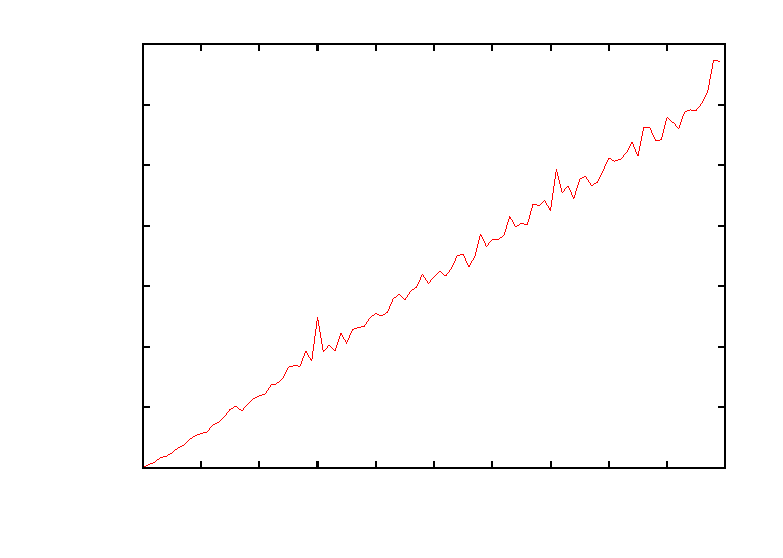
\includegraphics{n}}%
    \gplfronttext
  \end{picture}%
\endgroup

\caption{Experimentální ověření časové složitosti pro \(m = k = 4\).}
\label{fig:measurement_n}
\end{figure}

Cílem druhého experimentu bylo zjistit, jak se algoritmus chová při změnách rozměrů \(m\) a \(k\). Vstupem byly čtvercové matice se shodnými rozměry \(m = n = k\), pro každé měření se tedy měnil také počet potřebných procesorů. Při rozměru větším něž \(4\) již nebylo možné provést mapování procesu na jádro, tak jako v prvním experimentu. Pravděpodobně je to příčinou odchylek v měření zobrazeného grafem~\ref{fig:measurement_mk}, nicméně i přesto lze pozorovat exponenciální průběh. Exponenciální růst času byl očekáván, počet prvků vstupních čtvercových matic totiž roste s druhou mocninou jejich rozměru.
\begin{figure}
\centering
% GNUPLOT: LaTeX picture with Postscript
\begingroup
  \makeatletter
  \providecommand\color[2][]{%
    \GenericError{(gnuplot) \space\space\space\@spaces}{%
      Package color not loaded in conjunction with
      terminal option `colourtext'%
    }{See the gnuplot documentation for explanation.%
    }{Either use 'blacktext' in gnuplot or load the package
      color.sty in LaTeX.}%
    \renewcommand\color[2][]{}%
  }%
  \providecommand\includegraphics[2][]{%
    \GenericError{(gnuplot) \space\space\space\@spaces}{%
      Package graphicx or graphics not loaded%
    }{See the gnuplot documentation for explanation.%
    }{The gnuplot epslatex terminal needs graphicx.sty or graphics.sty.}%
    \renewcommand\includegraphics[2][]{}%
  }%
  \providecommand\rotatebox[2]{#2}%
  \@ifundefined{ifGPcolor}{%
    \newif\ifGPcolor
    \GPcolortrue
  }{}%
  \@ifundefined{ifGPblacktext}{%
    \newif\ifGPblacktext
    \GPblacktexttrue
  }{}%
  % define a \g@addto@macro without @ in the name:
  \let\gplgaddtomacro\g@addto@macro
  % define empty templates for all commands taking text:
  \gdef\gplbacktext{}%
  \gdef\gplfronttext{}%
  \makeatother
  \ifGPblacktext
    % no textcolor at all
    \def\colorrgb#1{}%
    \def\colorgray#1{}%
  \else
    % gray or color?
    \ifGPcolor
      \def\colorrgb#1{\color[rgb]{#1}}%
      \def\colorgray#1{\color[gray]{#1}}%
      \expandafter\def\csname LTw\endcsname{\color{white}}%
      \expandafter\def\csname LTb\endcsname{\color{black}}%
      \expandafter\def\csname LTa\endcsname{\color{black}}%
      \expandafter\def\csname LT0\endcsname{\color[rgb]{1,0,0}}%
      \expandafter\def\csname LT1\endcsname{\color[rgb]{0,1,0}}%
      \expandafter\def\csname LT2\endcsname{\color[rgb]{0,0,1}}%
      \expandafter\def\csname LT3\endcsname{\color[rgb]{1,0,1}}%
      \expandafter\def\csname LT4\endcsname{\color[rgb]{0,1,1}}%
      \expandafter\def\csname LT5\endcsname{\color[rgb]{1,1,0}}%
      \expandafter\def\csname LT6\endcsname{\color[rgb]{0,0,0}}%
      \expandafter\def\csname LT7\endcsname{\color[rgb]{1,0.3,0}}%
      \expandafter\def\csname LT8\endcsname{\color[rgb]{0.5,0.5,0.5}}%
    \else
      % gray
      \def\colorrgb#1{\color{black}}%
      \def\colorgray#1{\color[gray]{#1}}%
      \expandafter\def\csname LTw\endcsname{\color{white}}%
      \expandafter\def\csname LTb\endcsname{\color{black}}%
      \expandafter\def\csname LTa\endcsname{\color{black}}%
      \expandafter\def\csname LT0\endcsname{\color{black}}%
      \expandafter\def\csname LT1\endcsname{\color{black}}%
      \expandafter\def\csname LT2\endcsname{\color{black}}%
      \expandafter\def\csname LT3\endcsname{\color{black}}%
      \expandafter\def\csname LT4\endcsname{\color{black}}%
      \expandafter\def\csname LT5\endcsname{\color{black}}%
      \expandafter\def\csname LT6\endcsname{\color{black}}%
      \expandafter\def\csname LT7\endcsname{\color{black}}%
      \expandafter\def\csname LT8\endcsname{\color{black}}%
    \fi
  \fi
  \setlength{\unitlength}{0.0500bp}%
  \begin{picture}(7200.00,5040.00)%
    \gplgaddtomacro\gplbacktext{%
      \csname LTb\endcsname%
      \put(1078,704){\makebox(0,0)[r]{\strut{} 0}}%
      \put(1078,1383){\makebox(0,0)[r]{\strut{} 0.01}}%
      \put(1078,2061){\makebox(0,0)[r]{\strut{} 0.02}}%
      \put(1078,2740){\makebox(0,0)[r]{\strut{} 0.03}}%
      \put(1078,3418){\makebox(0,0)[r]{\strut{} 0.04}}%
      \put(1078,4097){\makebox(0,0)[r]{\strut{} 0.05}}%
      \put(1078,4775){\makebox(0,0)[r]{\strut{} 0.06}}%
      \put(1210,484){\makebox(0,0){\strut{} 0}}%
      \put(1831,484){\makebox(0,0){\strut{} 50}}%
      \put(2453,484){\makebox(0,0){\strut{} 100}}%
      \put(3074,484){\makebox(0,0){\strut{} 150}}%
      \put(3696,484){\makebox(0,0){\strut{} 200}}%
      \put(4317,484){\makebox(0,0){\strut{} 250}}%
      \put(4939,484){\makebox(0,0){\strut{} 300}}%
      \put(5560,484){\makebox(0,0){\strut{} 350}}%
      \put(6182,484){\makebox(0,0){\strut{} 400}}%
      \put(6803,484){\makebox(0,0){\strut{} 450}}%
      \put(176,2739){\rotatebox{-270}{\makebox(0,0){\strut{}Čas [s]}}}%
      \put(4006,154){\makebox(0,0){\strut{}Počet prvků matic}}%
    }%
    \gplgaddtomacro\gplfronttext{%
      \csname LTb\endcsname%
      \put(5816,4602){\makebox(0,0)[r]{\strut{}Naměřená data}}%
      \csname LTb\endcsname%
      \put(5816,4382){\makebox(0,0)[r]{\strut{}Bézierova křivka}}%
    }%
    \gplbacktext
    \put(0,0){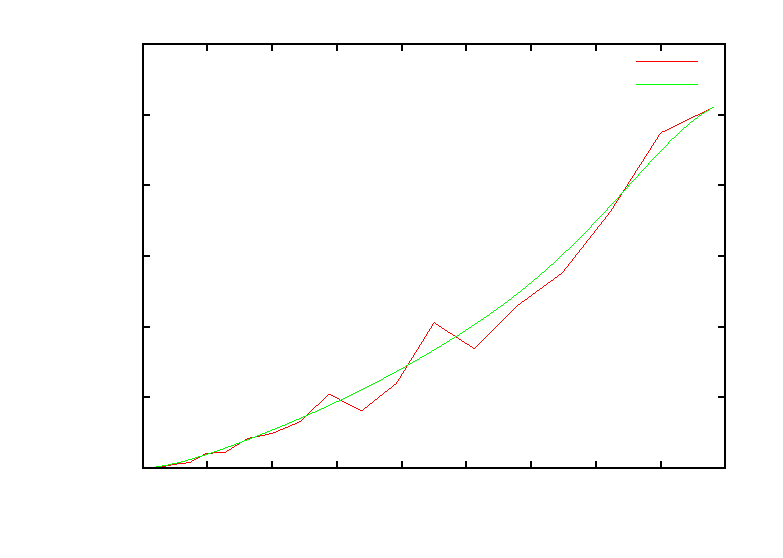
\includegraphics{mk}}%
    \gplfronttext
  \end{picture}%
\endgroup

\caption{Experimentální ověření časové složitosti.}
\label{fig:measurement_mk}
\end{figure}

%%%%
\section{Závěr}\label{conclusion}
%%%%
Rozbor v sekci~\ref{analysis} ukazuje, že teoretická časová složitost algoritmu mesh multiplication je lineární v závislosti na počtu prvků vstupních matic. Kvůli kvadraticky rostoucímu počtu procesorů ale algoritmus není optimální. Testy a experimenty uvedené v sekci~\ref{experiments} si kladly za cíl především ověřit teoretickou časovou složitost. Naměřené časy pro různé velikosti vstupních matic odpovídají lineárnímu průběhu a teoretickou složitos tak potvrzují také prakticky.

\end{document}
